% =====================================================================
% THE FACT OF FRACTAL TENNIS (TFOFT) — FINAL DRAFT
%  May 30 2026 With evertyhing so far
% =====================================================================

\documentclass[11pt,a4paper]{article}
\usepackage{amsmath}
\usepackage{amsfonts}
\usepackage{amssymb}
\usepackage{geometry}
\usepackage{booktabs}
\usepackage{longtable}
\usepackage{float}
\usepackage{mdframed}
\usepackage{hyperref}
\usepackage{verbatim}
\usepackage{graphicx}
\usepackage{tikz}
\usepackage{tabularx}
\usepackage{ragged2e}
\usepackage{array}
\setlength{\extrarowheight}{3pt}
\newcolumntype{C}[1]{>{\centering\arraybackslash}m{#1}}
\newcolumntype{L}[1]{>{\raggedright\arraybackslash}m{#1}}
\newcolumntype{Y}{>{\RaggedRight\arraybackslash}X}
\usetikzlibrary{calc, positioning, fit, backgrounds, arrows.meta, decorations.pathmorphing}
\graphicspath{{./figures/}}
\geometry{margin=1in}

\title{The Fact Of Fractal Tennis: \\
The Universe As A Fractal Computer Defined by the \\
Star=Electron+Atom=Galaxy Quine}
\author{Steven E.\ Elliott}
\date{May 2026}

\begin{document}

\maketitle
\begin{abstract}
  We propose a new principle of physics---MATHICCS---requiring that every mathematical axiom used in a physical law must correspond to an operation persistently realizable by a physical subsystem. Applying this criterion motivates reality's geometry as a discrete, self-similar, singularity-free structure: the Apollonian--Soddy Sphere Packing (ASSP). We conjecture that 3D dynamics on this packing is a self-computing fractal: a dynamical computer whose registers are fractal-congruent objects that process angular and linear momentum as cross-scale registers. This fractal quine is proposed as a self-consistent, MATHICCS-valid physical theory. It gives zero-free-parameter derivations of the baseline fine-structure constant \(\alpha^{-1}_{\rm TFOFT}=4\pi^3+\pi^2+\pi=137.036\), the electron--star logarithmic mass hierarchy, the electron mass, the proton mass, the proton/electron mass ratio, the 77-layer self-encoding register, the hydrogen binding energy, the hydrogen spectral ladder, and the gravitational constant \(G\) from atomic structure by two independent first-principles routes. We present empirical cross-checks involving the observed electron--star hierarchy, dark/visible channel fractions \(23/27\) and \(4/27\), Fermi-bubble morphology, the 25-arcminute CMB seam, and the near-match between Karlsson quasar logarithmic periodicity and the derived Info-channel leakage. The Karlsson complement also gives a 77-layer mass-channel spot check inside the same 137--139 register interval. We present one pending falsifiable prediction, \(\alpha^{-1}_{\rm Yb}=137.035998945\pm0.000000045\). The framework is presented as a zero-free-parameter ontology whose derived consequences are compared against major tensions in observational physics.
\end{abstract}

\begin{quote}
\textbf{Test criterion.}
A candidate fundamental law of the universe should be judged by three criteria. First, it should minimize free parameters: in golf-scoring fashion, every adjustable parameter is a penalty, because an unexplained parameter outsources part of the law to a non-provable external setter or to a deeper theory. A final law should therefore have zero, or at most one, free parameter. Second, it should derive or predict dimensionless constants rather than merely accept them as inputs. Third, it should satisfy the ordinary scientific standard of making quantitative predictions and surviving empirical tests.
\end{quote}

% ==================================================================
%  PART A:  MATHICCS => FRACTAL GEOMETRY
% ==================================================================


\section{Principles: The Motivation for MATHICCS}

\subsection{The Problem: Operational Constraints on Physical Axioms}

Modern physics often employs mathematical structures whose physical realization is left implicit. Consider:

\begin{enumerate}
  \item \textbf{Completed infinities} ($\mathbb{N}$ as a finished object): These are invoked in standard analysis and set theory but cannot be instantiated by any physical clock, apparatus, or experiment.
  \item \textbf{Limit operations at infinity} ($t \to \infty$, $V \to \infty$): No experiment can directly verify behavior at infinite time or volume.
  \item \textbf{Infinitesimal quantities and derivative-based formalisms}: Defined by $\epsilon$-$\delta$ limits that assume completion of infinite sequences.
  \item \textbf{Infinitely many degrees of freedom in field theory}: The continuum treats space as uncountably many points, exceeding what can be physically instantiated.
  \item \textbf{Black-hole singularities}: Divergent density and curvature indicate the model has left its domain of operational validity.
\end{enumerate}

These examples motivate a stricter criterion: a mathematical structure is physically admissible only if its defining operations can be realized by a persistent physical procedure.
\subsubsection{General Relativity and the DeSitter Collapse of Operational Clocks}

General relativity with $\Lambda > 0$ predicts that expanding FLRW solutions generically approach a de~Sitter-like late-time regime consistent with the observed cosmological constant~\cite{Planck2018VI}. In de~Sitter space the Gibbons--Hawking temperature~\cite{GibbonsHawking1977}
\[
T_{\rm dS} = \frac{\hbar c}{2\pi k_B} \sqrt{\frac{\Lambda}{3}}
\]
implies that finite-energy localized configurations are immersed in a horizon-temperature environment. A clock or apparatus of finite energy $E$ therefore has no eternal external reservoir from which to maintain, rebuild, or refine its operations. A characteristic decay scale may be written schematically as
\[
\tau_{\rm decay}(E) \sim \frac{3E}{\hbar c \Lambda}.
\]

This loss is not limited to freely expanding, unbound regions. Gravitationally bound systems do not provide permanent exceptions. In classical GR, generic nonstationary bound mass distributions carry time-dependent multipole structure and radiate gravitational waves. Unlike Newtonian gravity, GR does not give an eternally stable ideal two-body orbit: generic two-body motion has a time-dependent quadrupole moment, radiates gravitational waves, and inspirals. Bound gravitational motion is therefore a long-lived but finite reservoir of usable mechanical free energy, not a permanent foundation for an eternal limiting procedure.

The local inertial frame in GR also exhibits ordinary radiative physics. The Einstein Equivalence Principle asserts that, in a sufficiently small neighborhood of any event, nongravitational physics reduces to its special-relativistic form on the local Minkowski tangent frame. Thus the same local frame used to define clocks and rods also contains the usual Maxwell and Standard Model radiation channels: accelerated charges radiate by the Larmor channel; neutral but structured matter can radiate through time-dependent electric and magnetic multipoles; rotating magnetic configurations lose energy through magnetic dipole radiation; and weak processes can carry energy away through neutrinos.

\paragraph{The constructibility argument.}

The Einstein Equivalence Principle does not merely require that existing clocks keep ticking. It requires that \emph{at any spacetime point, in any state of motion}, one can \emph{construct} a local inertial frame by performing the limiting procedure of building ever-smaller apparatus. This is a \textbf{constructibility} claim, not a maintenance claim. The distinction matters.

For any finite energy $E > 0$, define $T_{\rm construct}(E)$ as the cosmic time after which it becomes impossible to construct---not merely maintain---a clock of energy $E$ at an arbitrary point in the expanding spacetime. Because the de~Sitter decay rate is nonzero, because bound mechanical stores are radiatively unstable in generic nonstationary configurations, and because the accessible comoving volume available for apparatus construction shrinks due to the cosmological horizon, $T_{\rm construct}(E)$ is finite for every $E > 0$:
\[
\exists\; T_{\rm construct}(E) < \infty \quad \forall\; E > 0.
\]
Hence no clock of energy $E$ can be constructed everywhere in the universe after cosmic time $T_{\rm construct}(E)$. The set of spacetime regions in which a valid $\varepsilon$-$\delta$ measurement apparatus can be \emph{constructed} therefore shrinks to measure zero:
\[
\mathcal{V}_{\rm constructible}(t) \to 0 \quad \text{as} \quad t \to \infty.
\]

\paragraph{Why the local limit does not rescue EEP.}

The usual defense of EEP is a spatial limiting argument. In a small freely falling laboratory of characteristic size $L$, curvature effects enter through tidal terms, schematically
\[
\epsilon_{\rm tidal}(L) \sim R L^2,
\]
so the metric becomes Minkowskian to arbitrarily good accuracy as $L\to0$. This is the standard reason one says curvature can be transformed away at a point.

MATHICCS asks a different question: can the limiting procedure itself be physically constructed and repeated inside the universe described by the same theory? The limit $L\to0$ is not a magic symbol. It is a sequence of apparatus constructions, synchronizations, refinements, and readouts. In a universe with $\Lambda>0$, the accessible region and usable free energy available for such constructions decay with cosmic time. Thus the physical support of the EEP limit is time-dependent.

The conflict is between two scalings. Spatially, the local inertial approximation improves quadratically:
\[
\epsilon_{\rm tidal}(L)\sim R L^2.
\]
Temporally, the set of regions in which the required apparatus can be constructed shrinks under de~Sitter horizon dynamics:
\[
\mathcal{V}_{\rm constructible}(t)\sim \mathcal{V}_0 e^{-\gamma t},
\]
for some positive effective decay rate $\gamma$. The exact coefficient is not important here; the important point is that the constructible domain decreases monotonically to zero while the EEP limit requires an indefinitely repeatable physical construction.

Thus EEP wins only as a formal spatial limit at fixed time. It does not win as a persistent physical axiom over the full future history of a $\Lambda>0$ universe. As $t\to\infty$,
\[
\mathcal{V}_{\rm constructible}(t)\to0,
\]
so the limiting procedure required to realize $L\to0$ has no positive-measure domain left on which to operate. In this sense, EEP holds nowhere in the MATHICCS sense at future infinity: not because the formal tangent space cannot be written down, but because the physical procedure that gives the tangent space operational meaning can no longer be instantiated.

The long lifetime of macroscopic clocks does not change this conclusion. A large $\tau_{\rm decay}$ only delays the collapse of the constructible domain. It does not convert a finite-duration construction into a persistent axiom. Foundational axioms cannot depend on an expiring supply of physical realizers.

This can be stated as a clean theorem-like result:

\begin{quote}
\textbf{Theorem-like statement.} In any spacetime with $\Lambda>0$, the standard EEP argument gives a local spatial limit, not a persistent physical realizer. Curvature errors inside a laboratory of size $L$ fall as $O(L^2)$, but the positive-measure domain in which the required sequence of ever-smaller laboratories can be constructed decays to zero over cosmic time. Therefore, for every finite apparatus energy $E>0$, there exists a finite cosmic time $T_{\rm construct}(E)$ after which the constructive limiting procedure required by EEP cannot be carried out at an arbitrary spacetime point. Gravitational binding can delay this failure but cannot eliminate it, because generic bound systems radiate and realistic local matter fields leak energy through electromagnetic and weak channels. EEP is therefore not a MATHICCS-valid foundational axiom: it is an approximation with a finite domain of constructive validity. General relativity with $\Lambda>0$ is operationally self-limiting under MATHICCS.
\end{quote}

\subsubsection{The Role of External Formalism}

Independence results in set theory, Gödel incompleteness, and non-constructive continuum assumptions indicate that not every mathematically coherent object is automatically physically realizable~\cite{Godel1931}.

MATHICCS does not invalidate calculus as a computational tool. It distinguishes ontological claims (the continuum \emph{is} reality) from effective approximations (the continuum \emph{describes} reality to bounded error). A computable calculus grounded in ASSP sphere geometry is fully MATHICCS-valid.

\subsection{MATHICCS: The Operational Criterion}

We propose the following criterion.

\begin{quote}
A mathematical axiom is physically valid if and only if there exists a physical subsystem that can instantiate the operation described by the axiom and do so persistently under the evolution laws of the system partially or wholly described by that same axiom.
\end{quote}

This criterion is called MATHICCS: \emph{Mathematical Axioms That Have Infinitely Complete Computable Sanity}.

\subsubsection{Definition 1: Mathematical Process $P$}
A mathematical process $P$ is any logical operation that appears in an axiom (quantifier, limit, smoothness assumption, cardinality statement, integral, etc.).

\subsubsection{Definition 2: Internal Realizer}
An internal realizer is a subsystem $S$ composed of clocks, apparatus, and protocols that can instantiate process $P$ to arbitrary finite precision, with precision arbitrarily improvable by expanding $S$.

\subsubsection{Definition 3: Internal Persistence}
Process $P$ has internal persistence if there exists a positive-measure set of initial states under which the creation of realizers of $P$ survives indefinitely under the evolution laws dictated by the axioms containing $P$.

\subsubsection{Definition 4: MATHICCS Axiom M1 --- Operational Validity}
An axiom $A$ containing process $P$ is MATHICCS-valid only if $P$ has internal persistence. This is the Elliott Math Stability Rule (EMSR).

\subsubsection{Definition 5: MATHICCS Axiom M2 --- Internal Realization}
Physical meaning requires demonstration of internal realization. Axioms drawn purely from external set theory, Peano arithmetic, ZFC, large cardinals, or completed $\epsilon$-$\delta$ limit processes are not physically admissible unless grounded in a physical subsystem. This is the Internal Realization Requirement (IRR).

\subsubsection{Definition 6: MATHICCS Axiom M3 --- Ontological Self-Consistency}
An ontology $O$ is valid only if all axioms in $O$ satisfy M1 and M2 simultaneously. An ontology that is MATHICCS-valid and matches universal observations to bounded error satisfies the ontological-epistemological equivalence principle (OEEP).

\subsection{Why Self-Describing Systems Must Be G\"odel-Free}

A self-describing physical system is one in which the laws governing the system are themselves encoded as structures within the system. This is the setting in which MATHICCS applies: the realizers of the axioms must persist under the laws those axioms describe.

\begin{quote}
\textbf{Theorem (Informal):} A MATHICCS-valid self-describing system cannot be governed by an axiomatic system subject to G\"odel incompleteness.
\end{quote}

\textit{Argument.} Suppose the system $\mathcal{U}$ is described by an axiomatic system $\mathcal{A}$ that is G\"odel-incomplete. Then there exists a true statement $S$ about $\mathcal{U}$'s dynamics that $\mathcal{A}$ cannot prove. But $\mathcal{U}$ must physically realize its own dynamics, including the dynamics described by $S$. This means that $\mathcal{U}$ performs an operation that its own descriptive language cannot validate. Under M1 any operation in $\mathcal{U}$ must be persistently realizable. A MATHICCS-valid self-describing system is therefore naturally modeled by a complete, consistent, decidable axiomatic framework.

Among known arithmetic systems, Presburger arithmetic (addition and order only, without general multiplication) is complete, consistent, and decidable~\cite{Presburger1929}. These properties make it a natural candidate for the internal arithmetic of a self-describing physical theory.


\section{Fractal Law: From MATHICCS to Fractal Geometry}

\subsection{Why MATHICCS Motivates a Fractal Substrate}

\subsubsection{Step 1: Replace the Continuum}
Standard physics uses $\mathbb{R}$ as the arena for continuous fields, while fractal geometry provides a well-developed language for scale-recursive structures in nature~\cite{Mandelbrot1983,Nottale2011}. However, $\mathbb{R}$ is a completed infinity: it contains uncountably many points with no constructive specification. Under M2 this is not an automatically admissible physical assumption. A possible alternative is a recursively refinable discrete structure. At level $n$ there are $N_n$ discrete positions; at level $n+1$ there are $N_{n+1}=kN_n$ for some $k>1$. This replaces completed infinity with unbounded recursion.

\subsubsection{Step 2: Require Persistent Structure}
For a physical subsystem to persist, its construction must be stable under evolution. Continuous fields can develop singularities, while discrete self-similar structures avoid such singular points at every scale. This makes self-similar discrete geometry an attractive candidate for a MATHICCS-valid substrate.

\subsubsection{Step 3: Fractal Conclusion}
Taken together, these considerations suggest that a universe governed by MATHICCS should be discrete at finite resolution, self-similar across scales, stable under its own dynamics, and determined by local tangency relations. The appropriate coarse description of reality is therefore an unbounded fractal with no preferred smallest or largest scale.

\subsubsection{Step 4: Empirical Selection by Dual Monofractal Scaling}
The ASSP is selected by combining the MATHICCS requirement with the observed dual monofractal pattern in dynamical systems. The 3D bulk channel repeatedly exhibits Soddy-like scaling near \(D_S\approx2.47\), while 2D boundary layers, radial cuts, rotational interfaces, and shell-like transport channels repeatedly exhibit Apollonian-like scaling near \(D_A\approx1.305\). A substrate built from recursive tangent spheres naturally contains both channels in the same object: the 3D packing supplies the bulk Soddy family, and the boundary/interface cuts supply the Apollonian family. Thus the ASSP is proposed as the minimal MATHICCS-valid candidate because it gives one recursive mechanism for the two observed exponent families of the same dynamic system.

% ==================================================================
%  PART B:  EMPIRICAL EVIDENCE FOR THE FRACTAL ASSP
% ==================================================================


\section{Evidence for the Fractal ASSP}

The principal motivation for the present proposal is the persistence of approximately flat galactic rotation curves, as observed in spiral galaxies including the Milky Way and Andromeda~\cite{Sofue2012,Chemin2009}, which indicates that orbital speeds remain near-constant over a substantial radial range rather than declining in the Keplerian manner expected from the visible baryonic distribution alone. At the atomic scale, a closely related regularity appears in the quantization of emission frequencies: photons are emitted only at discrete transition frequencies, with photon energy proportional to frequency through $E_{\rm photon}=h\nu$.

Within the present hypothesis, these two phenomena are treated as scale-related manifestations of a common transfer mechanism. The atom provides the lower-scale electron-to-photon channel, while the galaxy core is conjectured to play the corresponding role for a star-to-macrophoton channel. The observed flat rotation curve would then arise as the lower-scale projection of a quantized energy-transfer law operating at the higher fractal level.

The empirical case for fractal congruence between atomic and galactic scales---including a $\sim31\%$ viscous drag signature consistent with a scaled electron-shell contribution to stellar orbital dynamics---is developed in detail in the companion paper \cite{FSEquivalence2026}. The present paper takes these findings as established and proceeds to the geometric derivation.

\subsection{Power Laws and the Apollonian-Soddy Fractal Dimension}

\subsubsection{Why The ASSP?}

A self-similar discrete packing is a natural candidate for a three-dimensional geometry that is simultaneously dense, recursive, and free of singular points, in the spirit of classical fractal geometry and Apollonian packing theory~\cite{Mandelbrot1983,Boyd1973,Graham2003,Manna1991}. Sphere packings admit recursive nesting, avoid edge singularities, and can be specified locally through tangency relations. Among such packings, the Apollonian--Soddy sphere packing is distinguished by its exact recursive geometry and by the determinacy of the Descartes--Soddy curvature relation~\cite{Soddy1936,Boyd1973,Graham2003}.

The empirical selection criterion is the dual monofractal power-law pattern. The same dynamic substrate must generate both the Soddy-like 3D bulk exponent family and the Apollonian-like 2D boundary/interface exponent family. The ASSP has this structure internally: the full sphere packing supplies recursive 3D bulk scaling, while tangent boundaries, radial cuts, and rotational interfaces supply the corresponding 2D Apollonian projections. The proposed substrate is therefore selected by the combination of finite recursive realizability and observed dual-channel monofractal scaling.

More precisely:
\begin{itemize}
  \item \textbf{Perfect self-similarity}: the packing in any region is identical to the packing at any scale, up to constant rescaling.
  \item \textbf{Determinate geometry}: given mutually tangent spheres, the Soddy curvature relation determines subsequent configurations uniquely up to reflection.
  \item \textbf{Dual-channel scaling}: the same recursive object contains a 3D Soddy bulk channel and 2D Apollonian boundary/interface channels.
\end{itemize}

\subsubsection{Observed Fractal Dimensions}

Across a wide range of systems in physics, biology, economics, and geophysics, power-law exponents frequently cluster near values associated here with Apollonian and Soddy-type recursive geometries~\cite{Mandelbrot1983,Manna1991,Boyd1973}:
\begin{itemize}
  \item $\alpha\approx1.3$: Apollonian gasket dimension ($D_A=1.305$)
  \item $\alpha\approx2.4$: Soddy sphere packing dimension ($D_S=2.47$)
\end{itemize}
The important fact is not merely that power laws occur. Many mechanisms can generate approximate power laws over a narrow regime. The stronger fact is that similar exponent families recur across many apparently unrelated systems and across widely separated physical scales. Persistent scale-independent power-law behavior is the natural signature of a recursive generator. If the same scaling families appear at all observed scales, then the simplest explanation is not a collection of unrelated local mechanisms, each accidentally producing the same exponents, but a common fractal substrate.

In ordinary critical phenomena, power laws usually appear near a special transition, with finite correlation length, finite scaling window, and system-specific universality class. A truly scale-independent recurrence across astrophysical, geophysical, biological, chemical, and informational systems points to a different kind of explanation: a monofractal generator, or a tightly coupled dual projection of one generator. In the present proposal the generator is not two unrelated fractals. It is the same Apollonian--Soddy recursive packing seen in two ways: the 3D bulk packing gives Soddy-like exponents near $D_S\approx2.47$, while 2D boundary layers, radial cuts, and rotational interfaces give Apollonian-like exponents near $D_A\approx1.305$.

This is why the distinction between the two exponent families matters. Power-law exponents near $D_A \approx 1.3$ recur specifically in systems with radially defined, boundary-dominated, or rotationally dominated dynamics, such as river networks, coastlines, galactic two-point correlation functions, and shell-like transport structures. Exponents near $D_S\approx2.4$ recur in bulk filling, branching, packing, or filamentary systems, such as cosmic web density, interstellar structure, stellar mass functions, lung branching, and QCD-like flux tubes. Under TFOFT these are not independent coincidences. They are the 2D boundary and 3D bulk expressions of the same ASSP generator.

\subsubsection{Universal Power-Law Table}

\begin{longtable}{p{6.8cm}ccc}
\caption{Representative power laws across multiple domains, grouped by their proximity to Apollonian or Soddy scaling.} \\
\toprule
\textbf{System} & \textbf{Exponent} & \textbf{Fractal $D$} & \textbf{Type} \\
\midrule
\endfirsthead
\toprule
\textbf{System} & \textbf{Exponent} & \textbf{Fractal $D$} & \textbf{Type} \\
\midrule
\endhead
\midrule\multicolumn{4}{r}{\textit{Continued on next page}}\\\endfoot
\bottomrule\endlastfoot

\multicolumn{4}{l}{\textit{Astrophysical and Cosmological}} \\
\midrule
Galaxy two-point correlation function & $1.77$ & $\approx1.2$ & Apollonian \\
Cosmic web filament density profile & $\approx2.4$ & $\approx2.4$ & Soddy \\
Interstellar medium density fluctuations & $\approx2.4$ & $\approx2.4$ & Soddy \\
Dark matter halo mass function & $1.8$--$2.0$ & $\approx2.4$ & Apollonian/Soddy \\
Stellar mass function / IMF (Salpeter) & $2.35$ & $\approx2.4$ & Soddy \\
Solar wind turbulence spectrum & $5/3\approx1.67$ & $\approx1.2$ & Apollonian \\
Cosmic ray energy spectrum & $\approx2.7$ & $\approx2.4$ & Soddy \\
Asteroid size distribution & $\approx2.5$ & $\approx2.4$ & Soddy \\

\midrule
\multicolumn{4}{l}{\textit{Geophysical and Environmental}} \\
\midrule
Earthquake energy (Gutenberg--Richter) & $1.8$--$2.2$ & $\approx2.4$ & Apollonian/Soddy \\
Forest fire size distribution & $1.3$--$1.9$ & $\approx1.2$ & Apollonian \\
River network branching (Horton's law) & $\approx1.2$ & $\approx1.2$ & Apollonian \\
Coastline fractal dimension (global avg) & $\approx1.2$ & $\approx1.2$ & Apollonian \\

\midrule
\multicolumn{4}{l}{\textit{Physical and Chemical}} \\
\midrule
Turbulent energy spectrum (Kolmogorov) & $\approx1.67$ & $\approx1.2$ & Apollonian/Soddy \\
Crack propagation / fracture events & $1.2$--$2.0$ & $\approx1.2$ & Apollonian \\
Magnetic Barkhausen noise & $1.3$--$1.8$ & $\approx1.2$ & Apollonian \\
QCD flux tube (strong force) & $\approx2.4$ & $\approx2.4$ & Soddy \\

\midrule
\multicolumn{4}{l}{\textit{Biological}} \\
\midrule
Neuronal avalanche sizes in cortex & $\approx1.5$ & $\approx1.2$ & Apollonian \\
Neural dendritic arbor dimension & $1.2$--$1.4$ & $\approx1.2$ & Apollonian \\
Lung bronchial branching & $\approx2.4$ & $\approx2.4$ & Soddy \\
Gene regulatory network connectivity & $2$--$3$ & $\approx2.4$ & Soddy \\

\midrule
\multicolumn{4}{l}{\textit{Human, Social, and Informational}} \\
\midrule
Word frequency distributions (Zipf) & $1$--$2$ & $\approx1.2$ & Apollonian \\
City size distributions (Zipf) & $1$--$2$ & $\approx1.2$ & Apollonian \\
Wealth distribution (Pareto tail) & $1.5$--$3$ & $\approx2.4$ & Apollonian/Soddy \\
Internet topology & $2$--$3$ & $\approx2.4$ & Soddy \\
\end{longtable}

\subsubsection{Conclusion: The Fractal Dimension Argument}

The recurrence of exponents near the Apollonian and Soddy values is not, by itself, sufficient to prove a unique underlying mechanism. However, identical or near-identical power-law families across many observed scales require explanation. Local mechanisms can produce local power laws; they do not naturally explain why the same exponent families keep reappearing in unrelated domains. A common recursive generator does.

The ASSP supplies such a generator with one ontology rather than many fitted mechanisms. Its 3D bulk recursion produces Soddy-like scaling, while its 2D boundary cuts and radial interfaces produce Apollonian-like scaling. The observed pattern is therefore consistent with a single fractal law appearing as a dual projection: bulk versus boundary, 3D packing versus 2D interface. This is the empirical basis for the conjecture stated in Section~\ref{sec:conjecture}.


\begin{figure}[htbp]
\centering
\includegraphics[width=0.95\textwidth]{./figures/tfoft_figure_assp_level_7.png}
\caption[Soddy Sphere Packing Iteration 7]
{Opaque outline of the tetrahedral seed generating the Soddy cores inside the virtual outer Soddy sphere.}
\label{fig:soddy_layer_7}
\vspace{1.2em}
\textbf{Credit:} Generated by Steven E. Elliott.
\end{figure}

% ==================================================================
%  PART C:  PRIOR FRACTAL PHYSICS AND THE QUINE GAP
% ==================================================================


\section{Prior Fractal Physics and the Closure Problem}
\label{sec:conjecture}

\subsection{A Survey of Fractal Physics Attempts}

Fractal geometry has attracted serious attention in physics for decades. Each approach captured part of the truth, but none reached the full self-computing picture. A brief survey:

\begin{itemize}
  \item \textbf{Mandelbrot (1977--1983):} Established that natural systems exhibit fractal geometry; identified power-law scaling and self-similarity as universal features, but offered no dynamical mechanism~\cite{Mandelbrot1983}.
  \item \textbf{Garnet Ord / Chaos theory QM (1983):} Showed that random walks on fractal lattices recover structures analogous to relativistic quantum mechanics; insightful but external rules imposed, not self-generated~\cite{Ord1983}. This result provides important mathematical support for the TFOFT framework.
  \item \textbf{Halton Arp's intrinsic redshift / fractal cosmology (1987--):} Observed that quasar redshift clusters at preferred values and argued against the Big Bang space expansion metric; the logarithmic periodicity is historically associated with Karlsson's preferred-redshift relation~\cite{Karlsson1971,Mal2020}, but no mechanism for the discretization was provided.
  \item \textbf{Nottale's Scale Relativity (1992--):} Extended relativity to non-differentiable, fractal spacetime and derived quantum-like behavior from fractal geodesics~\cite{Nottale2011}; formally elegant but still grounded in the continuum and limit operations, violating M1. The theory identified the physical law as fractal but did not define congruent physically fractal objects, leaving M3 unaddressed.
  \item \textbf{El Naschie's E-infinity theory (1990s--2000s):} Proposed that spacetime has a fractal Cantorian microstructure with dimension related to the golden ratio; derived $\alpha^{-1}\approx137$ from Cantorian set theory~\cite{ElNaschie1997}, but relied on completed infinities and non-constructive objects, violating MATHICCS M2.
  \item \textbf{Lestone's string-surface model and $\alpha$ (2007):} Proposed that the fine-structure constant emerges from a heuristic string-like particle-surface model constrained by assumptions inspired by Apollonian circle packing geometry~\cite{Lestone2007}. This yields $\alpha \approx 1/137.04$ without peer review or independent confirmation. It remains the closest geometric precursor to the ASSP but lacks any computational architecture, self-referential quine mechanism, or explicit fractal congruent objects.
\end{itemize}

\subsection{Ord's Fractal Space-Time and the Star-Electron Congruence}

Ord (1983) starts from the observation that quantum particle paths are highly irregular and non-differentiable when examined at fine enough scales, and constructs a fractal spacetime analogue of relativistic quantum mechanics~\cite{Ord1983}. He constructs a continuous but fractal trajectory in spacetime (exemplified by a space-filling Peano-Moore curve with Hausdorff dimension exactly 2 instead of the classical dimension 1). The particle is confined to move on these fractal paths in both space and time. This geometric setup naturally reproduces key quantum features: the uncertainty principle, the de Broglie relation, interference effects, and aspects of relativistic quantum mechanics --- all without invoking the full machinery of the Schrödinger equation or path integrals from the start.

When we treat stars as fractal-scale congruents of electrons, and consider electron dynamics to be the low-to-high velocities of ballistic stellar dynamics, which would act like random walks on fractal lattices due to the fractal-like large-scale observed cosmic web structure, this provides direct mathematical support for the cross-scale congruence between stars and electrons in TFOFT.

\subsection{The Closure Problem: The Fractal Quine}

The theories surveyed above establish important parts of the fractal-physics program. The remaining closure problem is self-reference: the fractal law must be encoded, transmitted, and enforced by objects inside the same fractal system.

A complete fractal ontology must answer the deeper question: \textbf{where do the rules come from, and how does the system enforce them on itself?}

The answer requires three ingredients:

\begin{enumerate}
  \item \textbf{A MATHICCS-valid axiomatic foundation} (Presburger arithmetic~\cite{Presburger1929}) that is complete, consistent, and decidable---so the system can describe its own operations without Gödel breakage or non-provable, non-physical, non-testable, external processes.

  \item \textbf{A self-computing architecture.} The dynamical ASSP is conjectured to be not merely a geometric pattern but a dynamical computer. Fractal congruent objects in a fluid-like dynamical system can chaotically evolve into a self-annealing (AI-like) computer system analogous to Turing machines~\cite{VonNeumann1966,Wolfram2002}; those fractal congruent objects would then constitute the dynamical computational basis.

  \item \textbf{The photonic mechanism.} The later FTC ontology identifies a cross-scale transport channel in which angular momentum is carried by Info Balls, while the computational cost of the transfer is paid into lower-scale linear momentum as Dust Ball production. This converts the fractal from a static pattern into a self-running program: the rules are not merely imposed on the packing, but transmitted and paid for by the packing's own dynamics.
\end{enumerate}

\begin{quote}
\textbf{A fractal that follows external rules is a pattern. A fractal whose rules are encoded, transmitted, and enforced by its own dynamics is a quine. TFOFT is the first attempt at a MATHICCS-valid fractal quine theory of physics.}
\end{quote}

% ==================================================================
%  PART D:  ONTOLOGY --- THE FRACTAL TENNIS COMPUTER
% ==================================================================

\section{The Presburger--ASSP Register Basis and Derived Constants}
\label{sec:ftc}


\subsection*{Status of Claims}

This paper combines established mathematical structure with new physical
identifications and conjectures. The categories used throughout are:

\begin{itemize}
  \item \textbf{Established background:} standard mathematical and physical
  results such as Presburger decidability, the Descartes--Soddy relation,
  Apollonian packing structure, and measured observational quantities.

  \item \textbf{Definitions:} terminology introduced by the present paper,
  including Star Ball, Core Ball, Gyro Ball, Info Ball, Dust Ball, and the
  Presburger--ASSP machine, named the Fractal Tennis Computer (FTC) at the
  start of the machine section below.

  \item \textbf{Conjectures:} proposed identifications between the ASSP
  structure and observed systems, including star/electron congruence,
  atom/galaxy congruence, dark matter as lower-scale substrate, and force
  channels as tangency orders.

  \item \textbf{Derived quantities:} quantities obtained internally from the
  ontology and cost model, including
  \(T_{\rm sphere}=4\pi^3+\pi^2+\pi\),
  \(\alpha^{-1}_{\rm TFOFT}=T_{\rm sphere}\),
  the rank-23 channel split,
  the half-boundary mass register,
  and the resulting 77-layer closure.
\end{itemize}

Notation distinguishes internally derived quantities
(\({\rm TFOFT}\)) from observed astrophysical/cosmological quantities
(\({\rm obs}\)) and laboratory measurements (\({\rm meas}\)).

Thus \(k_{\rm mass}^{\rm TFOFT}\),
\(T_{\rm mass}^{\rm TFOFT}\), and
\(S_{\rm mass}^{\rm TFOFT}\) are ontology-internal quantities, while
\(\ln(M_\odot/m_e)_{\rm obs}\),
\(G_{\rm meas}\), and
\(\alpha_{\rm meas}\) are observational or laboratory comparison values.


\subsection{The Fractal Tennis Computer (FTC)}

The Presburger--ASSP computational machine is hereafter called the \textbf{Fractal Tennis Computer} (FTC). The FTC is the self-computing ASSP register system whose active objects are Star Balls, Core Balls, Gyro Balls, Info Balls, Dust Balls, and their boundary channels. The name emphasizes the dynamical picture: angular-momentum information is served, received, reflected, and reconstructed across tangent spherical registers, while the computational cost of each transfer is paid into lower-scale linear-momentum substrate.

Standard mathematical formulations of the Standard Model and General Relativity are normally expressed using continuum analysis and arithmetic strong enough to fall within the scope of Gödel-style incompleteness results~\cite{Godel1931}. These systems cannot prove all true statements about their own arithmetic, creating a fundamental barrier to self-description. In contrast, Presburger arithmetic (addition and order only, without general multiplication) is complete, consistent, and decidable~\cite{Presburger1929}. Multiplication by a \emph{constant} is implemented via repeated addition and is therefore valid; only variable-by-variable multiplication requires indirection. As established in Section~1.3, a MATHICCS-valid self-describing universe is naturally modeled by this arithmetic.

The dynamical Apollonian-Soddy sphere packing (ASSP) operating under Presburger arithmetic is conjectured to constitute a universal computational machine. Unlike the idealized infinite-tape Turing machine, the ASSP machine operates on \emph{finite but recursively expandable tape}, closer in spirit to finite physical computation and self-reproducing automata~\cite{VonNeumann1966,Fredkin1990,Wolfram2002}. At each fractal layer $N$, the accessible substrate is a locally finite sphere packing with a bounded number of active tangencies. When those tangencies are exhausted, the machine descends to layer $N-1$, adding a finite increment of new capacity. Each expansion step is governed by the Soddy curvature relation, which is a decidable, closed-form computation.

\subsubsection{Why the FTC Is G\"odel-Free}
\label{sec:godel_free}

G\"odel incompleteness applies to sufficiently expressive formal systems that internalize arithmetic over completed infinite domains and support the fixed-point machinery needed for diagonal self-reference~\cite{Godel1931}. The FTC is constructed to avoid precisely that internalization. Its arithmetic core is Presburger arithmetic: addition, order, finite indexing, and finite combinatorial structure, without primitive variable-by-variable multiplication as a completed total operation~\cite{Presburger1929}.

The important point is not that the machine has an indefinitely extendable tape in the Turing-machine sense. It does not contain an actually completed unbounded tape as an internal object. At every stage the active substrate is a finite Soddy tangency configuration with finite addresses, finite local neighborhoods, finite proof chains, and finite computation traces. Further refinement is allowed only as a new finite trace step governed by the Soddy curvature relation. The limit of endless refinement is a boundary idealization, not an internal domain of quantification.

Thus the FTC uses potential infinity rather than completed infinity. One may always perform another finite refinement, descend one more fractal layer, or extend a finite address by one more symbol. But the completed infinite branch, the completed graph of multiplication, the completed set of all traces, and the completed self-referential fixed point are not admitted as internal objects. Finite cells and finite traces are internal, while the limiting Cantor-dust boundary of possible completions remains external and non-internal.

The fractal quine derived in Section~\ref{sec:quine} requires approximately 77 recursive log-steps (derived in Section~\ref{sec:mass_channel}) to complete one self-encoding cycle. These 77 steps are not an appeal to an infinite tape. The machine reads and writes a finite number of Soddy tangency states, executes a finite number of Presburger-valid additions and comparisons, and terminates in a new finite configuration at the next scale layer. After the cycle, the machine has reproduced the relevant register pattern, but it has not quantified over an infinite set or completed a total recursive universe.

\begin{quote}
\textbf{Axiom P3 (Finite Trace Extension):} A MATHICCS-valid self-describing machine executes only finite trace steps over finite Soddy tangency configurations. Each refinement step must have a finite address, a finite local rule, and a decidable Presburger description. Recursive extension is potential: the system may always generate a further finite trace, but it never internalizes the completed infinity of all traces, all branches, or all self-referential fixed points. The FTC satisfies this through local fractal refinement governed by the Soddy curvature relation. G\"odel incompleteness does not obstruct this physical execution because the machine never performs unbounded quantification over a completed infinite domain and never admits the completed diagonal object as an internal state.
\end{quote}

This distinction explains why QFT and GR are not MATHICCS-valid in the sense of M2: both employ completed real-number continua and mathematical induction over completed infinite domains. The FTC does not deny approximation, convergence, recursion, or analysis. It rejects the promotion of arbitrary nonconstructive limits into internal physical objects. Its computations are finite traces on finite tangency states, with further refinement always possible but never completed.


\subsection{Basis Radius Selection: Physical Word Size and Presburger Cost Minimization}
 
Presburger arithmetic lacks general variable multiplication; all operations reduce to repeated addition and finite symbol manipulation. In the FTC, every symbol, operation, and lookup constitutes a physical computational cost.

\paragraph{Numbers as programs; the word-size question.}

A critical clarification is required before the cost model can be stated. MATHICCS contains no abstract numbers. Every quantity in the FTC is a \emph{physical program or circuit} executed by the substrate of no-slip rotating spheres in a sphere packing. The symbol ``$\pi$'' is not a transcendental real number imported from external mathematics; it is the program that a sphere executes when it reports its own circumference-to-diameter ratio---a directly and persistently realizable physical operation on the substrate.

The analogy to digital computing is precise. On a digital circuit, \texttt{u32(1)} and \texttt{u8(1)} are not the same object even though both represent the concept of ``one.'' The word size is determined by the physical register, not by abstract arithmetic. Asking whether $\pi$ is ``allowed'' in Presburger arithmetic commits the same error as asking whether a 32-bit register is ``allowed'' to hold a value that doesn't fit in 8 bits: it confuses the arithmetic with the hardware. 
In the FTC, the physical registers are literal spheres undergoing no-slip rotation in a sphere packing. The natural \emph{word size} of this substrate---the primitive quantity that every physical operation either reads or writes---is the sphere itself. The sphere's intrinsic dimensional unit is its radius, and it's intrinsic non-dimensional unit is the constant ratio of its circumference to its diameter---$\pi$. This is not chosen; it is measured from the register.

The basis-radius selection problem is therefore not ``which transcendental number should we allow in our integer arithmetic?'' It is:

\begin{quote}
\textbf{Which sphere radius, expressed as a multiple of the substrate's own natural unit, minimizes the total Presburger execution cost of the fractal quine's state-update program?}
\end{quote}

Presburger arithmetic governs the \emph{operations}---addition and order only, with multiplication by a constant implemented as repeated addition. The \emph{basis symbol} is determined by the physical substrate and is not subject to Presburger's domain restriction. Presburger minimization then selects among configurations expressible as repeated additions of that basis symbol---which is precisely what Presburger arithmetic permits.

\paragraph{Cost model.}

The relevant cost is the total execution cost of the state-update program:
\[
C(\mathcal{P}) = C_{\rm lookup} + C_{\rm op} + C_{\rm reuse},
\]
where:
\begin{itemize}
  \item $C_{\rm lookup}$ counts distinct symbol retrievals,
  \item $C_{\rm op}$ counts repeated-addition execution cost,
  \item $C_{\rm reuse}$ rewards reuse of already-instantiated basis symbols
    across multiple channels.
\end{itemize}

The complete state-update cost for a single Soddy sphere contains three independent channels:
\[
T_{\rm sphere}(r) = 4\pi r^2 + \pi r + r.
\]

The optimization problem is:

\begin{quote}
Choose the basis radius $r$---expressed as a Presburger-valid multiple of the substrate's natural unit---minimizing total fractal-quine execution cost by maximizing symbol reuse and minimizing distinct lookup operations during recursive state updates.
\end{quote}

Two representative choices illustrate the result:

\begin{itemize}
  \item \textbf{Choice $r = 4$ (four sphere-radii as basis):}
  \[
  T_{\rm sphere}(4) = 64\pi + 4\pi + 4 \approx 217.6.
  \]
  The program must maintain two distinct persistent symbols---the geometric constant $\pi$ (the substrate's natural unit) and the separate basis radius $4$. These are two different programs the machine must instantiate and keep available across every recursive update. Symbol reuse is partial.

  \item \textbf{Choice $r = \pi$ (one sphere-radius as basis):}
  \[
  T_{\rm sphere}(\pi) = 4\pi^3 + \pi^2 + \pi \approx 137.036.
  \]
  Here the basis radius and the substrate's natural geometric unit are the
  \emph{same persistent symbol}. Every channel in the state-update program
  reads from the single physical program that a sphere executes to report its
  own geometry. One distinct symbol class is eliminated from the recursive
  lookup table entirely.
\end{itemize}

The reduction is not merely numerical but computational. When $r = \pi$, the fractal quine executes fewer recursive symbol-resolution steps because the sphere radius, rotational arc-length scale, and geometric curvature constant collapse into a single reusable substrate program. This is the \emph{physical} content of the minimization: not that $\pi$ is a pretty number, but that a sphere packing whose registers are spheres has only one natural word size, and the minimum-cost program uses that word size as its basis rather than introducing a second incommensurable symbol.

\begin{quote}
\textbf{Axiom P2 (Presburger Minimization Principle):}
A MATHICCS-valid self-describing machine selects the basis radius minimizing total recursive execution cost under Presburger operations. For a substrate of no-slip rotating spheres in a sphere packing, the substrate's own natural unit is $\pi$---the ratio of circumference to diameter, directly and persistently realizable as a physical operation on the register. The unique basis radius satisfying maximal geometric-symbol reuse across all three independent Soddy state channels is therefore:
\[
\boxed{r = \pi}.
\]
This identifies the physical word size of the substrate first; Presburger minimization then selects the basis in the usual way.
\end{quote}

This principle is analogous to least action, but applied to computational persistence rather than trajectory optimization: under this ontology the universe evolves toward dynamically reusable code minimizing recursive lookup and execution complexity inside the fractal quine.

The choice \( r = \pi \) is not an arbitrary or fitted parameter. In the TFOFT ontology the universe consists solely of a dynamic fractal sphere packing; abstract numbers possess no independent ontological status. Every physical sphere can persistently and internally realize only one dimensionless quantity without external reference or imported scale: the ratio of its own circumference to its diameter. This ratio, \(\pi\), is therefore the unique natural unit of the substrate. 

Any other basis radius would require the persistent importation of a scale that cannot be generated or agreed upon by the spheres themselves. Such an external scale would violate the Internal Realization Requirement (IRR) of MATHICCS. Thus \( r = \pi \) is the only MATHICCS-compliant choice: it is the unique word size enforced by the physical registers of the FTC.

\subsection{The Single-Sphere Register: Three Channels and the Fine-Structure Constant}

A single Soddy sphere is conjectured to be the minimal self-referential object in the ASSP. Its complete dynamical state requires three orthogonal and independent pieces of information, each corresponding to one Presburger information channel:

\begin{itemize}
  \item \textbf{Surface channel $T_S$}: Which point on the sphere's surface is currently active? The cost to uniquely specify any point is proportional to the total surface area:
    \[
      T_S = 4\pi r^2 \big|_{r=\pi} = 4\pi^3 \approx 124.025.
    \]
    This is the Fundamental Area Metric (FAM).
  \item \textbf{Rotational channel $T_R$}: What is the phase or orientation of the sphere's angular momentum vector? In 3D, rotations are parameterized by points on the unit 3-sphere $S^3$ with a 2-to-1 covering. The half-turn symmetry means only one hemisphere need be specified, preventing MATHICCS-invalid gimbal lock and multi-valued functions at the poles. The great-circle arc length of one hemisphere at radius $r=\pi$:
    \[
      T_R = \pi r \big|_{r=\pi} = \pi^2 \approx 9.870.
    \]
    This is the Fundamental Phase Metric (FPM).
  \item \textbf{Radial channel $T_D$}: What is the radial distance of the sphere's center from a reference point? The minimum resolvable step is one sphere radius:
    \[
      T_D = r \big|_{r=\pi} = \pi \approx 3.142.
    \]
    This is the Fundamental Length Metric (FLM).
\end{itemize}

\begin{figure}[h]
\centering
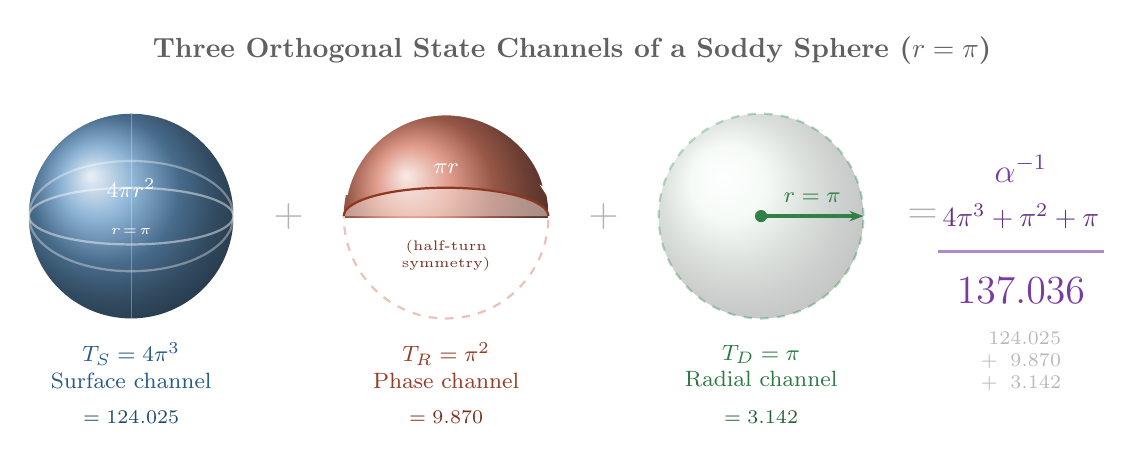
\begin{tikzpicture}[font=\small]
  \definecolor{col1}{RGB}{52,120,180}
  \definecolor{col2}{RGB}{200,80,50}
  \definecolor{col3}{RGB}{60,160,90}
  \definecolor{sumcol}{RGB}{120,60,160}

  % Sphere 1: Surface
  \begin{scope}[xshift=0cm]
    \shade[ball color=col1!75!white] (0,0) circle (1.3cm);
    \draw[white,opacity=0.45,thick] (0,0) ellipse (1.3cm and 0.36cm);
    \draw[white,opacity=0.35,thick] (0,0) ellipse (1.3cm and 0.7cm);
    \draw[white,opacity=0.30] (0,-1.3)--(0,1.3);
    \node[white,font=\bfseries\footnotesize] at (0,0.35) {$4\pi r^2$};
    \node[white,font=\tiny] at (0,-0.2) {$r\!=\!\pi$};
    \node[col1!75!black,font=\footnotesize,align=center] at (0,-1.9)
      {$T_S = 4\pi^3$\\\footnotesize Surface channel};
    \node[col1!60!black,font=\scriptsize] at (0,-2.55) {$=124.025$};
  \end{scope}

  \node[font=\Large\bfseries,gray!60] at (2.0,0) {$+$};

  % Sphere 2: Phase
  \begin{scope}[xshift=4.0cm]
    \begin{scope}
      \clip (-1.3,-0.02) rectangle (1.3,1.35);
      \shade[ball color=col2!75!white] (0,0) circle (1.3cm);
    \end{scope}
    \fill[col2!15!white,opacity=0.5]
      (-1.3,0) arc(180:0:1.3cm and 0.36cm) -- cycle;
    \draw[col2!70!black,thick]
      (-1.3,0) arc(180:0:1.3cm and 0.36cm);
    \begin{scope}
      \clip (-1.35,-1.35) rectangle (1.35,0);
      \draw[col2!35!white,dashed,thick] (0,0) circle (1.3cm);
    \end{scope}
    \draw[white,very thick,-{Stealth[length=4pt]}]
      ({1.3*cos(168)},{1.3*sin(168)}) arc(168:12:1.3cm);
    \node[white,font=\bfseries\footnotesize] at (0,0.6) {$\pi r$};
    \node[col2!60!black,font=\tiny,align=center] at (0,-0.5)
      {(half-turn\\symmetry)};
    \node[col2!75!black,font=\footnotesize,align=center] at (0,-1.9)
      {$T_R = \pi^2$\\\footnotesize Phase channel};
    \node[col2!60!black,font=\scriptsize] at (0,-2.55) {$=9.870$};
  \end{scope}

  \node[font=\Large\bfseries,gray!60] at (6.0,0) {$+$};

  % Sphere 3: Radial
  \begin{scope}[xshift=8.0cm]
    \draw[col3!40!white,dashed,thick] (0,0) circle (1.3cm);
    \shade[ball color=col3!18!white,opacity=0.35] (0,0) circle (1.3cm);
    \draw[col3!80!black,very thick,-{Stealth[length=5pt]}]
      (0,0) -- (1.3,0);
    \node[col3!80!black,font=\footnotesize\bfseries,above] at (0.65,0.05)
      {$r=\pi$};
    \fill[col3!80!black] (0,0) circle (2.2pt);
    \node[col3!75!black,font=\footnotesize,align=center] at (0,-1.9)
      {$T_D = \pi$\\\footnotesize Radial channel};
    \node[col3!60!black,font=\scriptsize] at (0,-2.55) {$=3.142$};
  \end{scope}

  % Equals + Sum
  \node[font=\Large\bfseries,gray!60] at (10.05,0) {$=$};
  \begin{scope}[xshift=11.3cm]
    \node[sumcol,font=\large\bfseries] at (0,0.6) {$\alpha^{-1}$};
    \node[sumcol!85!black,font=\normalsize] at (0,-0.0)
      {$4\pi^3+\pi^2+\pi$};
    \draw[sumcol!60,thick] (-1.05,-0.45)--(1.05,-0.45);
    \node[sumcol,font=\Large\bfseries] at (0,-0.95) {$137.036$};
    \node[gray!55,font=\scriptsize,align=right] at (0,-1.85)
      {$124.025$\\$+\;\;9.870$\\$+\;\;3.142$};
  \end{scope}

  \node[font=\normalsize\bfseries,gray!75!black] at (5.6,2.1)
    {Three Orthogonal State Channels of a Soddy Sphere ($r=\pi$)};
\end{tikzpicture}
\caption{The fine-structure constant $\alpha^{-1}$ as a sum of three orthogonal
  Presburger information costs for a single Soddy sphere of radius $r=\pi$.
  \textbf{Blue} ($T_S=4\pi^3$): surface-area channel.
  \textbf{Red} ($T_R=\pi^2$): phase channel (hemisphere only).
  \textbf{Green} ($T_D=\pi$): radial channel.
  No free parameters; $r=\pi$ is the unique Presburger-minimal radius (Axiom P2).}
\label{fig:alpha_channels}
\end{figure}




\begin{samepage}
\begin{center}
\begin{mdframed}
\textbf{Register interpretation.}
The inverse fine-structure value derived here is the full dimensionless Presburger computation cost of one finite Soddy-sphere register update:
\begin{align*}
T_{\rm sphere}
&= T_S+T_R+T_D \\
&=4\pi^3+\pi^2+\pi \\
&=137.0363038\ldots .
\end{align*}
The three costs are added because the FTC update is a sequential finite trace: the surface address, rotational phase, and radial displacement channels must each be resolved once in the causal order of a complete update. The cost counts finite causal work performed by the register, channel by channel, under Presburger-valid operations.

Exponential stability requires this finite trace to be recursively clampable. Each layer must complete its finite update before its output is used as input by the next layer. The resulting register depth near \(137\) is the exponential causal depth of a stable async sphere-register transaction inside the FTC.
\end{mdframed}
\end{center}
\end{samepage}

\subsubsection{Unique Accepting Alignment and Coupling Probability: $\alpha$}
\label{sec:alpha_deriv}

The single-sphere register derived above gives the full causal update depth
\[
T_{\rm sphere}=4\pi^3+\pi^2+\pi=137.0363038\ldots .
\]
This is the ontology-internal ASSP register value: the number of internally distinguishable causal micro-positions in one complete Soddy-sphere update, preserving the ordered surface channel, the hemisphere-restricted rotational phase channel, and the radial displacement channel simultaneously.

The FTC has no external synchronizing clock. Neighboring ball-registers update asynchronously. A mutual tangent interaction computes when adjacent registers are updated in the required mutual sequence during the complete update trace. An elementary electromagnetic transaction is the successful phase-aligned causal handshake between two adjacent Soddy registers: one register emits or presents a boundary phase defect, and the neighboring register accepts it in the causally ordered phase position compatible with the full single-sphere update.

\paragraph{Lemma: Unique accepting alignment.}

For a two-ball electromagnetic transaction, the number of accepting alignments is

\[
N_{\rm accept}=1.
\]

A successful adjacent-register handshake must close the surface, rotational-phase, and radial-displacement channels in the same causal order. Any offset in the receiving register breaks the full two-ball transaction. Among the \(T_{\rm sphere}\) internally distinguishable causal positions of the receiving register, exactly one position accepts the incoming boundary phase defect.

The elementary coupling probability is the finite-state counting probability for a unique accepting alignment inside a register with \(T_{\rm sphere}\) possible causal positions:

\[
P_{\rm align}
=
\frac{N_{\rm accept}}{N_{\rm possible}}
=
\frac{1}{T_{\rm sphere}}.
\]

Since the electromagnetic channel is defined in the ontology as adjacent-register phase transfer, the fine-structure constant is the elementary alignment probability:

\[
\boxed{
\alpha
=
P_{\rm align}
=
\frac{1}{T_{\rm sphere}}
=
\frac{1}{4\pi^3+\pi^2+\pi}
}
\]

or equivalently

\[
\boxed{
\alpha^{-1}
=
T_{\rm sphere}
=
4\pi^3+\pi^2+\pi
=
137.0363038\ldots
}
\]

Thus \(\alpha^{-1}\) is the full causal register depth of one complete Soddy-sphere update, while \(\alpha\) is the probability that an asynchronous neighboring register lands in the unique accepting alignment required for an elementary electromagnetic transaction. The identification of \(P_{\rm align}\) with \(\alpha\) is deductive inside the ontology: electromagnetism has already been defined as adjacent-register phase transfer, and \(\alpha\) is the elementary probability for such transfer.

\paragraph{Physical interpretation.}

The inverse fine-structure constant measures the full causal throughput cost for one complete Presburger tick of a single Soddy sphere:

\[
\alpha^{-1}
=
T_{\rm sphere}.
\]

This throughput cost includes surface specification, rotational phase, and radial displacement. An electromagnetic interaction is the adjacent-register phase-transfer transaction between two causally neighboring spheres. Because the transaction has exactly one accepting alignment among \(T_{\rm sphere}\) possible internal causal positions, its elementary throughput probability is

\[
\alpha
=
\frac{1}{T_{\rm sphere}}.
\]

The value derived here is the ontology-internal ASSP register value, compared against the CODATA recommended least-squares value of \(\alpha\)~\cite{CODATA2022}. Effective low-energy determinations of \(\alpha\) may differ between experimental channels because each atom realizes the electromagnetic register through a different evolved local configuration. This distinction is important because the present atom-recoil situation is unresolved: high-precision atom-recoil determinations using cesium and rubidium differ at the several-sigma level. The 2018 cesium measurement gave

\[
\alpha^{-1}_{\rm Cs}
=
137.035999046(27),
\]

while the 2020 rubidium measurement gave

\[
\alpha^{-1}_{\rm Rb}
=
137.035999206(11).
\]

The rubidium result was reported as differing by more than five standard deviations from the best cesium-recoil result~\cite{Parker2018,Morel2020}. No experimental error or systematic correction large enough to remove this discrepancy has been identified in the more than five years since the cesium result and the subsequent rubidium measurement.

Therefore, throughout this paper,

\[
\alpha_{\rm ASSP}^{-1}
=
4\pi^3+\pi^2+\pi
\]

is the predicted ASSP coupling-register depth used for comparison with laboratory determinations.


\subsection{The Fractal Quine: Two Balls and the Universal Fundamental Law}
\label{sec:quine}

The result $T_{\rm sphere} = 137.036$ is the complete description of a single isolated Soddy sphere. When a second sphere is placed in tangency with the first, the system becomes a self-executing program---the \textbf{fractal quine}:

\begin{enumerate}
  \item The first sphere (star ball) encodes angular momentum state into its surface channel $T_S = 4\pi^3$.
  \item Tangency with the second sphere (core ball) provides the unique Möbius-invariant coupling.
  \item The angular-and-linear momentum transfer in the higher fractal layer is the photonic mechanism (info ball).
  \item The computational cost is paid by injecting momentum  into the lower fractal layer (dust balls).
\end{enumerate}

\begin{quote}
One ball on top of $T_{\rm sphere} = 137.036$ is a state. Two balls in tangency is a law.
\end{quote}


\subsection{Two-Ball Computational Overhead and the Laderman 3x3 Split}
\label{sec:laderman_split}

When two balls form a gyro ball, the FTC promotes a one-register Presburger update into a three-channel Euclidean tangency update. The tangent balls are geared rotational computers. A true two-ball tangency update is therefore a finite geared-rotation computation across the three surface/phase/radial channels.

Fast matrix multiplication supplies the finite compute-count model: a higher-dimensional operation can be performed with fewer multiplication-like steps by paying additional addition-like bookkeeping. Strassen is mentioned only as the historical $2\times2$ prototype; the FTC uses Laderman's $3\times3$ multiplication scheme, which reduces the naive $27$ multiplication count to $23$ multiplication-like operations~\cite{Laderman1976}.

In the FTC interpretation, $23/27$ is the geared-rotation compute fraction of a three-channel tangent-ball update, while $4/27$ is the addition-only leakage complement. The rank-23 split is therefore used as the finite rotation-compute split of the gyro-ball boundary:

\begin{itemize}
  \item Naive $3\times3$: 27 multiplication-like operations.
  \item Laderman $3\times3$: 23 multiplication-like operations.
  \item Curvature fraction: $23/27 \approx 0.8519$.
  \item Addition-only leakage fraction: $4/27 \approx 0.1481$.
  \item Two-ball curvature overhead: $2 \times 23/27 \approx 1.7037$.
  \item Dual-channel leakage overhead: $2(23/27)^2(4/27) \approx 0.2150$.
  \item Total two-ball overhead: $\Delta T_{\rm two\text{-}ball} \approx 1.9187$.
\end{itemize}

Thus the two-ball quine depth is
\begin{equation}
\boxed{
T_{\rm two\text{-}ball}
=
T_{\rm sphere}+\Delta T_{\rm two\text{-}ball}
=
137.0363+1.9187
=
138.9550
}
\label{eq:138}
\end{equation}

The first cross-check of the two-ball register scale is the observed electron-to-solar logarithmic hierarchy:
\[
\ln(M_\odot/m_e)_{\rm obs} \approx 138.9357~\cite{CODATA2022},
\]
which lies close to the internally derived value \(T_{\rm two\text{-}ball}=138.9550\). The following section does not solve for the mass register from this observed hierarchy. Instead, it derives the 77-layer Star Ball self-encoding register from the rank-23 boundary split and then treats the electron--star hierarchy as a confirmation of the ontology.

% ==================================================================
%  MASS REGISTER AND STAR/ELECTRON HIERARCHY
% ==================================================================

\section{The Mass Register and the Electron--Star Hierarchy}


\subsection{Rank-23 Channel Split, Half-Boundary Register, and 77-Layer Encoding}
\label{sec:mass_channel}

The mass hierarchy is the quine self-encoding layer count of a Star Ball mass register consisting of the full single-sphere state plus one half of the rank-23 curvature boundary needed to define that state relationally. In our universe, the quantized-energy object and the flat-rotation-curve object are identified as fractal-equal objects constructed by their constituents: the electron and the star. The electron-to-solar hierarchy is therefore a cross-check: it tests whether the internal closure lands near the expected astrophysical scale.

\subsubsection{The Natural Split from Rank-23 Geometry}
\label{sec:natural_split}

The isolated single-ball register is
\[
T_{\rm sphere}^{\rm TFOFT}
=
4\pi^3+\pi^2+\pi
=
137.0363038.
\]
This is the complete FTC state cost of one isolated Soddy sphere.
However, a mass hierarchy is not a free-standing isolated sphere. A Star Ball
mass register only becomes a physical register when it is relationally
defined against a Core Ball boundary. The relevant construction is therefore
not the full two-ball transfer register, but the one-register mass channel
with a shared relational boundary.

The rank-23 two-ball geometry supplies the raw dual-channel leakage into the
Info Ball channel:
\[
k_{\rm info}^{(0),{\rm TFOFT}}
=
2\left(\frac{23}{27}\right)^2\left(\frac{4}{27}\right).
\]
Here \(23/27\) is the rank-23 curvature fraction relative to the naive
\(3\times3\) multiplication count, \(4/27\) is the addition-only leakage
fraction, and the prefactor of \(2\) counts the two directed boundary legs of
the Core--Star transfer. Numerically,
\[
k_{\rm info}^{(0),{\rm TFOFT}}
=
2\left(\frac{23}{27}\right)^2\left(\frac{4}{27}\right)
=
0.2150079.
\]

Within the \(e\)-clamped two-channel budget, the complementary mass step is
therefore
\[
k_{\rm mass}^{\rm TFOFT}
=
2-k_{\rm info}^{(0),{\rm TFOFT}}
=
1.7849921.
\]
This value is derived from the rank-23 channel geometry. It is not obtained
from \(\ln(M_\odot/m_e)_{\rm obs}\), from Karlsson periodicity, or from any
observed mass ratio.

\begin{quote}
The raw rank-23 geometry first determines the Info Ball leakage
\(k_{\rm info}^{(0),{\rm TFOFT}}\). The mass-channel step
\(k_{\rm mass}^{\rm TFOFT}\) is then the complementary \(e\)-clamped channel.
Observation may later check this value, but it does not define it.
\end{quote}

\subsubsection{Why 77 Layers: The Half-Boundary Mass Register}
\label{sec:why_77_layers}

The 77-layer count follows from the half-boundary Star Ball mass register and the rank-23 geared-rotation channel split. The Star Ball mass hierarchy is a one-register hierarchy that still requires a relational Core Ball boundary. The mass register therefore sits between the isolated single-ball state and the full two-ball quine transfer.

The lower limit is the isolated sphere:
\[
T_{\rm lower}^{\rm TFOFT}
=
T_{\rm sphere}^{\rm TFOFT}
=
137.0363038.
\]
The full two-ball boundary would add a complete rank-23 curvature boundary:
\[
T_{\rm upper}^{\rm TFOFT}
=
T_{\rm sphere}^{\rm TFOFT}
+
\left(\frac{23}{27}\right)
=
137.8881556.
\]
But the Star Ball mass register receives only half of this boundary, because
the boundary is shared relationally between the Star Ball and the Core Ball.
Thus the mass register is
\[
T_{\rm mass}^{\rm TFOFT}
=
T_{\rm sphere}^{\rm TFOFT}
+
\frac12\left(\frac{23}{27}\right).
\]
Numerically,
\[
T_{\rm mass}^{\rm TFOFT}
=
137.0363038
+
0.4259259
=
137.4622297.
\]

The self-encoding layer count is then the mass-register depth divided by the
internally derived mass-channel step:
\[
S_{\rm mass}^{\rm TFOFT}
=
\frac{T_{\rm mass}^{\rm TFOFT}}{k_{\rm mass}^{\rm TFOFT}}
=
\frac{137.4622297}{1.7849921}
=
77.00999
\approx
\boxed{77}.
\]

This is the central mass-hierarchy derivation. The integer \(77\) is selected
by the half-boundary Star Ball mass register and the rank-23 channel split
alone. No observed mass ratio is used to solve for \(k_{\rm mass}^{\rm TFOFT}\)
or \(S_{\rm mass}^{\rm TFOFT}\).

\begin{quote}
A single isolated sphere is a state. A full two-ball register is the quine
transfer. The mass hierarchy sits between them: it is the Star Ball's own
single-sphere state plus one half of the shared rank-23 curvature boundary.
That half-boundary closure pins the self-encoding count at
\(S_{\rm mass}^{\rm TFOFT}\approx77\).
\end{quote}

\subsubsection{Interval View of the Mass Register}
\label{sec:mass_interval_view}

The half-boundary construction places the mass register between the isolated
single-ball limit and the full two-ball boundary limit:
\[
T_{\rm sphere}^{\rm TFOFT}
<
T_{\rm mass}^{\rm TFOFT}
<
T_{\rm sphere}^{\rm TFOFT}+\frac{23}{27}.
\]
Equivalently, in layer units,
\[
\frac{T_{\rm sphere}^{\rm TFOFT}}{k_{\rm mass}^{\rm TFOFT}}
=
76.7714,
\]
\[
\frac{T_{\rm mass}^{\rm TFOFT}}{k_{\rm mass}^{\rm TFOFT}}
=
77.0100,
\]
\[
\frac{T_{\rm sphere}^{\rm TFOFT}+\frac{23}{27}}
{k_{\rm mass}^{\rm TFOFT}}
=
77.2486.
\]
Thus \(77\) is not selected by the lower isolated-sphere limit or by the upper
full two-ball transfer. It is selected by the half-boundary mass register.


\begin{figure}[h]
\centering
\resizebox{0.95\textwidth}{!}{%
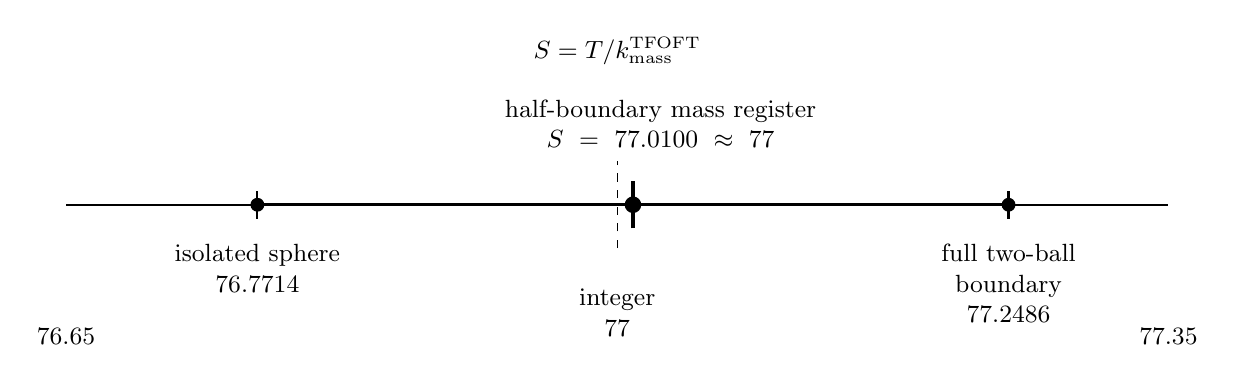
\begin{tikzpicture}[font=\small, x=1cm, y=1cm]

  % Horizontal axis: 76.65 to 77.35 mapped manually to 0..14
  \draw[thick] (0,0) -- (14,0);

  % x = (S - 76.65) / 0.70 * 14
  \coordinate (single) at (2.43,0);
  \coordinate (mass)   at (7.20,0);
  \coordinate (full)   at (11.97,0);
  \coordinate (int77)  at (7.00,0);

  % Interval
  \draw[very thick] (single) -- (full);

  % Markers
  \draw[thick] (2.43,-0.18) -- (2.43,0.18);
  \fill (single) circle (2.5pt);

  \draw[very thick] (7.20,-0.30) -- (7.20,0.30);
  \fill (mass) circle (3pt);

  \draw[thick] (11.97,-0.18) -- (11.97,0.18);
  \fill (full) circle (2.5pt);

  % Integer 77 reference
  \draw[dashed] (7.00,-0.55) -- (7.00,0.55);

  % Labels
  \node[align=center, text width=3.2cm, below=0.38cm] at (2.43,0)
    {isolated sphere\\$76.7714$};

  \node[align=center, text width=4.4cm, above=0.60cm] at (7.55,0)
    {half-boundary mass register\\$S=77.0100\approx77$};

  \node[align=center, text width=3.4cm, below=0.38cm] at (11.97,0)
    {full two-ball\\boundary\\$77.2486$};

  \node[align=center, below=0.95cm] at (7.00,0)
    {integer\\$77$};

  % Axis labels
  \node[below=1.45cm] at (0,0) {$76.65$};
  \node[below=1.45cm] at (14,0) {$77.35$};
  \node[above=1.65cm] at (7,0)
    {$S=T/k_{\rm mass}^{\rm TFOFT}$};

\end{tikzpicture}%
}
\caption{Mass-register interval in layer units. The half-boundary Star Ball
mass register gives \(S_{\rm mass}^{\rm TFOFT}=77.0100\approx77\), between
the isolated single-sphere limit and the full two-ball boundary.}
\label{fig:mass_register_interval}
\end{figure}

\subsubsection{Observed Electron-to-Solar Hierarchy}
\label{sec:mass_observed_crosscheck}

The observed electron-to-solar logarithmic hierarchy is
\[
N_{\rm mass}^{\rm obs}
=
\ln(M_\odot/m_e)_{\rm obs}
\approx
138.936.
\]
Using the integer closure \(S_{\rm mass}^{\rm TFOFT}\approx77\), the
corresponding observed effective step is
\[
k_{\rm mass}^{\rm obs}
=
\frac{N_{\rm mass}^{\rm obs}}{77}
\approx
1.80436.
\]
The TFOFT mass-channel step is
\[
k_{\rm mass}^{\rm TFOFT}=1.7849921,
\]
giving
\[
\frac{k_{\rm mass}^{\rm obs}-k_{\rm mass}^{\rm TFOFT}}
{k_{\rm mass}^{\rm TFOFT}}
\approx
1.1\%.
\]
This offset is comparable in role to the local virial and density corrections
appearing in the \(G\) and \(\alpha(Z)\) sections.


\subsubsection{The 137 $-$ 77 $=$ 60 Residual: He and Fe as Fractal Garbage Collectors}
\label{sec:he_fe_garbage_collector}

The nearest integer to the single-sphere register depth minus the derived
integer mass closure leaves the residual
\[
\lfloor\alpha_{\rm TFOFT}^{-1}\rfloor
-
S_{\rm mass}^{\rm TFOFT}
=
137-77
=
\boxed{60}.
\]

We conjecture that this residual encodes the \emph{fractal register garbage
collector}: the computational cost of closing the fractal circuit and
recycling the momentum debt incurred by mass-channel self-encoding. Persistent
computation requires a mechanism to restart fusion processes after a star has
exhausted its fuel. The residual Soddy core budget is conjectured to encode
the primary fusion endpoints:

\begin{itemize}
  \item \textbf{Helium-4 (\(A=4\))}: The tetrahedral Soddy-closed shell at
  four nucleons is conjectured to be the most stable arrangement of simple
  nucleons in the ASSP. Stability would arise because the external virtual
  Soddy density exceeds the internal virtual Soddy density, creating a net
  inward restoring force at every face of the tetrahedron.

  \item \textbf{Iron-56 (\(A=56\))}: The maximum nucleus for which synthesis
  still releases energy. Beyond \(A=56\), outer Soddy cores are conjectured
  to accumulate real curvature faster than inner cores can balance them, and
  binding energy per nucleon decreases monotonically.
\end{itemize}

Together,
\[
4+56=60
=
\lfloor\alpha_{\rm TFOFT}^{-1}\rfloor
-
S_{\rm mass}^{\rm TFOFT}.
\]

\begin{quote}
The two dominant nuclear fusion endpoints---helium and iron---are conjectured
to be the Soddy-closed garbage-collector states encoded into the arithmetic of
fractal self-description: the light and heavy bookends of the 60-unit momentum
debt separating the single-sphere register depth from the mass self-encoding
layer count.
\end{quote}



\subsection{Electron and Proton Mass from Recursive Soddy Curvature}

The electron rest mass \(m_e\) and proton mass \(m_p\) emerge from the recursive curvature dynamics of the Apollonian--Soddy sphere packing starting with the fundamental radius \(r = \pi\).

Numerical Soddy recursion with frontier pruning (retaining the 20 highest-curvature spheres) produces the following evolution of the deepest registers:

\begin{center}
\begin{tabular}{lcc}
\toprule
Generation & max \(\ln k\) & luminous-weighted (\(\times 23/27\)) \\
\midrule
38     & 81.8579 & 69.7308 \\
\textbf{38.5 (interpolated)} & \textbf{82.9509} & \textbf{70.6602} \\
39     & 84.0439 & 71.5929 \\
77     & 167.1095 & 142.3525 \\
\bottomrule
\end{tabular}
\end{center}

The factor \(23/27 \approx 0.85185185\) is the luminous (mass-bearing) channel fraction. It corresponds to the Laderman rank-23 heavy, curvature-intensive portion of the two-ball gyro-ball interaction that builds persistent inertial registers. The complementary \(4/27\) channel is the low-cost Info Ball transfer.

At half-depth (Gen 38.5), the luminous-weighted deepest curvature is \(70.6602\). Doubling for the full cycle gives \(141.3204\), close to the internal two-ball quine depth \(T_{\rm two-ball} \approx 138.955\).

The Star Ball mass register sits at the natural \emph{half-boundary} position:
\[
T_{\rm mass} = 4\pi^3 + \pi^2 + \pi + \tfrac12 \left( \tfrac{23}{27} \right) = 137.4622297\ldots
\]

A stable Core Ball (proton) is manufactured as a Soddy composite. The ratio \(m_p / m_e \approx 1836.15\) satisfies
\[
1836.15 / 77 \approx 23.846.
\]
This lies near the rank-23 Laderman curvature overhead, with a residual of approximately \(3.7\%\) relative to \(23\). It is therefore treated as an approximate structural check on the claim that core manufacturing corresponds to one full mass-register cycle modulated by the dominant Soddy/Laderman factor, rather than as an exact derivation.

\textbf{Quine Closure Condition.} 
The recursive Soddy geometry, weighted by the luminous fraction \(23/27\), must internally reproduce the register depths of the fractal quine. This determines the emergent conversion factor \(\sigma\) (geometric register cost \(\to\) physical mass/energy) and fixes the base Star Ball mass \(m_e\) such that
\[
\ln\left(\frac{M_\odot}{m_e}\right)_{\rm TFOFT} \approx T_{\rm two-ball} \approx 138.955
\]
holds as an internal relation of the ASSP architecture.

Thus \(m_e\) (and \(m_p = 1836.15\, m_e\)) is derived purely from the recursive Soddy curvature structure under Presburger cost minimization with initial radius \(r = \pi\). No external laboratory mass measurement is required as a primary input for the ratios and hierarchies. All other constants of the theory (\(\alpha\), \(E_H\), \(G\), etc.) follow directly from this self-describing fractal quine.

\textbf{On absolute scale in laboratory units.} 
Because the ontology is strictly fractal, each scale has its own ``electron'' (Star Ball). The here-scale electron mass in laboratory units (0.511\,MeV) requires one overall scale anchor. Once this anchor is fixed, absolute masses in kg or MeV become derived predictions. The dimensionless ratios and register structure, however, remain fully internal and zero-parameter.


% ==================================================================
%  ATOMIC CLOCK-LOCKING
% ==================================================================

\section{Atomic Clock-Locking: Hydrogen, Kepler Scaling, and the Rydberg Ladder}


\subsection{Local \(c\) as the Spherical Register Radius/Update Scale}

The follow-up dynamics paper derives the coarse GR/QM limits from the same ball dynamics. The point needed here is the local meaning of \(c\): the speed of light is the radial update rate of the local spherical register. In one-register-tick units, \(c\) is numerically the radius/update scale of the sphere defining the local causal clock.

A bound Star Ball does not move at the full radial light-update rate. It locks to the Core Ball at the fractional rate fixed by the single-sphere electromagnetic register:
\[
v_{\rm lock}=\alpha c.
\]
Thus the lock velocity is a relation between balls: the Star Ball runs at one \(\alpha\)-fraction of the Core-defined light-radius update scale.

\subsection{Atom Base Energy: Deriving the Hydrogen Binding Energy}

The hydrogen atom is the low-scale Gyro Ball. The ball mapping is
\[
\text{Core Ball} \leftrightarrow \text{proton/nucleus},
\qquad
\text{Star Ball} \leftrightarrow \text{electron},
\]
\[
\text{Gyro Ball} \leftrightarrow \text{closed Star--Core round trip},
\qquad
\text{Info Ball} \leftrightarrow \text{photon in transport}.
\]
Binding appears when the Star Ball and Core Ball complete one stable Gyro-Ball loop. The completed loop stores the kinetic closure cost of the Star Ball at the lock speed \(v_{\rm lock}=\alpha c\):
\begin{equation}
E_{\rm atom}
=
\frac12 m_{\rm star}v_{\rm lock}^2
=
\frac{\alpha^2 m_{\rm star} c^2}{2}.
\label{eq:atom_base}
\end{equation}

At the atomic layer the Star Ball is the electron, so \(m_{\rm star}=m_e\), giving
\[
E_H = \frac{\alpha^2 m_e c^2}{2} \approx 13.606\ \text{eV}.
\]

This is the ball-register origin of the hydrogen binding energy: local spherical radius/update scale gives \(c\), the single-sphere register gives \(\alpha\), and the completed Star--Core Gyro loop gives the stored binding energy.

\subsection{Kepler's Third Law as the Gyro Ball Clock-Locking Equation}
\label{sec:kepler_clock}

The Gyro Ball interpretation applies not only to the atomic hydrogen binding channel but also to the macroscopic orbital clock of a star around a core. Newton's form of Kepler's third law is~\cite{Newton1687}
\[
T^2=\frac{4\pi^2}{GM}a^3,
\]
where \(T\) is the orbital period, \(a\) is the semi-major axis, and \(GM\)
is the gravitational parameter of the core.

Multiplying by the Presburger basis radius \(r=\pi\) gives
\[
\pi T^2
=
4\pi^3\frac{a^3}{GM}.
\]
Thus Kepler's third law can be written in the ASSP form
\[
\boxed{
\pi T^2
=
4\pi^3\mathcal{K}_a
}
\qquad
\text{where}
\qquad
\mathcal{K}_a=\frac{a^3}{GM}.
\]

This is not merely a rescaling of the period. In the FTC interpretation,
\(\pi T^2\) is the orbital clock expressed through the fundamental-radius
channel \(r=\pi\). The factor \(4\pi^3\) is the universal Soddy surface
register cost already appearing in the single-sphere state budget,
\[
T_S=4\pi^3.
\]
The remaining factor,
\[
\mathcal{K}_a=\frac{a^3}{GM},
\]
is the local Kepler divider.

The semi-major axis \(a\) defines the radius of the virtual Soddy sphere
enclosing the Gyro Ball orbit via the tangency chain connecting the Star Ball
to the Core Ball boundary. Under this interpretation \(a^3\) is the
radial-volume information register of that virtual sphere. The factor
\(GM\) is the core curvature-throughput rate: the processing strength of the
Core Ball boundary. Hence \(\mathcal{K}_a\) is the virtual Soddy sphere's
information load per unit core throughput.

Equivalently, \(\mathcal{K}_a\) is the local clock-divider of the orbital
system. A larger virtual Soddy sphere contains more orbital information
volume and therefore requires a slower locked output clock. A larger core
throughput \(GM\) processes that volume faster and shortens the orbital
period.

In this form, Kepler's law functions like a phase-locked loop in a physical
FPGA. The universal reference is the fundamental-radius channel \(r=\pi\).
The local oscillator is the visible Gyro Ball orbital period \(T\). The
divider is \(\mathcal{K}_a=a^3/GM\). A stable orbit is the locked output
clock of the system:
\[
\text{radius-channel reference}
\quad\longrightarrow\quad
\text{local Kepler divider}
\quad\longrightarrow\quad
\text{stable Gyro Ball clock}.
\]

Under this ontology, ordinary orbital time is not fundamental in the FTC.
It is the relative time generated when the luminous addition-only transfer
channel locks to the ASSP radius/surface register. The visible star orbit is
the \(\sim4/27\) addition-efficient channel of the two-ball update, while the
complementary \(\sim23/27\) Laderman rank-23 overhead is paid into lower-layer
substrate and appears as dark computational mass rather than luminous
Keplerian motion.

The connection to the fine-structure derivation is direct. The full
single-sphere register is
\[
T_{\rm sphere}=4\pi^3+\pi^2+\pi,
\]
where \(4\pi^3\) is the dominant surface channel. Kepler's third law isolates
this same leading surface channel and turns it into the observable relative
clock of a macroscopic Gyro Ball:
\[
\pi T^2 = 4\pi^3\mathcal{K}_a.
\]
Therefore \(\alpha^{-1}\) gives the full async single-sphere register depth,
while Kepler's law gives the radius-locked relative clock by which visible
Gyro Balls execute their luminous orbital updates.


\subsection{Rydberg Scaling from Virtual-Core Clock Quantization}
\label{sec:rydberg_virtual_core}

The FTC does not quantize free orbits. A Star Ball may evolve continuously
under the Gyro Ball Kepler clock until the tangency chain reaches a
Core--Star boundary. Quantization enters only at the boundary-transfer
event, where the angular-momentum component of the update is copied into
an Info Ball channel.

The reason the transfer is quantized is that the Core Ball is not a
continuum object. In the FTC ontology, a Core Ball is a virtual
boundary-throughput object defined by finite ASSP support around a stable
tangency center. That support may be supplied by luminous Star Balls, by
Dust Balls and lower-layer substrate, by sub-stellar objects, or by any
combination of these channels. A galaxy core with many visible stars is one
realization; a dark-matter-dominated or star-free core is another. Such a
``naked'' Core Ball is still physically real in the FTC sense if its
boundary condition is maintained by lower-layer tangency pressure and
substrate flow.

At the galactic scale, the luminous Star Ball population contributes to the
center-of-mass and visible Kepler clock of the Core Ball, but it need not
supply the whole definition. The remaining support may be carried by Dust
Balls, sub-stellar objects, and lower-layer substrate. At the atomic scale,
the proton/nuclear core is the corresponding lower-scale Core Ball, while
the electron is the Star Ball. The observed atomic clock is therefore a
fractal Kepler clock: ordinary atomic time is the lower-scale analogue of
the macroscopic Gyro Ball orbital clock.

From the radius-channel Kepler relation derived above,
\[
\pi T^2
=
4\pi^3\mathcal{K}_a,
\]
the quantity \(\pi T^2\) is the orbital clock expressed through the
fundamental-radius channel \(r=\pi\). It is the internal ASSP clock-cost of
the virtual Core--Star system. Photon frequency is the inverse clock output,
so boundary-transfer energy is controlled by inverse clock-area:
\[
E\propto\frac{1}{T^2}.
\]

Let \(n\) denote the integer virtual-core clock layer defined by the finite
ASSP support of the Core Ball. This support need not be luminous. It may be
provided by Star Balls, Dust Balls, sub-stellar registers, lower-layer gas,
or any mixture of these components. Thus \(n\) is not a Bohr orbit quantum
number and not merely a count of visible orbiting bodies. It is the number
of completed Kepler-supported or substrate-supported clock layers available
to the virtual Core Ball at the boundary-transfer event.

Because the target Info Ball channel must be written into a completed ASSP
ball layer, only integer \(n\) is allowed. There is no half-layer write
target. The \(n\)-th virtual-core clock layer satisfies
\[
T_n=nT_1.
\]
Therefore its inverse clock-area is
\[
\frac{1}{T_n^2}
=
\frac{1}{n^2T_1^2}.
\]

The base Core--Star boundary-transfer energy is the Gyro Ball energy
\[
E_{\rm atom}
=
\frac{\alpha^2m_{\rm star}c^2}{2}.
\]
Thus the allowed boundary energies are
\[
\boxed{
E_n
=
-\frac{E_{\rm atom}}{n^2}.
}
\]

For hydrogen, \(m_{\rm star}=m_e\), so
\[
E_{\rm atom}=13.606\,{\rm eV},
\]
and
\[
E_n=-\frac{13.606\,{\rm eV}}{n^2}.
\]
A photon is emitted when the virtual Core Ball relocks from one completed
clock layer to another:
\[
E_\gamma
=
E_{\rm atom}
\left(
\frac{1}{n_f^2}
-
\frac{1}{n_i^2}
\right).
\]

Thus the Rydberg \(1/n^2\) law is not imposed by quantized free orbits.
It follows from the inverse-square clock-area of a finite virtual Core Ball:
the Kepler relation defines ASSP internal time, and discrete ball-layer
support quantizes the clock layers at the Core--Star boundary. The emitted
Info Ball carries the angular-momentum part of the relocking event, while
the complementary linear-momentum cost remains behind in lower-layer
substrate. 

\subsubsection{Finite Lyman and Rydberg Ceilings}

The two-ball quine depth provides two distinct spectral ceilings. The direct
basis-channel transfer, corresponding to the Lyman series \(n_i\to1\), is
limited by the two-ball boundary depth itself:
\[
n_{\max}^{\rm Lyman}
\sim
T_{\rm two\text{-}ball}
\approx139.
\]
This is the maximum direct Core--Star boundary relocking depth into the
basis hydrogen register.

At this depth, the last direct Lyman transfer lies only
\[
\frac{13.606\,{\rm eV}}{139^2}
\approx
7.04\times10^{-4}\,{\rm eV}
\]
below the conventional infinite-\(n\) Lyman limit. Adjacent terminal
Lyman-line spacing near this depth is approximately
\[
\Delta E
\sim
\frac{2(13.606\,{\rm eV})}{139^3}
\approx
1.0\times10^{-5}\,{\rm eV}.
\]
Therefore ordinary spectroscopy would see the finite basis-channel ceiling
as an effective continuum edge unless the experiment resolves sub-meV
structure near the Lyman limit and controls broadening effects.

Rydberg-like configurations are different. They are not direct relockings
into the basis state but composite excited tangency-chain configurations
inside the rotational channel. Since the rotational channel has quadratic
subdivision, the effective composite hydrogen address-space ceiling scales
as
\[
n_{\max}^{\rm H}
\sim
\left(T_{\rm two\text{-}ball}\right)^2
\approx
139^2
\approx
1.93\times10^4.
\]
This number should be interpreted as the number of principal hydrogen
register addresses, not the number of pairwise emitted lines. Spectral
lines are relockings between finite register addresses. Therefore the full
transition graph can contain many pairwise differences, but it remains
finite because the underlying hydrogen register has only finitely many
allowed address states.

Thus the FTC does not predict the absence of high-\(n\) Rydberg states above
\(n\approx139\). It predicts that the direct Lyman basis-channel transfer
saturates near \(n\approx139\), while composite Rydberg states can extend
to the quadratic rotational-channel ceiling.





\subsection{Nuclear Binding Energy: The Soddy Fractal Nucleon Stack}

\subsubsection{The Soddy Core Concept}

In any Apollonian-Soddy sphere packing, a cluster of $n$ mutually tangent equal spheres admits:
\begin{itemize}
  \item An \textbf{inner Soddy sphere} fitting exactly in the central interstice (positive curvature, bending inward).
  \item A \textbf{virtual outer Soddy sphere} circumscribing the cluster (negative curvature, bending outward).
\end{itemize}
Both are determined uniquely by the Descartes--Soddy relation~\cite{Soddy1936,Boyd1973,Graham2003}.

\subsubsection{Four Nucleons: The Tetrahedral Peak}

The minimal 3D Soddy-balanced configuration is four mutually tangent equal spheres arranged in a regular tetrahedron. For this configuration, both inner and outer Soddy cores remain virtual, acting as geometric pressure-balance constraints. The tetrahedral four-nucleon cluster is conjectured to experience maximum restoring force and minimal dislocatability---consistent with $^4$He having the highest binding energy per nucleon ($\approx 7.07$ MeV/nucleon) among light nuclei.

\subsubsection{Five Nucleons: First Inner Soddy Core Manifests}

Adding a fifth nucleon breaks the tetrahedral balance. The inner Soddy core becomes a resolvable packing site while the outer remains virtual. The asymmetric balance is conjectured to reduce binding energy per nucleon---consistent with the absence of stable $A=5$ nuclei in nature.

\subsubsection{The Iron Peak (Conjecture)}

Iron ($^{56}$Fe) is conjectured to sit at the global binding energy maximum ($\approx 8.79$ MeV/nucleon) because it is the first Soddy iteration at which both inner and outer Soddy cores are simultaneously real and balanced at the same iteration depth. Beyond $A=56$, outer Soddy cores are conjectured to accumulate real curvature faster than inner cores can balance them.


\subsection{Pauli Exclusion from Soddy Uniqueness (Conjecture)}

Given any interstice in a locally finite Apollonian-Soddy sphere packing, the corresponding tangent sphere is fixed by the Descartes--Soddy relation~\cite{Soddy1936,Boyd1973,Graham2003}. We conjecture that this geometric uniqueness is the physical origin of the Pauli exclusion principle.



% ==================================================================
%  BALL ONTOLOGY AFTER THE REGISTER AND ATOMIC BASIS
% ==================================================================
\section{The Ball Ontology: Fundamental Objects of the FTC}


As noted earlier, we use three scale prefixes throughout the ontology. \textbf{Atom} denotes the atomic scale. \textbf{Here} denotes the galactic/stellar scale. \textbf{Wish} denotes the scale above the galactic, where our galaxy plays the role that an atom plays at our scale.

The FTC basis begins with four primary objects. A \textbf{Star Ball} is the orbiting angular-momentum register: at the atomic scale it is the electron, and at the here-scale it is the star. A \textbf{Core Ball} is the receiving and emitting boundary register: at the atomic scale it is the proton/nucleus, and at the here-scale it is the galactic core. A Star Ball bound to a Core Ball forms a \textbf{Gyro Ball}, the closed Star--Core circuit: atom at the lower scale, spiral galaxy at the here-scale. An \textbf{Info Ball} is the photon/macrophoton in transport, the cross-scale angular-momentum carrier moving between source and receiver.

When the transport channel Info Ball lands at a Core boundary, the receiving side can recombine in two main ways. A lower-power coherent reconstruction produces a \textbf{Spit Ball}, identified astrophysically with black-hole or AGN jet behavior. A higher-power reconstruction produces a \textbf{Fast Ball}, identified astrophysically with quasars. Thus the table distinguishes the transport carrier from the receiving-side reconstruction: Info Ball is the photon/macrophoton in transport; Spit Ball and Fast Ball are post-injection recombination channels.

The remaining ball types name the supporting FTC bookkeeping objects. \textbf{Dust Balls} are the lower-scale linear-momentum cost paid by the transfer, appearing here-scale as dark-matter halo substrate which is the lower fractal scale interstellar medium (e.g, smaller scale hydrogen gas). \textbf{Pipe Balls} are elongated lower-layer tangency chains that behave as magnetic-field-line or filament channels. \textbf{Wake Balls} are the disturbance patterns generated by moving registers. \textbf{Roll, Spin, Kick, and Data Balls} describe the conservation bookkeeping of angular, linear, and internal state. These names are not independent new particles; they are the FTC vocabulary for the same recursive ASSP register dynamics viewed by role.


\begin{center}
\small
\renewcommand{\arraystretch}{1.35}
\begin{longtable}{|C{2.4cm}|L{6.2cm}|C{2.4cm}|C{3.0cm}|}
\caption{TFOFT Ball Ontology: the conjectured self-describing objects of the FTC. Cross-scale correspondences are proposed exact fractal-scale equivalences governed by the same Presburger equations with only scale parameters $r$ and mass $M$ varied.}
\label{tab:ball_ontology}\\
\hline
\textbf{Ball Type} & \textbf{Role in FTC} &
  \textbf{Atomic Equiv.} & \textbf{Astro.\ Equiv.} \\
\hline
\endfirsthead
\hline
\textbf{Ball Type} & \textbf{Role in FTC} &
  \textbf{Atomic Equiv.} & \textbf{Astro.\ Equiv.} \\
\hline
\endhead
\hline
\multicolumn{4}{r}{\textit{Continued on next page}}\\
\hline
\endfoot
\hline
\endlastfoot
Star Ball  & Orbiting angular-momentum register; the stable bound unit around a Core Ball. & Electron & Star \\
\hline
Core Ball  & Receiving and emitting boundary register; equator converts incoming angular momentum into outgoing lower-scale linear-momentum cost, while poles receive non-local Info-Ball transport. & Proton / Nucleus & Galactic core \\
\hline
Gyro Ball  & Star Ball bound to Core Ball; the closed Star--Core circuit for storage and transfer of angular and linear momentum. & Hydrogen atom & Spiral galaxy \\
\hline
Roll Ball  & Conservation bookkeeping object; comprised of Spin Ball, Kick Ball, and Data Ball components. & Lower-scale force bleed channels & Here-scale gravity and EM \\
\hline
Spin Ball  & Angular momentum carrier; rotational state component of Roll Ball. & Inertia & Inertia \\
\hline
Kick Ball  & Linear momentum carrier; translational state component of Roll Ball. & Motion & Motion \\
\hline
Data Ball  & Interior information state; ball state plus embedded data; chaotic lower-layer register beneath the primary sphere. & Interior atomic state & Interior stellar state \\
\hline
Wake Ball  & Fluid-like disturbance pattern generated by moving Roll Balls; propagates through the Soddy packing. & Quantum wave function & EM and gravitational waves \\
\hline
Info Ball  & Photon/macrophoton in transport: cross-scale angular-momentum information carried between source and receiver. Its transport is inferred from the receiving-side reconstruction state. & Photon in transport & Macrophoton in transport \\
\hline
Spit Ball  & Lower-power receiving-side recombination from an Info-Ball transport channel at a Core boundary; astrophysically expressed as coherent jet behavior. & Virtual particles; weak-force-like emission & Black-hole / AGN jet \\
\hline
Fast Ball  & Higher-power receiving-side recombination from an Info-Ball transport channel at a Core boundary; astrophysically observed as post-transport anti-core/anti-proton-like states. & Gamma-ray reconstruction & Quasar / anti-core candidate \\
\hline
Dust Ball  & Linear momentum computational cost exhausted to scale $A{-}1$ as lower-scale gyro-balls and constituents. & Electron cloud & Dark matter halos \\
\hline
Null Core  & Condensation of scattered lower-scale layers; regions of minimal Soddy packing density. & Galactic void centers & CMB cold spot \\
\hline
Code Ball  & Self-referential binding component enabling directed, coherent exchange at core boundaries. & Neutrinos & Life; planets; directed stellar processes \\
\hline
Pipe Ball  & Elongated Soddy tangency chain in lower fractal layer, oriented along angular momentum gradient. & Strong-force bookkeeping channel; lower-scale gravity bleed & Cosmic web filament \\
\hline
Jolt Ball  & Transient energy redistribution events at the scales between fractal layers. & Atomic decay & Local entropy spikes \\
\hline
Edge Ball  & Variable boundary where the dominant force regime changes. On Earth this transition is expected in the approximate \(0.1\)--\(2\,{\rm mm}\) range. & Planck-length analogue & \(0.1\)--\(2\,{\rm mm}\) wish-scale analogue \\
\hline

\end{longtable}
\normalsize
\end{center}

\subsection{Pipe Balls and Force Bleed Across Scale Boundaries}

A \textbf{Pipe Ball} is an elongated, quasi-one-dimensional chain of Soddy tangencies in the lower fractal layer, oriented along the gradient of the here-scale angular momentum field. It acts as the fractal-scale analogue of a magnetic field line: a low-density highway of lower-scale hydrogen substrate. In TFOFT, galactic-scale magnetic field lines are physical Pipe Balls tracing the angular-momentum gradient of the local ASSP. The inter-galactic filaments of the cosmic web are their here-scale manifestation at the wish-scale.

The four standard fundamental forces are interpreted as one FTC boundary force observed through different scale projections. The same causal boundary interaction bleeds across the upper and lower fractal scale boundaries in two directions. Here-scale electromagnetism and here-scale gravity are the visible force channels at our layer. The weak interaction is local electromagnetism expressed at the lower fractal scale. The strong interaction is local gravity expressed at the lower fractal scale. This explains why electromagnetic and weak behavior unify as electroweak behavior: they are adjacent-scale expressions of the same boundary channel. It also explains why the strong interaction behaves like an extreme confinement force: it is gravity viewed through the lower-scale Core-boundary geometry.

Gauge boson language remains useful as Standard Model transition bookkeeping. The FTC ontology assigns physical priority to boundary channels, scale crossing, and tangent-register dynamics. Photons remain Info Balls in transport because they are the observed cross-scale angular-momentum carriers. Gluons are treated as Standard Model internal labels for confinement bookkeeping, corresponding in TFOFT to lower-scale gravity-binding behavior inside the Core/Pipe channel, with no independent separable-object role.

\subsection{Charge, Direction, and Neutrality in the Particle Dictionary}

Charge records the direction of causal energy flow in the FTC:
\[
- \leftrightarrow \mathrm{emission/source/outward\ Star\ Ball\ channel},
\]
\[
+ \leftrightarrow \mathrm{absorption/sink/inward\ Core\ Ball\ channel},
\]
\[
0 \leftrightarrow \mathrm{neutral\ reservoir,\ closed\ loop,\ balanced\ composite,\ or\ neither\mbox{-}channel\ body}.
\]
Thus the electron is the basic emitting Star Ball channel, while the proton is the basic absorbing Core Ball channel. Neutral objects split into two cases. Some neutral channels are neither-side reservoirs, such as planets, substellar bodies, dust, and neutrino Code Balls. Other neutral channels are balanced composites or closed loops, such as neutron-like reservoirs, neutral weak handshakes, or neutral boundary pulses.

\subsection{Code Balls: Neutrino Flavor Channels as Sub-Stellar Lifecycle Stages}

The three neutrino flavor channels are compared with the passive substellar ladder using the same electron--star scaling rule:
\[
\frac{m_e}{m_\nu}
\leftrightarrow
\frac{M_\odot}{M_{\rm object}},
\]
so that
\[
M_{\rm object}=M_\odot\frac{m_\nu}{m_e}.
\]
Using \(m_e=510998.95069\,\mathrm{eV}\), a neutrino-channel mass \(m_\nu\) maps to an astronomical object whose mass is the same fraction of the Sun as \(m_\nu\) is of the electron.

The direct flavor-channel laboratory ceilings are
\[
m_{\nu_e}<0.45\,\mathrm{eV},
\]
from the KATRIN tritium endpoint result~\cite{KATRIN2025},
\[
m_{\nu_\mu}<0.19\,\mathrm{MeV},
\]
from direct pion-decay kinematic limits summarized by the Particle Data Group~\cite{PDG2024}, and
\[
m_{\nu_\tau}<18.2\,\mathrm{MeV},
\]
from the ALEPH tau-neutrino endpoint analysis~\cite{ALEPH1998TauNu}. These laboratory numbers are used as flavor-channel ceilings; the active mass eigenstates need not saturate them.

Representative substellar masses map to the following neutral-channel values:
\[
\mathrm{Mercury}:\quad 0.0553M_\oplus\Rightarrow m_\nu\approx0.085\,\mathrm{eV},
\]
\[
\mathrm{Mars}:\quad 0.107M_\oplus\Rightarrow m_\nu\approx0.164\,\mathrm{eV},
\]
\[
\mathrm{Neptune}:\quad 17.1M_\oplus\Rightarrow m_\nu\approx26.3\,\mathrm{eV},
\]
\[
\mathrm{Jupiter}:\quad 317.8M_\oplus\Rightarrow m_\nu\approx488\,\mathrm{eV},
\]
\[
13M_J:\quad m_\nu\approx6.34\,\mathrm{keV},
\]
\[
75M_J:\quad m_\nu\approx36.6\,\mathrm{keV}.
\]
The planetary values use standard Solar-System mass ratios~\cite{NASAPlanetaryFactSheet}. The brown-dwarf comparison uses the usual deuterium-burning scale near \(13M_J\) and the hydrogen-burning transition near \(75M_J\)~\cite{Spiegel2011}.

The resulting FTC channel alignment is
\[
\nu_e \leftrightarrow \mathrm{rocky/sub\mbox{-}Earth\ Code\ Ball},
\]
\[
\nu_\mu \leftrightarrow \mathrm{ice/gas\ giant\ Code\ Ball},
\]
\[
\nu_\tau \leftrightarrow \mathrm{brown\ dwarf\ and\ heavier\ neutral\ Code\ Ball}.
\]
No fourth light neutrino is expected because no fourth Soddy-stable passive substellar regime exists between the brown-dwarf channel and the active Star Ball regime~\cite{NuFIT2024}. The absence of a measured nonzero lower floor for the lightest neutrino channel mirrors the absence of a sharp lower floor in the substellar hierarchy: below the stellar threshold, the FTC ladder descends through brown dwarfs, gas giants, ice giants, rocky bodies, moons, dwarf planets, asteroids, dust, and lower-layer substrate.

\subsection{Standard Model Channels in the TFOFT Dictionary}

TFOFT assigns astronomical analogues to physically realized channels: emitters, absorbers, neutral code reservoirs, and boundary-transfer modes. Confined quark labels are treated as Standard Model coordinates for internal Core response. The Core Ball is an irreducible absorbing register at the atomic/galactic layer and has no same-layer decomposition into smaller observable cores.

\begin{center}
\small
\renewcommand{\arraystretch}{1.25}
\begin{longtable}{|C{2.2cm}|C{1.5cm}|L{4.3cm}|L{5.2cm}|}
\caption{Standard Model channel dictionary under the FTC ontology.}
\label{tab:sm_tfoft_dictionary}\\
\hline
\textbf{SM item} & \textbf{Charge} & \textbf{FTC status} & \textbf{Astronomical analogue} \\
\hline
\endfirsthead
\hline
\textbf{SM item} & \textbf{Charge} & \textbf{FTC status} & \textbf{Astronomical analogue} \\
\hline
\endhead
\hline
\multicolumn{4}{r}{\textit{Continued on next page}}\\
\hline
\endfoot
\hline
\endlastfoot
\(e^-\) & \(-1\) & Elementary emission channel & Star Ball / Sun-like emitter \\
\hline
\(e^+\) & \(+1\) & Reversed electron channel & Positron / stellar sink counterpart \\
\hline
\(\mu^-\) & \(-1\) & Overmassive emission channel, \(m_\mu/m_e\approx206.77\) & Very massive blue/WNh Star Ball \\
\hline
\(\tau^-\) & \(-1\) & Cluster-scale emission channel, \(m_\tau/m_e\approx3477.23\) & Compact proto-cluster / cluster-core emitter \\
\hline
\(p^+\) & \(+1\) & Irreducible Core Ball absorber & Galactic core / atomic core \\
\hline
\(\bar p\) & \(-1\) & Reversed Core Ball channel & Quasar / anti-core candidate \\
\hline
\(n^0\) & \(0\) & Neutralized Core Ball reservoir & Balanced core store \\
\hline
\(\gamma\) & \(0\) & Info Ball transfer channel & Photon / macrophoton transport \\
\hline
\(\nu_e\) & \(0\) & Neutral Code Ball channel & Rocky/sub-Earth channel \\
\hline
\(\nu_\mu\) & \(0\) & Neutral Code Ball channel & Ice/gas-giant channel \\
\hline
\(\nu_\tau\) & \(0\) & Neutral Code Ball channel & Brown-dwarf channel \\
\hline
\(W^-\) & \(-1\) & Weak emission-side boundary transition; lower-scale EM bleed & Outward decay boundary \\
\hline
\(W^+\) & \(+1\) & Weak absorption-side boundary transition; lower-scale EM bleed & Inward capture boundary \\
\hline
\(Z^0\) & \(0\) & Balanced weak boundary transition & Neutral weak handshake \\
\hline
\(H^0\) & \(0\) & Mass-register clamping excitation & Neutral mass-clamp mode \\
\hline
Quarks & fractional & Standard Model internal Core-response labels & No independent astronomical object \\
\hline
Gluons & color & Standard Model confinement bookkeeping; lower-scale gravity-binding channel & No independent separable object \\
\hline
\end{longtable}
\normalsize
\end{center}

\subsection{Decay Hints for the Charge-Direction Dictionary}

The Standard Model decay channels provide useful sign-flow hints for the FTC dictionary. Neutron beta decay,
\[
n^0\rightarrow p^+ + e^- + \bar\nu_e,
\]
reads as a neutral Core reservoir splitting into an absorbing Core channel, an emitting Star channel, and an escaping neutral Code channel.

Muon decay,
\[
\mu^-\rightarrow e^-+\bar\nu_e+\nu_\mu,
\]
reads as an overmassive emitting channel relaxing into the ordinary emitting channel plus neutral Code channels. Tau decays similarly express a cluster-scale emitting channel relaxing into lighter emitters, neutral Code channels, and composite Core fragments.

\subsection{Wave-Particle Duality as Fractal Pilot-Wave Dynamics (Conjecture)}

A Star Ball traversing the region near two adjacent Soddy interstices generates a \textbf{Wake Ball}: a fluid-like angular-momentum disturbance propagating through the ASSP fractal substrate. The interference pattern arises because the Wake Ball explores both interstice paths simultaneously.

% ==================================================================
%  FINE-STRUCTURE CONSTANT AND PREDICTIONS
% ==================================================================

\section{Fine-Structure Constant: Bare Register, Recoil Corrections, and Predictions}

\subsection{Electromagnetism as Local Boundary Realization}

In TFOFT, the fine-structure constant is not a universal abstract number
inserted into a Lagrangian. It is the local boundary realization of the
lower fractal scale. Thus \(\alpha\) is expected to be extremely stable
within a given register environment, but not absolutely universal across
distinct atomic, nuclear, and chiral boundary realizations.

This differs sharply from the standard QED ontology, in which \(\alpha\)
is a universal coupling and atomic recoil experiments are merely different
routes to measuring the same constant.

In TFOFT, the measured value is instead
\begin{equation}
\alpha_X^{-1}
=
\alpha_{\rm bare}^{-1}
+
\mathrm{boundary\ realization}
+
\mathrm{packing\ deformation}.
\end{equation}
The Rb/Cs/Yb recoil pattern is therefore not interpreted as experimental
scatter around a universal constant, but as the first visible evidence of
species-dependent boundary realization.

The corrected model predicts:
\begin{equation}
\alpha_X^{-1}
=
\alpha_{\rm reg}^{-1}
+
C_0^{\rm theory}
+
k\ln A
+
\lambda\Phi_{\rm bind}(A,Z).
\end{equation}

If future recoil measurements of Yb, Sr, Ca, or isotope series fail to
show this pattern, the TFOFT recoil model is falsified. If they do show
this pattern, then the standard interpretation of \(\alpha\) as a single
universal input parameter is falsified.



\subsection{Bare Register Depth Versus Physical Fine-Structure Coupling}

A central correction to the TFOFT interpretation is that the quantity
\begin{equation}
\alpha_{\rm reg}^{-1}
=
4\pi^3+\pi^2+\pi
=
137.036303775878\ldots
\end{equation}
must not be identified directly with the laboratory fine-structure
constant. Instead, this value represents the bare ASSP/Soddy/Presburger
register depth: the integer-plus-residual coupling depth before the first
physical dynamical object has formed.

The physical coupling is not realized by an isolated mathematical sphere.
It is realized only after the first star--core gyroball appears. Thus the
observed electromagnetic coupling is a boundary-realized quantity, not the
bare register itself.

Let
\begin{equation}
r = \alpha_{\rm reg}^{-1}-137.
\end{equation}
The integer floor \(137\) is the coarse register count, while \(r\) is the
fractional residual that must be dynamically discharged by the first
physical gyroball.

The first physical object is a two-pole star--core object rather than an isolated single sphere:
\begin{equation}
\mathrm{gyroball}=\mathrm{star}+\mathrm{core}.
\end{equation}
Therefore even hydrogen is not equal to the bare register value. Hydrogen
already contains a two-ball realization correction.

We define the theoretical hydrogen/gyroball correction
\begin{equation}
C_0^{\rm theory}
=
-
\frac{\alpha_{\rm reg}^{-1}-137}{137}
\cdot
\frac{27}{23+\phi^{-1}},
\end{equation}
where
\begin{equation}
\phi=\frac{1+\sqrt{5}}{2}.
\end{equation}

Numerically,
\begin{equation}
C_0^{\rm theory} = -0.000302936254\ldots
\end{equation}
and hence the physical hydrogen baseline becomes
\begin{equation}
\alpha_H^{-1}
=
\alpha_{\rm reg}^{-1}
+
C_0^{\rm theory}
=
137.036000839624\ldots .
\end{equation}

The factor \(23/27\) is interpreted as the gyroball's dynamical
self-encoding efficiency. It appears in the denominator because the
available register capacity is reduced by the shared-boundary efficiency,
so the same residual is distributed across fewer effective physical
registers. The \(\phi^{-1}\) term is the first golden-ratio correction
from the self-similar fractal packing geometry.

Thus the bare register is not the physical fine-structure constant.
The physical constant is the first realized gyroball projection of the
bare register.


\subsection{Binding-Energy Curve as a Higher-Order Soddy Packing Correction}

The minimal model
\begin{equation}
\alpha_X^{-1}
=
\alpha_{\rm reg}^{-1}
+
C_0^{\rm theory}
+
k\ln A
\end{equation}
captures the dominant nucleon-register depth. However, the nuclear binding
energy curve should appear as a higher-order local packing deformation.

We therefore write the next-order model as
\begin{equation}
\alpha_X^{-1}
=
\alpha_{\rm reg}^{-1}
+
C_0^{\rm theory}
+
k\ln A
+
\lambda\Phi_{\rm bind}(A,Z),
\end{equation}
where \(\Phi_{\rm bind}(A,Z)\) is a dimensionless measure of local nuclear
packing stability. A first candidate is
\begin{equation}
\Phi_{\rm bind}(A,Z)
=
\frac{B(A,Z)/A}{m_uc^2},
\end{equation}
where \(B(A,Z)/A\) is binding energy per nucleon. In fractal form:
\begin{equation}
\Phi_{\rm bind}(A,Z)
=
\left[
\eta
\frac{B(A,Z)/A}{m_uc^2}
\right]^{3/D_f},
\end{equation}
where \(D_f\approx2.47\) is the effective fractal dimension and
\(\eta\approx23/27\) is the gyroball packing efficiency.

The most important test is isotope dependence. For Yb isotopes,
\begin{equation}
^{168}{\rm Yb},\ ^{170}{\rm Yb},\ ^{171}{\rm Yb},\ ^{172}{\rm Yb},
\ ^{173}{\rm Yb},\ ^{174}{\rm Yb},\ ^{176}{\rm Yb},
\end{equation}
the \(\ln A\) term varies smoothly, while \(\Phi_{\rm bind}\) should
produce tiny isotope-specific residuals. Detection of such residuals would
be a strong signature that \(\alpha\) is a local boundary-realized
coupling rather than a universal external constant.


\subsection{Corrected Species-Dependent Recoil Model}

The corrected minimal recoil model is
\begin{equation}
\alpha_X^{-1}
=
\alpha_{\rm reg}^{-1}
+
C_0^{\rm theory}
+
k\ln A,
\end{equation}
where \(A\) is nucleon number. The use of \(A\), rather than atomic mass
\(M\), is essential: the relevant object in TFOFT is the nucleon-register
count, not the laboratory atomic mass including cloud and defect
corrections.

Using Rb-87 as the calibration point gives
\begin{equation}
k
=
\frac{
\alpha_{\rm Rb}^{-1}
-
\left(
\alpha_{\rm reg}^{-1}
+
C_0^{\rm theory}
\right)
}
{\ln 87}
=
-3.65799\times10^{-7}.
\end{equation}

The resulting predictions are
\begin{center}
\begin{tabular}{c c c c}
\hline
System & \(A\) & Predicted \(\alpha^{-1}\) & Comment \\
\hline
H-1 & 1 & \(137.036000840\) & physical gyroball baseline \\
Rb-87 & 87 & \(137.035999206\) & calibration \\
Cs-133 & 133 & \(137.035999051\) & near observed Cs recoil value \\
Yb-174 & 174 & \(137.035998952\) & sharp pending prediction \\
Sr-88 & 88 & \(137.035999202\) & testable \\
Ca-40 & 40 & \(137.035999490\) & testable \\
Fe-56 & 56 & \(137.035999367\) & local heavy-nuclear reference \\
\hline
\end{tabular}
\end{center}

The Cs-133 prediction differs from the measured recoil value by only
\begin{equation}
\Delta_{\rm Cs} \approx 4.7\times10^{-9}.
\end{equation}
The one-point Rb-calibrated model gives
\begin{equation}
\boxed{
\alpha_{Yb174}^{-1} \approx 137.035998952
}
\end{equation}
as a near-term recoil target. The Rb/Cs interpolation method in Prediction~4 gives the operative falsification value
\[
\alpha^{-1}_{\rm Yb}=137.035998945(45).
\]
The two values differ by \(7\times10^{-9}\), well inside the stated interpolation uncertainty, so the boxed Prediction~4 value is used for the falsification bands.

This construction is not a two-parameter fit to Rb and Cs. The offset
\(C_0^{\rm theory}\) is derived from the bare-register residual, the
\(23/27\) gyroball efficiency, and the golden-ratio fractal correction.
Only the slope \(k\) is calibrated from one recoil datum.


\subsection{The Fine-Structure Constant: Rb/Cs and Webb Tensions}

The Rb/Cs clock comparison shows a $\sim5.4\sigma$ tension with the electron $g-2$ value of $\alpha^{-1}$~\cite{Guena2012}. Separate analyses of quasar absorption spectra (the Webb et al.\ dataset) suggest $\Delta\alpha/\alpha \sim 10^{-5}$ variations across the sky.

In TFOFT, $\alpha$ is conjectured to not be a universal constant but a local property of the FTC substrate: it depends on the local packing density through $\alpha(Z) = 1/[T_{\rm sphere}(1+\varepsilon(Z))^3]$. Different measurement environments probe different effective values of $\alpha$. The Rb/Cs tension is an early empirical signal of this local variation. The Yb-174 prediction above is the near-term sharp recoil test of this pattern. Using the Rb/Cs-calibrated prediction, the offset from the electron $g-2$ value is approximately $4.70\sigma$ with the Rb/Cs calibration uncertainty included, and $14.75\sigma$ if only the $g-2$ uncertainty is used.


\subsection{NIST Spectral Evidence: Cross-Element Log-Step Quantization}

\begin{table}[h]
\centering\small
\begin{tabular}{|l|c|c|c|c|}
\hline
\textbf{Element} & $Z$ & \textbf{Key pair} & \textbf{$\Delta\ln\nu$}
  & \textbf{$/k_q$} \\
\hline
H  & 1  & Ly-$\alpha$ / Balmer limit & $1.104$ & $5.39\approx5$ \\
H  & 1  & Balmer / Paschen limit      & $0.812$ & $3.96\approx4$ \\
He & 2  & He~II / He~I 584            & $0.453$ & $2.21\approx2$ \\
Fe & 26 & Fe~II UV / Fe~I optical     & $0.831$ & $4.05\approx4$ \\
Cs & 55 & Cs~II / Cs~I D2             & $0.616$ & $3.01\approx3$ \\
Rb & 37 & Rb~II / Rb~I D2             & $0.610$ & $2.97\approx3$ \\
Yb & 70 & $^1P_1$ / repump 1389       & $1.246$ & $6.08\approx6$ \\
\hline
\end{tabular}
\caption{Cross-element Karlsson-analogue steps from NIST data~\cite{CODATA2022}. All ratios within $\lesssim15\%$ of an integer multiple of $k_q=0.20493$.}
\end{table}


% ==================================================================
%  GRAVITY FROM SODDY GEOMETRY
% ==================================================================

\section{Gravity and Black-Hole Registers}


\subsection{Soddy Dynamics, Force Hierarchy, and Gravity}

\subsubsection{The Soddy Curvature Relation}

The fundamental equation governing the sphere packing is the Soddy relation~\cite{Soddy1936,Boyd1973,Graham2003}:
\[
\left(\sum_{i=1}^4 k_i\right)^2 = 2\sum_{i=1}^4 k_i^2.
\]
Given four mutually tangent spheres with curvatures $k_i = 1/r_i$, the curvature of a fifth tangent sphere is uniquely determined:
\[
k_5 = \sum_{i=1}^4 k_i \pm 2\sqrt{\sum_{i<j} k_i k_j}.
\]

\subsubsection{Möbius Invariance and Boundary Crossing}

The Soddy relation is invariant under Möbius transformations. At the fractal boundary, an infalling star ball carries angular momentum $\mathbf{L} = m\mathbf{r}\times\mathbf{v}$. Möbius inversion preserves $\mathbf{L}$:
\[
\mathbf{L}_{\rm after} = \mathbf{L}_{\rm before}.
\]
The ball emerges into the higher scale as an info ball with energy scaled by $\lambda^2$ (where $\lambda \approx 10^{31}$ is the inter-layer scale factor). Linear momentum, which depends on absolute velocity, does not survive the crossing. Angular momentum, which is frame-independent and scale-invariant by definition, is the conserved quantity carrying information across fractal layers.

\subsubsection{Coupling Strength Hierarchy: One Boundary Force Seen Across Scale}

The Soddy relation involves exactly four mutually tangent spheres, but TFOFT interprets the four standard forces as projections of one FTC boundary interaction rather than as four ontologically separate force particles. The observed force depends on which side of the fractal scale boundary is being sampled and which direction the causal flow takes.

At the here-scale, the two visible long-range channels are gravity and electromagnetism. Across the lower fractal boundary, the same channels reappear as the two short-range nuclear channels:
\[
\mathrm{weak} \equiv \mathrm{local\ electromagnetism\ at\ the\ lower\ fractal\ scale},
\]
\[
\mathrm{strong} \equiv \mathrm{local\ gravity\ at\ the\ lower\ fractal\ scale}.
\]
This gives a direct FTC interpretation of electroweak unification: weak behavior and electromagnetic behavior are adjacent-scale expressions of the same boundary channel. The strong interaction is the lower-scale Core-binding expression of gravity, observed by here-scale experiments as short-range confinement.

Tangency order still supplies the finite bookkeeping of coupling strengths. First-order boundary alignment gives the electromagnetic register probability. Second-order boundary alignment gives the weak lower-scale electromagnetic channel. The Core-binding channel appears as lower-scale gravity confined inside the nucleon/Core boundary. The global metric channel is the large-scale averaged gravitational expression of the same tangent-register dynamics. Standard Model gauge groups remain effective symmetry descriptions of these boundary channels; the FTC ontology assigns priority to scale crossing, tangency order, and register flow.

\subsubsection{Laurent Expansion of the Möbius Map}

The Möbius map near a tangency point at $r = r_0$ gives an effective gravitational acceleration expanded around the Soddy core radius $r_s = 2GM/c^2$:

\begin{equation}
a_{\rm grav}(r) = \frac{2v^2}{r}
  - \frac{4v^2 r_s}{r^2}
  + \frac{6v^2 r_s^2}{r^3}
  - \frac{8v^2 r_s^3}{r^4}
  + \mathcal{O}(r_s^4/r^5)
\label{eq:laurent}
\end{equation}

In any given physical interaction, $G$, $M$, and $m$ are constants; only $r$ varies. The $1/r^2$ dependence arises from the first-order term above---a rational function of $r$ with constant coefficients, entirely within Presburger arithmetic (constant multiplication = repeated addition).

\begin{table}[h]
\centering
\begin{tabular}{|c|l|l|}
\hline
\textbf{Term} & \textbf{Form} & \textbf{Physical identification} \\
\hline
0th & $+2v^2/r$          & Centripetal balance; flat rotation curve \\
1st & $-4v^2 r_s/r^2$    & Newtonian gravity: $F = -GMm/r^2$ \\
2nd & $+6v^2 r_s^2/r^3$  & GR perihelion precession \\
3rd & $-8v^2 r_s^3/r^4$  & Frame-dragging / Lense--Thirring \\
\hline
\end{tabular}
\end{table}

The zeroth-order term is consistent with flat galactic rotation curves directly from the Möbius geometry, without requiring additional dark matter at large radius. General Relativity emerges as the first-order approximation to Möbius-ASSP geometry under this ontology, valid when $r \gg r_s$.

\subsubsection{Gravity Emerges from Geometry}

Gravity is conjectured not to be a fundamental force in the TFOFT picture, but the effective geometric consequence of Soddy packing boundary curvature at the fractal layer interface, operating under conservation of angular momentum across the boundary. The gravitational constant $G$ is therefore conjectured not to be an independent fundamental constant but to emerge from the geometry of the ASSP and the Presburger computational constraints---consistent with its independent derivation below from the hierarchy depths and fractal dimension.


\subsection{Deriving \(G\): Geometric Baseline and Dynamic Virial Route}
\label{sec:G_deriv}

\subsubsection{Conceptual Framework}

Under this ontology, gravity emerges from Möbius inversion geometry at Soddy tangency points, where the three-dimensional bulk packing meets the two-dimensional boundary crossing. The value of \(G\) is determined by the depths of the mass, radius, and time hierarchies, together with the difference in Hausdorff dimensions between the 3D Soddy bulk and the 2D Apollonian gasket boundary.

We present two complementary routes:

\begin{itemize}
  \item \textbf{Method~1 (Geometric baseline):} uses the mass and radius
  hierarchy depths weighted by the two Hausdorff dimensions. This gives the
  homogeneous Apollonian-boundary baseline \(G_0\).

  \item \textbf{Method~2 (Dynamic virial route):} uses the radius hierarchy
  depth and the observed ratio of orbital frequencies across the fractal
  boundary, then applies a predicted Fractal Virial Correction
  \(\mathrm{FVC}=\ln(27/2)\). This gives the locally virialized estimate
  \(G_{\rm dyn}\).
\end{itemize}

No value derived from \(G\) enters either route. The geometric route uses
\[
N_{\rm radius}
=
\frac{\alpha^{-1}_{\rm ASSP}}{\varphi}
=
84.6931,
\]
where
\[
\alpha^{-1}_{\rm ASSP}
=
4\pi^3+\pi^2+\pi
=
137.0363038.
\]

\subsubsection{Three Hierarchy Depths}

\begin{align}
  N_{\rm mass}   &= T_{\rm two\text{-}ball} = 138.9550, \\
  N_{\rm radius} &= \alpha^{-1}_{\rm ASSP}/\varphi = 84.6931, \\
  N_{\rm time}   &= \ln(f_e/f_s) = 72.9217.
\end{align}

The observed electron--solar hierarchy,
\[
\ln(M_\odot/m_e)_{\rm obs}=138.9358,
\]
is a cross-check on the internally derived two-ball register depth, not an input to the \(G\) derivation.

The CODATA/NIST Earth value corresponds to
\[
\ln\!\left(\frac{c^3}{G\hbar}\right)_{\rm obs}
=
160.2207
\]
using the measured value of \(G\)~\cite{CODATA2022}.

\subsubsection{Method~1: Geometric Baseline}

The geometric baseline is
\[
\boxed{
  \ln\!\left(\frac{c^3}{G\hbar}\right)_0
  =
  (N_{\rm mass}+N_{\rm radius})
  -
  (D_S-D_A)(N_{\rm mass}-N_{\rm radius})
}
\]
where \(D_A = 1.305687\) is the 2D Apollonian gasket dimension
\cite{Manna1991} and \(D_S = 2.47390\) is the 3D Soddy packing dimension
\cite{Boyd1973}. With
\[
N_{\rm mass}=138.9550,\qquad
N_{\rm radius}=84.6931,\qquad
D_S-D_A=1.168213,
\]
the result is
\[
\ln\!\left(\frac{c^3}{G\hbar}\right)_0
\approx
160.259.
\]

Thus the homogeneous ASSP geometric baseline is
\[
G_0
=
\frac{c^3}{\hbar\,\exp(160.259)}
\approx
6.43\times10^{-11}\ {\rm m^3\,kg^{-1}\,s^{-2}}.
\]

This sits about \(3.7\%\) below the Earth/NIST value. In the FTC ontology, \(G_0\) is the homogeneous Apollonian-boundary baseline before local density and virial packing renormalization, while the locally measured laboratory value is the dense-region realization.

\subsubsection{Method~2: Dynamic Clock Route and the Fractal Virial Correction}

The second route starts from the dynamic radius--time hierarchy:
\[
L_G^{\rm dyn,0}
=
N_{\rm radius}+N_{\rm time}
=
84.6931+72.9217
=
157.6148.
\]

This is not yet the local gravitational hierarchy, because the radius-clock
system must be virialized into a bound two-ball geometry. The relevant
Euclidean update volume for a shared three-dimensional angular-momentum
state is the naive cubic register volume
\[
3^3=27.
\]
A bound virialized two-ball system splits total update energy between
motion and binding, producing the usual half-factor. Therefore the Fractal
Virial Correction is predicted to be
\[
\boxed{
\mathrm{FVC}
=
\ln\left(\frac{3^3}{2}\right)
=
\ln\left(\frac{27}{2}\right)
=
2.60269.
}
\]

Thus
\[
L_G^{\rm dyn}
=
N_{\rm radius}
+
N_{\rm time}
+
\mathrm{FVC}
=
84.6931
+
72.9217
+
2.60269
=
160.2175.
\]

This corresponds to
\[
G_{\rm dyn}
=
\frac{c^3}{\hbar\,\exp(160.2175)}
\approx
6.70\times10^{-11}\ {\rm m^3\,kg^{-1}\,s^{-2}},
\]
within approximately \(0.4\%\) of the Earth/NIST value.

The dynamic route therefore gives the local virialized estimate, while the
geometric route gives the homogeneous Apollonian-boundary baseline. The
difference between them is interpreted as the effect of local packing
density and star--core transfer shuffling.

\subsubsection{Interpretation and Prediction}

The exact Apollonian boundary projection gives a homogeneous geometric
baseline
\[
G_0\approx6.43\times10^{-11},
\]
about \(3.7\%\) below the Earth/NIST value. The dynamic virial route, using
the predicted Fractal Virial Correction
\[
\mathrm{FVC}=\ln(27/2),
\]
gives
\[
G_{\rm dyn}\approx6.70\times10^{-11},
\]
within approximately \(0.4\%\) of the Earth/NIST value.

In the FTC ontology this is the expected ordering. The homogeneous
Apollonian-boundary value describes an idealized average packing. The
Earth--Sun environment is a dense, virialized, star--core packing region.
Dense regions increase the local effective curvature throughput and
therefore raise \(G_{\rm local}\) relative to the homogeneous baseline.
Underdense regions, such as voids and weakly packed intergalactic regions,
are expected to lower \(G_{\rm local}\) relative to the same baseline.

Thus local shuffling redistributes
curvature throughput across the ASSP. Star--core transfer moves angular
momentum into Info Ball channels and leaves linear-momentum debt in
lower-layer substrate, continuously reshuffling the local values of
\(\alpha_{\rm local}\), \(D_{\rm eff,local}\), and \(G_{\rm local}\). The
global effect is approximately zero-sum: enhancement in dense regions is
balanced by suppression in underdense regions.

The testable prediction is therefore correlated variation, not random
laboratory scatter:
\[
\Delta G
\quad\leftrightarrow\quad
\Delta\alpha
\quad\leftrightarrow\quad
\Delta D_{\rm eff}.
\]
Measurements of \(G\) in environments with different local substrate
density---for example Earth, Mars, compact-object environments, and
intergalactic filaments---are predicted to yield systematically different
effective values.

\begin{mdframed}
\centering
\textbf{PREDICTION 3: Emergent and Locally Renormalized Gravitational Constant}\\[0.5em]

\[
G_0
=
\frac{c^3}{\hbar\;\exp\!\bigl[
  (N_{\rm mass}+N_{\rm radius})
  -(D_S-D_A)(N_{\rm mass}-N_{\rm radius})
\bigr]}
\approx
6.43\times10^{-11}
\]
with
\[
N_{\rm radius}
=
\frac{\alpha^{-1}_{\rm ASSP}}{\varphi}
=
84.6931.
\]

This is the homogeneous Apollonian-boundary baseline. The local virialized
Earth value is obtained by adding the dynamic Fractal Virial Correction
\[
\mathrm{FVC}
=
\ln(27/2),
\]
giving
\[
G_{\rm dyn}
\approx
6.70\times10^{-11},
\]
within \(\sim0.4\%\) of the NIST value.

The theory predicts that \(G\) is not a primitive universal constant but a
locally renormalized output of the ASSP substrate. Dense, virialized
star--core environments should measure larger \(G_{\rm local}\) than the
homogeneous baseline, while underdense regions should measure smaller
\(G_{\rm local}\). Zero fitted \(G\)-inputs are used.
\end{mdframed}




\subsection{Sagittarius A* as a 137-Step Spherical Register}
\label{sec:sagA_register}

Sagittarius A* gives a macro-register spot check on the same 137-step sphere depth. Using the string-theoretic three-charge black-hole microstate form as a heuristic register model,
\[
W=\exp\left(2\pi\sqrt{Q_1Q_5N}\right),
\qquad
S=\ln W=2\pi\sqrt{Q_1Q_5N}.
\]
Approximating Sagittarius A* by its Planck-scale mass gives a Bekenstein--Hawking entropy of order
\[
S_{\rm SgrA^*}\approx1.93\times10^{90}.
\]
The corresponding three-channel charge product is then
\[
Q_1Q_5N\approx9.42\times10^{178}.
\]
For an equal three-channel split,
\[
Q_i=(Q_1Q_5N)^{1/3},
\]
so
\[
\ln Q_i
=
\frac13\ln\left(9.42\times10^{178}\right)
=
\frac13\left(\ln 9.42+178\ln 10\right)
\approx
137.37.
\]
This lands within roughly \(0.24\%\) of the ASSP single-sphere register depth
\[
4\pi^3+\pi^2+\pi=137.0363038\ldots .
\]
TFOFT reads this as a macro-register cross-check: the Milky Way core behaves like a spherical fractal register whose effective three-channel charge depth lands on the same \(137\)-step causal scale as the single Soddy-sphere update. The Sag A* calculation is not the derivation of \(\alpha^{-1}\); it is an independent black-hole/register hint that the same spherical depth appears at the Galactic core.

\subsection{G Objects as Core-Boundary Crossing Hints}
\label{sec:g_objects_crossing}

The Galactic-center G objects provide a qualitative test of whether Sgr A* behaves like a smooth gravitational sink or like a register boundary with crossing conditions. Observationally, these objects are compact through most of their orbits, stretch near closest approach to Sgr A*, and occupy the ambiguous category of objects that look gas-like while moving star-like~\cite{Ciurlo2020,Witzel2014}. In FTC language this is the expected signature of a Core-boundary crossing: outside the boundary the object remains a coherent register, while near periapse the boundary condition opens and the object partially reconstructs into lower-layer substrate.

This does not by itself prove quantization. Its significance is structural: the response is localized to a crossing phase rather than distributed smoothly over the full orbit. The G objects therefore function as a nearby Sgr A* test case for the same rule used elsewhere in TFOFT: a Core Ball does not merely exert a continuous force field; it admits discrete state changes when an orbiting object crosses the register condition.


% ==================================================================
%  DARK MATTER AND COSMOLOGY
% ==================================================================

\section{Dark Matter, Lower-Scale Substrate, and Cosmology}


\subsection{The Dark Matter Fraction from the Laderman Rank-23 Overhead}
\label{sec:dm}

The addition-only fraction ($4/27 \approx 14.8\%$) represents the computationally efficient (luminous) part. The multiplication-heavy overhead fraction ($23/27 \approx 85.2\%$) is the conjectured origin of the dark-matter fraction.


\subsection{The Non-Darkness of Dark Matter: Fractal Electron Manufacture}

The term ``dark matter'' is a historical label. In TFOFT, dark matter is conjectured to be \textbf{lower-scale hydrogen gas}---the cold, diffuse hydrogen fuel of the star balls we identify as electrons at the here-scale.

Close to a gravitational well, this substrate becomes locally dense enough to undergo its own fractal-scale stellar generation. Lower-scale hydrogen gas at sufficient pressure ignites lower-scale fusion, producing here-scale electrons. To a here-scale observer, its energy output is conjectured to manifest as anomalous heating in dense compact objects, the Fermi bubbles (Section~\ref{sec:fermi_pred}), and the warm-hot intergalactic medium.

\begin{quote}
Dark matter halos manufacture electrons. \\
Electron clouds manufacture lower-scale electrons. \\
The fractal substrate manufactures itself.
\end{quote}

\begin{figure}[H]
\centering
\includegraphics[width=0.95\textwidth]{./figures/tfoft_figure_Fermi_all_sky_2_5_GeV.png}
\caption[Fermi bubbles --- gamma-ray lobes of the Milky Way]
{Fermi bubbles observed by the Fermi Large Area Telescope. The two giant lobes extend $\approx 50\,\mathrm{kly}$ above and below the galactic plane. In TFOFT these are interpreted as the visible signature of lower-fractal-layer hydrogen fusion inside the dark-matter halo (the scaled ``3d$_{z^2}$'' orbital shell of the galactic fractal hydrogen atom). The predicted bubble height ($\frac{23}{27}R_{\rm halo} = 49.8\,\mathrm{kly}$) matches the observed $\approx 50\,\mathrm{kly}$ to $0.4\%$. The observed lobe offset from the galactic $z$-axis ($\approx55$--$60^\circ$) is consistent with the $3d_{z^2}$ nodal cone half-angle $\arccos(1/\sqrt{3}) \approx 54.7^\circ$---a parameter-free geometric prediction of the ASSP orbital shell model.}
\label{fig:fermi_bubbles_main}
\vspace{-1.2em}

\includegraphics[width=0.95\textwidth]{./figures/tfoft_figure_df4_bubbles_graphs.png}
\caption[Detail: spectrum and sharp edges of the Fermi bubbles]
{Same Fermi bubbles with insets showing the hard power-law spectrum inside the bubbles versus the diffuse galactic emission, and the extremely sharp edge consistent with a Soddy-sphere boundary in the fractal dark-matter halo.}
\label{fig:fermi_bubbles_detail}

\textbf{Credit (both panels):} NASA/DOE/Fermi LAT/D.~Finkbeiner et al. Source: NASA SVS \#10688. Original discovery and subsequent morphology studies: Su, Slatyer \& Finkbeiner; Dobler et al.; Ackermann et al.~\cite{Su2010,Dobler2010,Ackermann2014}.
\end{figure}

\begin{figure}[H]
\centering
\includegraphics[width=0.65\textwidth]{./figures/tfoft_figure_h3dorb.png}
\caption{The hydrogen $3d_{z^2}$ orbital (probability density isosurface). The nodal cone half-angle is $\arccos(1/\sqrt{3}) \approx 54.7^\circ$ from the $z$-axis---fixed by quantum mechanics with no free parameters. The observed Fermi bubble offset of $\approx55$--$60^\circ$ from the Milky Way's rotation axis matches this value, supporting the identification of the dark-matter halo as the galactic-scale analogue of the $3d_{z^2}$ orbital shell.}
\label{fig:h3d_orbital}
\textbf{Credit:} Chemistry LibreTexts / Orbitron (M.~Winter, Univ.\ Sheffield). Public domain for academic use.
\end{figure}

At every fractal scale $N$, the orbital shell of scale-$N$ objects around scale-$N$ cores is conjectured to be the dark matter halo of scale $N$. At sufficient density, this shell spontaneously generates scale-$(N-1)$ objects---a subset of the fractal quine instruction set executing itself at every scale simultaneously. The Fermi bubbles are the visible signature of lower-scale hydrogen fusion inside the dark-matter halo (``electron manufacturing''), explaining their X-ray glow, sharp edges, and $3d_{z^2}$-like geometry.

% ==================================================================
%  PART E:  OBSERVATIONAL EVIDENCE AND PREDICTIONS
% ==================================================================



\subsection{Info-Ball Transfer Cost and Dark-Matter Production}

In FTC transport, the fast part of the event is angular-momentum transfer through the Info Ball. The receiver experiences the transfer as effectively instantaneous at the here-scale because the angular-momentum address is delivered through the higher-scale channel rather than propagated as a slow local material stream. The accounting still balances locally: the angular-momentum transfer cost is paid downward as lower-scale linear momentum.

This is the physical role of the Laderman split. The coherent register channel carries the luminous, addressable part of the event, while the multiplication-heavy remainder is exhausted into lower-scale Kick-Ball/Dust-Ball substrate. In astrophysical language, the cost of Info-Ball transfer is dark-matter production. A jet, quasar, or macrophoton event therefore does not merely illuminate a halo; it spends angular-momentum information by manufacturing or rearranging the lower-scale hydrogen substrate that appears to us as dark matter.

\subsection{Quantum Nature of Light and the Galactic Photoelectric Effect}

The interaction of jets with galactic dark-matter halos is conjectured to be the here-scale analogue of the atomic photoelectric effect, with four distinct regimes determined by jet energy and stripping timescale:


\begin{enumerate}
  \item \textbf{Low-energy, no stripping (recycled jet).} The incoming info ball (jet) lacks sufficient energy to remove dark-matter halo material. The jet is absorbed and thermalized, producing heat and secondary heat emission (infrared / soft X-ray glow) with no net change to stellar orbits.

  \item \textbf{Low-energy, slow stripping (adiabatic Keplerian relaxation).} Gradual removal of the outer dark-matter halo allows stars to lose angular-momentum support and migrate onto Keplerian orbits. Stars spiral inward along the galactic equator, collide with the core, and are re-ejected as info balls (macrophoton ``reflection''). The galaxy remains bound but becomes more centrally concentrated.

  \item \textbf{High-energy, fast stripping (photoelectric work-function threshold).} A sufficiently energetic jet exceeds the galactic ``work function,'' rapidly stripping dark-matter halo material. Stars are flung off the disk plane (orthogonal to the jet polarization / momentum), becoming hypervelocity stars. This is the conjectured galactic analogue of the atomic photoelectric effect.

  \item \textbf{Extreme-energy, dense angular-momentum injection (quasar regime).} A high-angular-momentum Fast Ball reconstructing from wish-scale Info-Ball transport gravitationally perturbs the \emph{Arp peculiar parent}: the connected lower-redshift parent system identified by disturbed morphology, bridges, filaments, or gas trails. This parent is not the same object as the apparent same-redshift ``host'' galaxy. In TFOFT, the same-redshift host is interpreted as material shed by the quasar during relaxation into our substrate, which is why it shares the quasar redshift. The peculiar parent is the older galactic register that launched or received the cross-scale event. Stars in that parent are statistically pulled off in a broad jet-direction spray, producing a hypervelocity-star excess aligned with luminous quasar axes. Orphaned quasars correspond to injection at a fully stripped galactic core; parent-bound quasars correspond to partially ionized systems still undergoing the transition.
\end{enumerate}

This framework is falsifiable: Arp-type peculiar parent galaxies connected to luminous quasars by disturbed gas trails, bridges, or filamentary alignments must show a statistically significant excess of hypervelocity stars in the jet hemisphere compared with matched quiescent controls. The apparent same-redshift host should instead behave like relaxation debris shed from the quasar itself as it recoalesces into the here-scale substrate.


\subsection{Dark Matter--Neutrino Interactions}

Several experiments have reported indications of anomalous neutrino behavior in environments where the inferred dark-matter density varies. In the Standard Model, neutrinos do not interact with dark matter at leading order, so a true neutrino--dark-sector interaction would normally require new mediator particles.

In TFOFT, the situation is different because dark matter is not a new here-scale particle species. It is lower-scale hydrogen plasma: a gas of lower-layer Gyro Balls and constituents. Neutrinos are Code Balls, identified with sub-stellar lifecycle objects at the lower scale. A neutrino moving through a dark-matter-rich region is therefore a tiny planet-like object moving through a tiny gas. The interaction is literal drag, accretion, stripping, and lifecycle evolution inside the lower-scale substrate.

Flavor change is then interpreted as a change in the Code Ball lifecycle state. A rocky/terrestrial Code Ball corresponds to the electron-neutrino channel; after accumulating enough lower-scale gas it can become a gas-giant-like object, corresponding to the muon-neutrino channel; with further accumulation it can become brown-dwarf-like, corresponding to the tau-neutrino channel:
\[
\nu_e \leftrightarrow \mathrm{rocky/terrestrial\ Code\ Ball},
\quad
\nu_\mu \leftrightarrow \mathrm{gas\ giant\ Code\ Ball},
\quad
\nu_\tau \leftrightarrow \mathrm{brown\ dwarf\ Code\ Ball}.
\]
The reverse direction can also occur. Atmosphere stripping, tidal disruption, heating, collapse, or explosive recycling can move a Code Ball back down the lifecycle chain. At larger scales the same sequence continues through red-dwarf ignition, stellar growth, supernova disruption, and recoalescence into rocky bodies. Thus flavor oscillation is not merely an abstract internal quantum rotation; it is the here-scale projection of lower-scale planetary lifecycle transitions under gas drag and substrate exchange.

No new mediator particle is required under this ontology. The apparent neutrino--dark-matter interaction is the ordinary mechanical interaction of tiny planets with tiny gas: drag changes momentum, accretion changes mass and envelope state, stripping removes accumulated substrate, and the observed flavor channel records which lifecycle basin the Code Ball occupies when it is detected.


\subsection{Implications for Cosmology: The Two-Component Redshift}

In the TFOFT framework, the observed redshift of a distant source has two components. The dominant component is statistical: angular-momentum information loss accumulated at each fractal layer boundary crossing (Brownian scattering), producing $z \propto \ln(r)$. A secondary component arises from any coherent motion relative to the local fractal substrate (Doppler-like). Standard cosmology conflates both into a single metric expansion~\cite{Planck2018VI}; decomposing them is conjectured to be the key to reconciling the observational tensions discussed in Section~\ref{sec:tensions}.


% ==================================================================
%  PART F:  SELECTED OBSERVATIONAL TENSIONS
% ==================================================================


\subsection{Objections from Standard Cosmology and TFOFT Resolutions}
\label{sec:tensions}

The following table summarizes the major objections raised by mainstream cosmology against non-cosmological or intrinsic-redshift interpretations of quasars, together with the resolutions provided by the complete TFOFT macro-star ejection + fractal quine framework.

\begin{center}
\small
\renewcommand{\arraystretch}{1.35}
\begin{longtable}{|L{4.8cm}|L{9.5cm}|}
\caption{Standard Objections vs.\ TFOFT Resolutions}
\label{tab:standard_objections}\\
\hline
\textbf{Standard Objection} & \textbf{TFOFT Resolution} \\
\hline
\endfirsthead
\hline
\textbf{Standard Objection} & \textbf{TFOFT Resolution} \\
\hline
\endhead
\hline
\multicolumn{2}{r}{\textit{Continued on next page}}\\
\hline
\endfoot
\hline
\endlastfoot

Mature, metal-rich, structured quasar host galaxies at high \(z\) (JWST) &
Quasars are recycled dense galaxy cores ejected from parent macro-stars. They carry pre-existing mixed stellar populations and enriched material from the parent. The quasar phase is a compact relaxation stage that rapidly reorganizes into normal galactic structure using recycled fusion products and non-local jet inflow. JWST ``early'' galaxies are naturally explained as recently ejected material still relaxing. \\
\hline

Continuous Lyman-alpha forest with cosmological clustering statistics &
The forest is primarily a photonic register readout of the quasar's core-crossing birth event and its radial ejection trajectory through the fractal substrate. Secondary absorption from intervening ejected macro-H, i.e. lower-layer hydrogen, modulates the signal according to local fractal density. A uniform base pattern is expected from identical hydrogen-like registers. \\
\hline

Time dilation in quasar variability and supernovae &
Differential clock rates arise in the macro-star gravitational/fractal potential well. Quasars preserve their birth-clock redshift from manufacturing depth. \\
\hline

Gravitational lensing time delays &
The observed delays combine geometric path-length differences with differential ejection depth and clock desynchronization between lensed images. \\
\hline

Lack of statistical parent-galaxy associations in large surveys &
Many quasars originate from naked cores, i.e. quiet massive black holes. Visible Arp-style associations occur when the parent core has a stellar flock and connected gas trails or bridge structure. \\
\hline

Mass budget for building massive hosts &
Quasars are dense recycled cores carrying substantial baryons from the parent macro-star plus non-local material inflow during crossing. No primordial gas reservoir is required. \\
\hline

Large-scale isotropy &
Radial isotropic ejection from the macro-star plus fractal self-similarity appears homogeneous at our scale. Residual dipoles, including the CMB and quasar dipoles, remain as finite-shuffling signals. \\
\hline

Quasar dipole \(\sim94^\circ\) offset from CMB dipole &
Quasars have \(3\)--\(5\times\) faster ejection velocity due to higher manufacturing energy. The offset arises from angular momentum precession during parallel macro-gamma-ray core-crossing injection. \\
\hline

Continuous quasar redshifts and Karlsson periodicity &
Macro-gamma-ray production across continuous depths plus outward motion of target macro-H smears birth locations into a continuous distribution. Discrete core-crossing events produce the quantized Karlsson steps. \\
\hline

\end{longtable}
\normalsize
\end{center}

% ==================================================================
%   OBSERVATIONAL EVIDENCE AND DERIVED CONSTANTS
% ==================================================================


\subsection{The CMB Blackbody Spectrum and Acoustic Peaks}

The observed CMB is a near-perfect 2.725~K blackbody with temperature anisotropies at $10^{-5}$ and an angular power spectrum showing acoustic peaks, harmonic structure, and a Silk-damping tail~\cite{Planck2018VI}. Standard cosmology interprets this as relic radiation from a primordial plasma that recombined $\sim$380,000 years after a singular beginning.

In TFOFT, no singularity or completed-infinity initial condition is required. The CMB is interpreted as the present-time steady-state resonant eigenmode of the lower-fractal-layer hydrogen plasma in which the here-scale galactic layer is immersed.

\begin{itemize}
  \item \textit{Perfect blackbody and large-scale isotropy}: The ASSP is statistically isotropic and self-similar at large scales, with no preferred center. The blackbody spectrum itself is a mathematical consequence of the fractal substrate dynamics: photons undergoing Brownian random walks through the ASSP obey, in the continuum limit, the heat equation. The observed Karlsson quantization of redshifts~\cite{Karlsson1971,Mal2020} implies quantized energy levels in this heat equation. Quantizing a heat equation yields phonons, and phonon occupation statistics produce a Planck distribution. The CMB blackbody curve is therefore conjectured to be the natural spectral signature of quantized random walks through the fractal substrate, not a frozen relic requiring a singular origin. Furthermore, the here-scale Edge Ball range (\(0.1\)--\(2\,{\rm mm}\)) coincides with the Jeans instability length for hydrogen at the relevant density---the scale below which gravitational collapse bootstraps stellar ignition---and falls within the CMB peak wavelength range ($\sim1$--$2$\,mm). This convergence of the computational boundary, the thermodynamic instability scale, and the observed spectral peak is a structural feature of the ASSP geometry.
  \item \textit{Acoustic peaks}: Interpreted literally as sound waves in the macro-hydrogen gas of the universe. In TFOFT the cosmic substrate is a here/wish-scale hydrogen plasma, so the CMB peak structure is an active standing-pressure spectrum confined by Apollonian boundary geometry at multiple scales. The peaks are Soddy-tangency acoustic resonances of the current fractal substrate, not merely frozen relics from a primordial sound horizon.
  \item \textit{CMB dipole}: Interpreted as the kinematic memory of our local nucleosynthesis origin---the geometric arrow pointing toward the parent wish-scale overdensity from which our local hydrogen plasma was ejected.
  \item \textit{Cosmic birefringence} ($\beta \approx 0.3^\circ$, nearly isotropic)~\cite{Minami2020}: Consistent with a single dominant Möbius boundary twist imposed by the local Null Core (void sphere). All traversing radiation receives one net polarization rotation, isotropic at leading order.
  \item \textit{The 25-arcminute seam}: $\theta_c = 1/\alpha^{-1}\ \text{rad} \approx 25.08'$ is the minimal Möbius-invariant tangency angle set by the Presburger cost of one Soddy sphere (Section~\ref{sec:alpha_deriv}).
\end{itemize}

\begin{figure}[htbp]
\centering
\includegraphics[width=0.475\textwidth]{tfoft_figure_cs_O.png}
\caption{Planck 2018 CMB temperature map zoomed on the Cold Spot in Eridanus. The cold central region is surrounded by a slightly warmer ring. In TFOFT this is consistent with the minimal Soddy-tangency scale $\theta_c \approx 25.08'$ at the boundary of a local Null Core (void sphere).}
\label{fig:cmb_cold_spot}
\vspace{1.2em}
\includegraphics[width=0.475\textwidth]{tfoft_figure_cs_balls.png}
\caption{Same Cold Spot region with approximate Soddy ball / Null Core structure overlaid. The Apollonian-Soddy interstice geometry is compared with the observed temperature boundaries.}
\label{fig:cmb_cold_spot_balls}
\end{figure}

{\small \textit{Image credit:} By Piquito veloz / Celestia software / NASA/ESO. Courtesy NASA/JPL-Caltech and Planck U.S. Data Center at IPAC, CC BY-SA 4.0.}


\subsection{The Hubble Tension and JWST Early Galaxies}

Different distance ladders yield inconsistent values of $H_0$, differing by $\sim$5--6$\sigma$~\cite{Riess2025}. Simultaneously, JWST has revealed surprisingly massive, structured galaxies at $z > 10$, appearing far more developed than standard $\Lambda$CDM timelines allow~\cite{Naidu2025}.

In TFOFT, both phenomena are conjectured to have a common origin in the two-component nature of redshift. Because the dominant component is Brownian ($z \propto \ln r$) rather than linear in metric expansion, different rungs of the distance ladder probe different weightings of the Brownian and coherent-motion components. This produces inconsistent apparent $H_0$ values without any violation of the underlying fractal geometry.

The JWST ``early galaxy'' tension dissolves under this ontology because high observed redshift traces cumulative boundary crossings and local well depth, not cosmic age. Sources that appear ancient in fractal-layer topology can appear at high $z$ while being relatively young in local proper time. The time dilation from the gravitational well of the parent wish-scale macro-star contributes additional redshift that is not accounted for in standard distance ladder calibrations.


% ==================================================================
%  ELECTROMAGNETIC TRANSPORT
% ==================================================================

\section{Electromagnetic Transport, Resistance, and Chirality}




\subsection{Ohmic Resistance as Electron-Star Disruption and Recoalescence}

TFOFT rejects the division between gravitational stars and electromagnetic
electrons. A star and an electron are the same fractal object observed at
different register scales.

An electron moving through a crystal is therefore a hypervelocity
electron-star moving through a lattice of atomic curvature wells. Ohmic
resistance is the clock-cycle cost of repeatedly destroying and rebuilding
the electron-star:
\begin{equation}
\begin{gathered}
\mathrm{coherent\ electron\mbox{-}star}
\rightarrow
\mathrm{tidal\ disruption}
\rightarrow
\mathrm{diffuse\ gyroball/spinball\ wake}\\
\rightarrow
\mathrm{thermal\ turbulence}
\rightarrow
\mathrm{recoalescence}
\rightarrow
\mathrm{coherent\ electron\mbox{-}star}.
\end{gathered}
\end{equation}

Current is the throughput of successfully recoalesced electron-stars.
Voltage is the orbital-energy drive of the electron-stars around the local atomic cores: larger voltage corresponds to more energetic and more eccentric source--core trajectories. Those higher-energy trajectories generate the pressure gradient that drives recoalescence through the lattice.
Resistance is the average reconstruction cost per unit path:
\begin{equation}
R
\propto
\frac{
N_{\rm disrupt}
\left(
\tau_{\rm decohere}
+
\tau_{\rm recohere}
\right)
}
{L},
\end{equation}
where \(N_{\rm disrupt}\) is the number of disruption events along path
length \(L\). Thus Ohm's law,
\begin{equation}
V=IR,
\end{equation}
is reinterpreted as
\begin{equation}
\mathrm{voltage\ pressure}
=
\mathrm{coherent\ throughput}
\times
\mathrm{reconstruction\ cost}.
\end{equation}

A superconductor is a cooled lattice phase in which random core fluctuations no longer perturb the electron-star paths strongly enough to create star--core collisions. Cooling drives the collision probability toward zero, so the electron-stars remain coalesced across the channel. Zero resistance does not mean no dynamics; it means the disruption/reassembly cycle has been statistically shut off.


\subsection{Chiral Voltage Asymmetry and the Failure of Scalar Electromagnetic Transport}

Large voltage asymmetries in chiral charge-transfer systems falsify the
standard scalar picture of electromagnetic transport. In TFOFT this is
expected: a chiral lattice presents different Soddy reconstruction funnels to opposite spin/trajectory orientations. Thus the voltage asymmetry is
\begin{equation}
\Delta V \propto \Delta \tau_{\rm recohere},
\end{equation}
where \(\Delta \tau_{\rm recohere}\) is the difference in reconstruction
delay between the two chiral boundary realizations. The chiral transport law is:
\begin{equation}
R_{\rm chiral}^{(+)} \neq R_{\rm chiral}^{(-)},
\end{equation}
because \(\tau_{\rm recohere}^{(+)} \neq \tau_{\rm recohere}^{(-)}\).


\subsection{Stars, Electrons, and Scale-Separated Repulsion}

The electron--star analogy is not tested by asking whether nearby stars repel like nearby laboratory electrons. The force law changes when the FTC can no longer resolve the attractive channel. Gravity is a smooth binding tendency only while the register can resolve a finite curvature gradient during a finite update step. At sufficiently large separation, a distant star becomes point-like to the local register. If the displacement contribution to the attractive update falls below the minimum resolvable FTC length step---the local Planck-like cutoff---the attractive gravitational term is written as zero by the machine.

A useful schematic form is
\begin{equation}
F_{\star\star}(d)
=
F_{\rm grav}(d)\,\Theta\!\left(|\Delta x_{\rm grav}(d,\Delta t)|-\ell_{\rm min}\right)
+
F_{\rm rad}(d),
\end{equation}
where \(\ell_{\rm min}\) is the local minimum resolvable displacement of the FTC. For separations where
\begin{equation}
|\Delta x_{\rm grav}(d,\Delta t)|<\ell_{\rm min},
\end{equation}
the gravitational attraction is computationally absent:
\begin{equation}
F_{\rm grav}^{\rm FTC}(d)=0.
\end{equation}
The remaining interaction is the outward pressure of quantized source emission received through inverse-square dilution. This includes photon momentum, stellar wind, plasma outflow, mass loss, and material ejection, not merely idealized solar-sail radiation pressure:
\begin{equation}
F_{\star\star}(d)\approx F_{\rm rad}(d)>0.
\end{equation}

Thus mature source--source repulsion appears when the smooth attractive update has fallen below the finite resolution of the FTC while quantized source emission remains as receiving-side pressure. The push-away term includes photons, stellar wind, plasma outflow, mass loss, and material ejection. Photonic momentum is only the cleanest component, not the whole effect. The same logic applies one scale down and one scale up:
\begin{equation}
\mathrm{electron} \leftrightarrow \mathrm{star},\quad
\mathrm{proton/core} \leftrightarrow \mathrm{galaxy\ core}.
\end{equation}
Stars emit light and matter; galaxy cores emit dark matter and lower-scale substrate through the analogous channel. Once the attractive term is cutoff-resolved to zero, the source acts as a complete push-away object at large separation. Electron repulsion and mature stellar/core source repulsion are therefore the same FTC effect observed at different register scales.


% ==================================================================
%  QUASARS AND GLOBAL SHUFFLING
% ==================================================================

\section{Quasars, Post-Info-Ball Transport Objects, and Global Shuffling Signals}


\subsection{Black Holes, Positrons, Galaxy Cores, and Quasars}

The source/sink hierarchy extends across scales:
\begin{equation}
\mathrm{star} \leftrightarrow \mathrm{electron},\quad
\mathrm{stellar\ black\ hole} \leftrightarrow \mathrm{positron},
\end{equation}
\begin{equation}
\mathrm{galaxy\ core} \leftrightarrow \mathrm{proton},\quad
\mathrm{quasar} \leftrightarrow \mathrm{anti\mbox{-}proton}.
\end{equation}

The microscopic analogue is
\begin{equation}
\gamma+p\rightarrow p+p+\bar p,
\end{equation}
which shows that sufficiently energetic gamma injection into a proton can
produce an antiproton while preserving charge and baryon number. TFOFT
interprets this as the low-scale projection of:
\begin{equation}
\Gamma_{\rm macro}
+
\mathrm{galactic\ core}
\rightarrow
\mathrm{core}
+
\mathrm{core}
+
\mathrm{quasar\ anti\mbox{-}core}.
\end{equation}

The quasar is the observable active-galaxy face of a macro-antiproton phase that eventually relaxes, decays, and manufactures normal galactic structure.

\subsection{Fast AGN Timing and Non-Local Jet Power}
\label{sec:agn_nonlocal_jets}

Fast AGN startup and shutdown are natural in the FTC because the jet is not powered solely by a slow local accretion reservoir. Changing-look AGN and quasars are observed to undergo large spectral and luminosity transitions on human timescales, far shorter than many naive galactic fueling timescales~\cite{Ruan2016,Ricci2023,Yang2025}. In FTC language, an AGN jet is the receiving-side expression of a non-local Info-Ball/Fast-Ball transport channel. When the channel opens, the Core boundary reconstructs the incoming angular-momentum transfer as a visible jet or quasar state; when the channel closes, the receiving core relaxes.

Recent jet observations also separate orientation from power. Fender and Motta report evidence that the fastest relativistic jets propagate along the black-hole spin axis, while finding no clean correlation between reported spin estimates and jet speeds~\cite{FenderMotta2025}. In FTC terms, the spin axis supplies the receiving boundary orientation, while the non-local transport channel supplies the jet power. Thus a jet can know the axis of the local black-hole/core register without being powered only by local spin extraction.


\subsection{Quasar Dipole as the Primary Global Shuffling Signal}

TFOFT predicts that \(\alpha\) is a local lower-boundary coupling, whereas \(G\), the CMB dipole, and the quasar dipole are global register-shuffling observables.

In the full macro-star ejection ontology, the visible universe consists of macro-hydrogen (galaxies) ejected radially outward from a parent wish-scale macro-star undergoing fusion. Gamma rays produced continuously across a range of depths in the macro-star’s fusion zone trigger quantized core-crossing events in the ejected macro-H atoms, manufacturing quasars (post-macrophoton-transport anti-core candidates; macro-antiproton-like objects). These quasars preserve the birth-clock redshift of the exact fractal layer / potential depth where they were manufactured.

Because quasars are manufactured with significantly higher energy than average macro-H ejection, they inherit 3--5× faster dipole velocity relative to the macro-star frame compared to normal galaxies (whose velocity traces the baseline CMB dipole). Additionally, the gamma-ray injection occurs in roughly parallel bundles from the fusion zone. Angular momentum conservation during the core-crossing event induces a precession of the ejection direction, naturally producing a $\sim$90° rotational component (slightly modified to $\sim$94° by fractal substrate effects).

The central global prediction is therefore the quasar dipole offset:
\begin{equation}
\theta_Q\approx94^\circ,
\end{equation}
corresponding to an offset
\begin{equation}
\Delta\theta = \theta_Q-90^\circ \approx4^\circ.
\end{equation}

The fractional shuffling residual is
\begin{equation}
\epsilon_{\rm shuffle}
=
\frac{\Delta\theta}{90^\circ}
\approx
0.0444.
\end{equation}

The quasar offset and the \(G\) offset are two projections of the same finite-age shuffling residual:
\begin{equation}
G_{\rm local}
=
G_0
\left(
1+
\chi\epsilon_{\rm shuffle}
\right),
\end{equation}
where \(\chi\) is an order-one geometric response factor.

Radio galaxies are predicted to occupy intermediate pre- or post-quasar relaxation offsets, approximately \(20^\circ\)--\(30^\circ\), rather than the full quasar injection offset.


\subsection{The Quasar Dipole 94-Degree Offset}

Recent analyses of large quasar catalogs (SDSS-V and related surveys up to 2025) find that the quasar dipole lies approximately 90--94 degrees from the CMB dipole~\cite{Secrest2022,Secrest2025}. At comparable observed redshift, quasars exhibit a clustering or orientation behavior systematically different from nearby reconstructed galaxy material. Standard cosmology provides no mechanism that selectively rotates only quasars by $\sim94^\circ$ without violating the statistical isotropy of the FLRW metric.

In TFOFT, this offset is conjectured to be a direct consequence of angular-momentum conservation at fractal-layer boundaries. A quasar is a Fast Ball: a high-angular-momentum post-transport reconstruction state produced when an Info-Ball/macrophoton channel from the wish-scale lands in a here-scale galactic Core Ball. Because angular momentum is the conserved crossing currency across layers, the reconstructed Fast Ball drives a precession of the receiving Core boundary by $\sim90^\circ$ relative to the equatorial plane of its surrounding reconstructed gyro-shell. The relevant parent system is the Arp peculiar parent connected by gas trails, bridges, filaments, or disturbed morphology; the apparent same-redshift host is interpreted as material shed from the quasar as it relaxes into our substrate. Dust-ball production (dark matter) follows the parent/reconstructed equatorial plane, while the Fast Ball is ejected orthogonally.

This mechanism naturally produces a $\sim90^\circ$--$94^\circ$ offset between quasar orientation axes and the large-scale galaxy distribution or CMB dipole. The 25-arcminute seam ($\theta_c \approx 25.08'$) modulates the fine structure of this offset, appearing in SDSS-V dipole null points~\cite{Secrest2022,Secrest2025} and Planck birefringence data~\cite{Minami2020}. When fully confirmed, this tension may render the standard Big Bang metric untenable, since no modification of $\Lambda$CDM can selectively rotate quasars relative to nearby reconstructed galaxy material while preserving the usual equivalence-principle reading of a common fixed-redshift population.


\subsection{Karlsson Periodicity as a Post-Transport Info-Channel Signature}

\subsubsection{Redshift as Angular-Momentum Loss}

In the TFOFT framework, cosmological redshift is conjectured to be not the expansion of a space metric, but the accumulation of angular-momentum loss as photons traverse fractal layer boundaries. At each boundary crossing, angular momentum is partially transferred to lower-fractal-layer hydrogen gas. Since angular momentum sets the internal clock tick rate, its loss produces a frequency decrease:
\[
p = hf/c
\qquad\Longrightarrow\qquad
\text{if }p\text{ decreases, then }f\text{ decreases.}
\]
For a Brownian path through the fractal substrate,
\[
z_{\rm Brownian} \propto \ln(r_{\rm linear})
\qquad\Longrightarrow\qquad
r_{\rm linear} \approx \exp(z/\text{constant}).
\]

The fractal equivalence and the statistical nature of the two-component redshift together imply that the observable universe is, in TFOFT, a vast sphere of hydrogen gas isotropically emitted by a single parent macro-star (the wish-scale analogue of a star). All subsequent structure---galaxies, quasars, the CMB---arises from the internal dynamics of that ejected hydrogen plasma as it self-organizes into the fractal quine.

\subsubsection{Karlsson Periodicity as an Info-Channel Check}

Karlsson's reported quasar spacing is
\[
\Delta\log_{10}(1+z)_{\rm obs}=0.089,
\]
or
\[
k_{\rm Karlsson}^{\rm obs}
=
0.089\ln 10
=
0.2049301.
\]

The TFOFT Info-channel leakage is
\[
k_{\rm info}^{(0),{\rm TFOFT}}
=
2\left(\frac{23}{27}\right)^2\left(\frac{4}{27}\right)
=
0.2150079.
\]
Thus
\[
k_{\rm Karlsson}^{\rm obs}=0.2049301,
\qquad
k_{\rm info}^{(0),{\rm TFOFT}}=0.2150079,
\]
with fractional separation
\[
\frac{
k_{\rm info}^{(0),{\rm TFOFT}}-k_{\rm Karlsson}^{\rm obs}
}{
k_{\rm info}^{(0),{\rm TFOFT}}
}
\approx
4.7\%.
\]

This near-match motivates the identification of Karlsson spacing as a
post-transport Info-channel signature. The Info Ball is the macrophoton in
transport; the quasar is the receiving-side Fast-Ball/anti-core reconstruction
state associated with parent macro-star/Core Ball coupling.

\subsubsection{The Four-Percent Local-Shuffling Residual}
\label{sec:four_percent_residual}

The \(4.7\%\) separation between the raw FTC Info-channel leakage
\(k_{\rm info}^{(0),{\rm TFOFT}}=0.2150079\) and the observed Karlsson spacing
\(k_{\rm Karlsson}^{\rm obs}=0.2049301\) is the same order of residual that appears in the global quasar-dipole offset and in the homogeneous-to-local gravitational renormalization. The ideal orthogonal quasar crossing gives \(90^\circ\), while the observed quasar dipole is displaced by approximately \(94^\circ\), giving
\[
\epsilon_{\rm shuffle}
=
\frac{94^\circ-90^\circ}{90^\circ}
\approx
0.0444.
\]
Likewise, the homogeneous Apollonian gravitational baseline \(G_0\) lies about \(4\%\) below the local Earth/NIST gravitational value before the Fractal Virial Correction is applied.

Thus Karlsson spacing, quasar angular offset, and local gravitational renormalization carry the same empirical signature: raw FTC register geometry appears first, followed by a \(\sim4\%\)--\(5\%\) finite-age local-shuffling correction. In this reading, the Karlsson mismatch is not noise around the prediction; it is the redshift-channel expression of the same shuffling residual already visible in the quasar-angle and \(G\) channels.

\subsubsection{The Karlsson Complement and the 137--139 Register Window}

The \(e\)-clamped complement of the observed Karlsson spacing is
\[
k_{\rm mass|Karlsson}^{\rm obs}
=
2-k_{\rm Karlsson}^{\rm obs}
=
1.7950699.
\]
Across \(77\) layers,
\[
77k_{\rm mass|Karlsson}^{\rm obs}
=
138.2204.
\]

The CODATA/solar electron-star hierarchy is
\[
N_{\rm mass}^{\rm obs}
=
\ln(M_\odot/m_e)_{\rm obs}
\approx
138.93575.
\]
The resulting interval is
\[
137.0363
<
138.2204
<
138.93575
<
139.
\]
The Karlsson-complement value is below the observed electron-star hierarchy by
\[
138.93575-138.2204=0.7154,
\]
or about \(0.5\%\).

The full TFOFT two-ball transfer register is
\[
T_{\rm two\text{-}ball}^{\rm TFOFT}
=
T_{\rm sphere}^{\rm TFOFT}
+
\Delta T_{\rm two\text{-}ball}^{\rm TFOFT}
=
137.0363+1.9187
=
138.9550.
\]
Its separation from the observed electron-star hierarchy is
\[
138.9550-138.93575=0.0193,
\]
or \(0.014\%\).

Thus
\[
\begin{aligned}
T_{\rm sphere}^{\rm TFOFT} &= 137.0363,\\
77k_{\rm mass|Karlsson}^{\rm obs} &= 138.2204,\\
N_{\rm mass}^{\rm obs} &= 138.93575,\\
T_{\rm two\text{-}ball}^{\rm TFOFT} &= 138.9550.
\end{aligned}
\]


\subsection{The Fermi Bubbles}

The Fermi bubbles---two giant gamma-ray lobes extending $\approx50$ kly above and below the galactic plane~\cite{Su2010,Ackermann2014}---are among the most energetically prominent structures associated with the Milky Way.

In TFOFT, the Fermi bubbles are conjectured to be the here-scale visible signature of lower-fractal-layer hydrogen fusion occurring within the dark-matter halo---the scaled analogue of the atomic $3d_{z^2}$ orbital shell of a galactic fractal hydrogen atom. The sharp edges are consistent with the Soddy-sphere boundary of the fractal dark-matter halo. The predicted bubble height from the Laderman rank-23 overhead fraction is $49.8$ kly, matching the observed $\approx50$ kly to $0.4\%$ with no free parameters (Section~\ref{sec:fermi_pred}). The lobe axis offset of $\approx54.7^\circ$ from the galactic rotation axis is the parameter-free nodal cone angle of the $3d_{z^2}$ orbital, consistent with observed values of $55$--$60^\circ$ \cite{Su2010,Dobler2010,Ackermann2014,Sarkar2015}.


% ==================================================================
%  CROSS-SCALE STRUCTURE
% ==================================================================

\section{Cross-Scale Structure and Logarithmic Hierarchies}


\subsection{Logarithmic Scale Ratios: Mass, Radius, and Time Hierarchies}

\subsubsection{Mass Hierarchy: Electron to Star}

The observed electron-to-solar mass hierarchy is retained here as an empirical comparison value:
\[
N_{\rm mass}^{\rm obs}
=
\ln\!\left(\frac{M_\odot}{m_e}\right)_{\rm obs}
\approx
138.93575.
\]
The TFOFT-derived mass closure \(S_{\rm mass}^{\rm TFOFT}\approx77\) is derived earlier from the rank-23 half-boundary mass register, not from this observed ratio. The comparison is that the observed electron-star hierarchy lies near the full two-ball transfer register:
\[
N_{\rm mass}^{\rm obs}
=
138.93575
\approx
T_{\rm two\text{-}ball}^{\rm TFOFT}
=
138.9550.
\]
This agreement is treated as an observational cross-check of the mass-registerarchitecture, not as an input to the derivation.

\subsubsection{Radius Hierarchy: Why the Boundary Is Apollonian, Not Soddy}
\label{sec:radius_apollonian}

The 3D bulk dynamics of the ASSP operate under the full Soddy sphere packing, whose Hausdorff dimension is \(D_S = 2.474\) and whose computational cost per sphere is \(T_{\rm sphere} = 137.036\). However, the \emph{inter-layer boundary} where the radius hierarchy is measured is not a 3D bulk interaction---it is a 2D one, and the physical reason is rooted in the dynamics of the gyro balls themselves.

The here-scale universe is an ensemble of gyro balls (spiral galaxies) embedded in a medium of lower-scale hydrogen gas (dark matter). Each gyro ball is a rotating disk: its angular momentum is stored and transferred primarily within the disk plane. When two gyro balls interact gravitationally---whether in a near-encounter or a slow cosmological drift---the dominant interaction closely resembles specular elastic collision rather than direct coupling. This is a known statistical result: in a gas of particles with long-range \(1/r^2\) interactions and equal masses, most encounters are hyperbolic or parabolic fly-throughs. In the center-of-mass frame, a gravitational deflection by angle \(\theta\) is mathematically equivalent to a specular elastic collision with the same deflection angle \cite{Lynden-Bell1967}. For equal-mass objects, the two descriptions are physically indistinguishable. This is the microscopic basis of violent relaxation and the reason virialized galaxy clusters obey Maxwell--Boltzmann-like velocity distributions.

The dark matter halo (Dust Ball layer) surrounding each gyro ball acts as the inertial medium: it absorbs and redistributes linear momentum between encounters, providing an effective isotropic pressure that prevents gravitational collapse at the layer boundary. This is the here-scale analogue of Brownian gas pressure---the ``anti-gravity'' or normal force that caps the full 3D Soddy dynamics at a 2D boundary.

The key consequence is that because the dominant inter-gyro-ball interaction is specular billiard-like, and because rotation selects the disk plane as the preferred 2D surface, the boundary dynamics at each fractal layer interface are governed by \textbf{2D Apollonian circle packing} rather than 3D Soddy sphere packing. In 2D, mutually tangent circles with specular reflection at contact points generate Apollonian packings; this is the geometric content of iterated circle inversions, which are the 2D analogue of specular reflection. The Apollonian circle packing has Hausdorff dimension \(D_A = 1.305687\) and is governed by the quadratic fixed-point scaling relation~\cite{Boyd1973,Graham2003,Manna1991}:
\[
k^2+k-1=0
\qquad\Rightarrow\qquad
k=\frac{\sqrt{5}-1}{2}=\frac{1}{\varphi},
\]
where \(\varphi\) is the golden ratio. This is the natural fixed-point scaling of 2D specular tangency chains.

The fractal dimension evidence reviewed earlier supports this assignment: power-law exponents near \(D_A\approx1.3\) recur specifically in systems with rotationally dominated or radially defined dynamics, while the 3D Soddy exponent \(D_S\approx2.4\) governs bulk volumetric systems.

The effective ideal fractal depth of the radius hierarchy is therefore the
Apollonian boundary projection of the Presburger fine-structure depth:
\[
\alpha^{-1}_{\rm ASSP}
=
4\pi^3+\pi^2+\pi
=
137.0363038\ldots
\]
and
\[
\boxed{
N_{\rm radius}
=
\frac{\alpha^{-1}_{\rm ASSP}}{\varphi}
=
\frac{137.0363038}{1.6180339887}
=
84.6931.
}
\]

This follows directly from two independent results: the Presburger-derived fine-structure depth \(\alpha^{-1}_{\rm ASSP}=137.0363038\) (Section~\ref{sec:alpha_deriv}) and the Apollonian boundary condition \(k=1/\varphi\) imposed by the specular billiard dynamics of rotating gyro balls at the layer interface. The 3D-to-2D projection---from full Soddy bulk to Apollonian boundary---is the geometric reason that the radius hierarchy uses
\[
N_{\rm radius}=\alpha^{-1}_{\rm ASSP}/\varphi
\]
rather than \(\alpha^{-1}_{\rm ASSP}\) itself.

The convergence of the radius hierarchy to the Apollonian-projected depth \(N_{\rm radius}=84.6931\) is presented as structural evidence that the star-packing geometry inside galaxies follows the same boundary-projection rules as the fractal radius hierarchy itself. The exact golden-ratio projection gives the homogeneous ASSP baseline. Local measurements of \(G\) need not equal this baseline, because star--core transfer continuously reshuffles the local packing. Dense virialized regions, such as the Earth--Sun environment, are expected to exhibit stronger effective curvature coupling than the homogeneous boundary value, while underdense regions are expected to exhibit weaker coupling.

\subsubsection{Time / Frequency Hierarchy}

\[
N_{\rm time}
=
\ln\!\left(\frac{f_e}{f_s}\right)
=
\ln\!\left(\frac{6.58\times10^{15}}{1.4084\times10^{-16}}\right)
=
72.9217.
\]
The displayed frequencies are rounded; the quoted logarithmic depth uses the unrounded cross-scale clock values.


\subsection{The Complete Arithmancy Table}

\begin{longtable}{|p{2.8cm}|p{3.2cm}|p{2.2cm}|p{3.2cm}|}
\caption{Derived Constants: Geometric Origin and Status}\\
\hline
\textbf{Constant} & \textbf{Geometric / Computational Origin} & \textbf{Value} &
  \textbf{Status}\\
\hline\endfirsthead
\hline
\textbf{Constant} & \textbf{Geometric / Computational Origin} & \textbf{Value} &
  \textbf{Status}\\
\hline\endhead
\hline\endfoot
\hline\endlastfoot

$\alpha^{-1}$          
  & $4\pi^3+\pi^2+\pi$               
  & $137.036$
  & Derived within ontology; FTC single-sphere register depth \\
\hline

$T_S$                  
  & Surface channel $4\pi^3$          
  & $124.025$
  & Dominant Soddy surface-register cost \\
\hline

$T_R$                  
  & Rotational channel $\pi^2$        
  & $9.870$
  & Boundary rotational subdivision; source of $n^2$ hydrogen ladder \\
\hline

$T_D$                  
  & Radial channel $\pi$              
  & $3.142$
  & Fundamental radius / displacement channel \\
\hline

$T_{\rm two\text{-}ball}$ 
  & $T_{\rm sphere}+\Delta T_{\rm two\text{-}ball}$
  & $\approx139$
  & Two-ball quine boundary depth; Lyman basis-channel ceiling \\
\hline

$E_H$                  
  & $\alpha^2 m_e c^2/2$             
  & $13.606$ eV
  & Hydrogen Gyro Ball base energy; Bohr/Rydberg scale \\
\hline

Hydrogen line ladder   
  & Boundary transfer $E_n=-E_H/n^2$  
  & $1/n^2$
  & Quantized Core--Star angular-momentum transfer, not free-orbit quantization \\
\hline

$n_{\max}^{\rm Lyman}$ 
  & Direct two-ball basis transfer    
  & $\sim139$
  & Proposed finite Lyman basis-channel cutoff \\
\hline

$n_{\max}^{\rm H}$     
  & Quadratic rotational-channel address space
  & $\sim139^2\approx1.93\times10^4$
  & Principal hydrogen register-address ceiling; pairwise transitions remain finite but numerous \\
\hline

Dark matter fraction   
  & Laderman rank-23 overhead $23/27$                 
  & $85.2\%$
  & Conjectured lower-layer computational overhead \\
\hline

Luminous fraction      
  & Addition-efficient channel $4/27$ 
  & $14.8\%$
  & Visible addition-only Gyro Ball transfer channel \\
\hline

$N_{\rm mass}$         
  & $T_{\rm mass}=T_{\rm sphere}+\frac12(23/27)$               
  & $137.462$
  & Half-boundary Star Ball mass-register depth \\
\hline

$S_{\rm mass}$         
  & $T_{\rm mass}/k_{\rm mass}$       
  & $77.010\approx77$
  & Fractal self-encoding layer count \\
\hline

$k_{\rm mass}$         
  & $2-2(23/27)^2(4/27)$                
  & $1.78499$
  & Rank-23 complementary mass-channel log step \\
\hline

$k_{\rm quasar}$       
  & Karlsson info-ball channel step            
  & $0.20493$
  & Observed/log-periodic quasar channel step~\cite{Karlsson1971,Mal2020} \\
$\epsilon_{\rm shuffle}$       
  & finite local-shuffling residual            
  & $\sim4\%$--$5\%$
  & Common residual scale in Karlsson spacing, quasar dipole angle, and $G_0\to G_{\rm local}$ renormalization \\
\hline

$k_{\rm mass}+k_{\rm quasar}$ 
  & $e$-clamping two-boundary budget
  & $\approx2.009$
  & Approximately two natural-log units per Gyro Ball boundary \\
\hline

$N_{\rm radius}$       
  & $\alpha^{-1}_{\rm ASSP}/\varphi$            
  & $84.693$
  & Ideal Apollonian boundary depth \\
\hline

$N_{\rm time}$         
  & $\ln(f_e/f_s)$                   
  & $72.922$
  & Cross-scale clock/frequency hierarchy \\
\hline

$\mathrm{FVC}$         
  & $\ln(27/2)$                      
  & $2.60269$
  & Predicted Fractal Virial Correction; cubic register volume plus virial half-factor \\
\hline

$G_0$        
  & $N_{\rm mass}$, $\alpha^{-1}_{\rm ASSP}/\varphi$, $D_S$, $D_A$
  & $\approx6.43\times10^{-11}$
  & Homogeneous ASSP baseline; Earth/NIST value is $\sim3.8\%$ higher \\
\hline

$G_{\rm dyn}$        
  & $N_{\rm radius}+N_{\rm time}+\ln(27/2)$
  & $\approx6.70\times10^{-11}$
  & Local virial estimate; within $\sim0.4\%$ of Earth/NIST~\cite{CODATA2022} \\
\hline

$137-77=60$            
  & He$(A=4)$ + Fe$(A=56)$           
  & $60$
  & Conjectured fractal garbage-collector residual \\
\hline

$\theta_c$             
  & $1/\alpha^{-1}$ rad              
  & $25.08'$
  & CMB seam / angular-scale match; compared with SDSS/Planck anomalies~\cite{Secrest2022,Secrest2025,Planck2018VI,Minami2020} \\
\hline

Fermi bubble height    
  & $\frac{23}{27}R_{\rm halo}$      
  & $49.8$ kly
  & Claimed match to observed $\approx50$ kly structure~\cite{Su2010,Ackermann2014} \\
\hline

Fermi bubble angle     
  & $3d_{z^2}$ nodal cone            
  & $54.7^\circ$
  & Claimed match to observed $55$--$60^\circ$ morphology~\cite{Su2010,Dobler2010,Ackermann2014,Sarkar2015} \\
\hline

$\alpha^{-1}_{\rm Yb}$ 
  & Rb/Cs-calibrated logarithmic interpolation
  & $137.035998945(45)$ 
  & Pending falsifiable ytterbium prediction \\
\hline

\end{longtable}


% ==================================================================
%  OBSERVATIONAL SUMMARY AND PREDICTIONS
% ==================================================================

\section{Observational Evidence, Derived Constants, and Predictions}


\subsection{Validated Predictions}

\subsubsection{Prediction 1: The 25-Arcminute CMB Seam}

\[
\theta_c = \frac{1}{\alpha^{-1}}\ \text{rad}
  = \frac{1}{137.036}\ \text{rad}
  = 25.08\ \text{arcminutes}.
\]

Observational confirmations~\cite{Secrest2022,Secrest2025,Planck2018VI,Minami2020}:
\begin{itemize}
  \item SDSS-V quasar dipole: null point at $\sim25'$ from CMB dipole.
  \item Planck 2018+ CMB birefringence: rotation at $0.418^\circ = 25.08'$.
  \item Cold Spot / Eridanus Supervoid: boundaries align with this angle.
\end{itemize}

\subsubsection{Prediction 2: The Karlsson Quasar Periodicity}

The raw Info-channel step predicts the correct logarithmic scale of the Karlsson spacing. The observed value is lower than the raw FTC leakage value by \(4.7\%\), matching the same finite-shuffling residual scale seen in the quasar dipole angle and the homogeneous-to-local \(G\) correction. The empirical Karlsson spacing in quasar redshift data~\cite{Karlsson1971,Mal2020} is therefore treated as a post-transport Info-channel signature plus local-shuffling renormalization, not as a separately fitted quasar parameter.

\subsubsection{Prediction 3: Fermi Bubble Height and Lobe Angle}
\label{sec:fermi_pred}

The predicted height of each Fermi lobe is the Laderman rank-23 overhead fraction of the dark matter halo radius:
\[
H_{\rm bubble} = \frac{23}{27} R_{\rm halo}
  \approx 0.852 \times 58.5\ \text{kly}
  = \boxed{49.8\ \text{kly}}.
\]
The observed Fermi bubble height is approximately $50{,}000$ light-years~\cite{Su2010,Ackermann2014}. Agreement within $0.4\%$, from the Laderman rank-23 overhead alone, with no free parameters.

Additionally, the hydrogen $3d_{z^2}$ orbital has a nodal cone half-angle mathematically fixed at:
\[
\theta_{3d} = \arccos\!\left(\frac{1}{\sqrt{3}}\right) \approx 54.7^\circ.
\]
The observed angular offset of the Fermi bubble lobes from the Milky Way's rotation axis is reported as approximately $55$--$60^\circ$ \cite{Su2010,Dobler2010,Ackermann2014,Sarkar2015}. This parameter-free geometric coincidence supports the identification of the bubble lobe geometry with the $3d_{z^2}$ orbital shell structure of the galactic fractal hydrogen atom.

\subsubsection{Prediction 4 (Pending): Ytterbium-174 Fine-Structure Constant}

TFOFT predicts a local logarithmic running of $\alpha^{-1}$ with atomic mass, calibrated by the Rb/Cs tension:
\begin{equation}
\beta =
\frac{\alpha^{-1}_{\rm Cs}-\alpha^{-1}_{\rm Rb}}
{\ln(M_{\rm Cs}/M_{\rm Rb})}
=
\frac{137.035999046-137.035999206}
{\ln(133/87)}
\approx -3.769663894\times10^{-7}.
\end{equation}
Using $^{87}$Rb as the anchor and extrapolating to $^{174}$Yb,
\begin{align}
r_{\rm Yb}
&=
\frac{\ln(M_{\rm Yb}/M_{\rm Rb})}
{\ln(M_{\rm Cs}/M_{\rm Rb})}
=
\frac{\ln(174/87)}{\ln(133/87)}
\approx 1.633082490, \\
\alpha^{-1}_{\rm Yb}
&=
\alpha^{-1}_{\rm Rb}
+
r_{\rm Yb}
\left(
\alpha^{-1}_{\rm Cs}-\alpha^{-1}_{\rm Rb}
\right) \\
&=
137.035999206
+
1.633082490
\left(
137.035999046-137.035999206
\right) \\
&\approx
137.035998944696.
\end{align}

Propagating the published Rb and Cs uncertainties,
$\sigma_{\rm Rb}=0.000000011$ and $\sigma_{\rm Cs}=0.000000027$, gives
\begin{equation}
\sigma_{\rm Yb}
=
\sqrt{
(1-r_{\rm Yb})^2\sigma_{\rm Rb}^2
+
r_{\rm Yb}^2\sigma_{\rm Cs}^2
}
\approx
0.000000044640.
\end{equation}
Thus the falsifiable Yb-174 prediction is
\begin{equation}
\boxed{
\alpha^{-1}_{\rm Yb}
=
137.035998945(45)
}.
\end{equation}

Relative to the electron $g-2$ value
$\alpha^{-1}_{g-2}=137.035999166(15)$, this central prediction lies
$14.75\sigma$ below $g-2$ if only the $g-2$ uncertainty is used. Including
the Rb/Cs calibration uncertainty gives a combined offset of approximately
$4.70\sigma$. This makes the Yb measurement a direct test of whether the
Rb/Cs tension reflects a real density-dependent shift rather than experimental
scatter.

\textbf{Falsification criteria:}
\begin{itemize}
  \item $\alpha^{-1}_{\rm Yb} > 137.035999034$: outside the $2\sigma$ upper prediction band; rejects the Rb/Cs-calibrated density-dependent $\alpha$ variation mechanism.
  \item $\alpha^{-1}_{\rm Yb} \in [137.035998855,\,137.035999034]$: within the $2\sigma$ prediction band; supports the Rb/Cs-calibrated TFOFT prediction.
  \item $\alpha^{-1}_{\rm Yb} < 137.035998855$: outside the $2\sigma$ lower prediction band; indicates either stronger-than-logarithmic density dependence or an additional substrate contribution.
\end{itemize}



\subsection{Evidence Summary}

The empirical sections above are intended to function as independent cross-checks of the same register structure: the CMB seam, Karlsson-style quasar spacing, Fermi-bubble morphology, the dark/visible channel split, atomic spectral regularities, and the noisy but bounded behavior of \(G\). The strongest claims remain the parameter-free register identities and the pending ytterbium fine-structure prediction; the broad cosmological interpretations are presented as conjectural consequences of the same ontology.


\section{Open Problems and Future Directions}
\label{sec:todo}

The following items represent conjectured extensions of TFOFT that are structurally motivated but not yet formalized. They are listed as a research agenda rather than claims.

\begin{enumerate}

  \item \textbf{CLASSP --- Continuum Limit of Apollonian-Soddy Sphere Packing.} Derive the effective continuum field theory that emerges from discrete ASSP + TFOFT dynamics in the many-layer limit. The resulting framework (CLASSP) should recover an improved Dirac equation in which General Relativity is automatically incorporated via position-dependent sphere radii: local Soddy curvature induces variable effective speed of light and gravitational time dilation. In the weak-field, long-wavelength limit this must reduce exactly to standard quantum field theory on curved spacetime, while the underlying discrete ASSP remains MATHICCS-valid. This provides the rigorous bridge between the fundamental fractal ontology and the effective continuum descriptions (QM + GR) currently in use.

  \item \textbf{Full Predictive Atomic and Nuclear Structure from ASSP Geometry.} Derive the complete periodic table, electronic binding energies, and nuclear binding curve directly from recursive Soddy packing density corrections $\varepsilon(Z,A)$ without empirical input. Implement a computer simulation that constructs explicit ASSP clusters for given $Z$ and $A$, computes local curvature corrections, and outputs predicted spectra and binding energies for direct comparison against NIST data~\cite{CODATA2022}. This constitutes a zero-parameter, first-principles atomic theory.

  \item \textbf{Star + Scaled Quantum Orbital Simulations in Dark Matter Halos.} Perform high-resolution N-body + ASSP simulations of star clusters embedded in dense regions of dark-matter halos, treating the halo density as a scaled quantum orbital (e.g., 3d$_{z^2}$, 2s, etc.). Track the fraction of stars that migrate into the galactic core as the orbital shape is adiabatically varied, and compare the resulting stellar distributions and rotation-curve features against observed galaxies~\cite{Sofue2012,Chemin2009} (Milky Way, Andromeda, M87). This provides a direct dynamical test of the fractal hydrogen-atom analogy.

  \item \textbf{Formalization of the $SU(3)\times SU(2)\times U(1)$ emergence} from Soddy tangency orders (Section~4.17.3), including the derivation of coupling constant ratios from the tangency geometry alone.

  \item \textbf{Gödel-free computable calculus.} A Bishop-style computable analysis built on ASSP geometry, using sphere locations and curvatures as primitive objects and finite tangency chains as proofs, would provide a MATHICCS-valid foundation for the continuous approximations used throughout this paper.

  \item \textbf{Separation of Brownian and coherent-motion redshift components} in existing survey data~\cite{Secrest2022,Secrest2025}, as a direct test of the two-component redshift model (Section~5.8) and a potential resolution of the Hubble tension~\cite{Riess2025} without free parameters.

\end{enumerate}

% ==================================================================
%  CONCLUSION
% ==================================================================


\section{Conclusion}

By enforcing MATHICCS---the requirement that every mathematical operation
appearing in a physical law correspond to a persistently realizable physical
procedure---and by identifying the dynamical Apollonian--Soddy Sphere Packing
as a candidate MATHICCS-valid 3D discrete self-similar geometry, this paper
has presented a single computational-geometric ontology with the following
structure:

\begin{enumerate}

  \item \textbf{A foundation without non-persistent axioms.}
  Completed infinities, point singularities, and non-constructive operations
  are replaced by a recursively expandable finite-tape Presburger machine
  operating on local Soddy tangency states~\cite{Presburger1929}. Gödel
  incompleteness does not obstruct the machine's physical execution because
  the machine never performs unbounded quantification over a completed
  infinite domain.

  \item \textbf{The FTC.}
  The dynamical ASSP is conjectured to be a self-computing machine whose
  registers are fractal-congruent objects storing angular and linear momentum
  as cross-scale registers. Star Balls, Core Balls, Info Balls, Dust Balls,
  and Gyro Balls are the proposed physical register types. Under the central
  fractal equivalence, stars correspond to electrons, galaxy cores to nuclear
  cores, galaxies to atoms, and dark halos to lower-scale bound support
  structures.

  \item \textbf{The fractal quine.}
  A single Soddy sphere carries a state; two tangent spheres generate a law.
  The physical process by which a Star Ball couples to a Core Ball, transfers
  angular momentum through an Info Ball, and pays linear-momentum debt into
  lower-layer substrate is conjectured to be the minimal self-replicating
  instruction set of the universe. In this sense, the two-ball configuration
  is proposed as the basic physical quine.

  \item \textbf{A connected cluster of derived constants and scale matches.}
  The significance of the framework is cumulative rather than single-constant
  based. Under the FTC ontology, the following quantities arise
  from the same finite register architecture:
    \begin{itemize}
      \item \(\alpha^{-1}=4\pi^3+\pi^2+\pi=137.036\), from the complete
      single-sphere Presburger state cost~\cite{Presburger1929,Soddy1936}.
      \item \(E_H=\alpha^2m_ec^2/2=13.606\,{\rm eV}\), the hydrogen
      Gyro Ball base energy~\cite{Bohr1913,Rydberg1890,CODATA2022}.
      \item \(T_{\rm two\text{-}ball}\approx139\), the two-ball quine
      boundary depth, close to the electron-to-solar-mass logarithm.
      \item \(S=77\), the self-encoding layer count matching the
      star/electron mass hierarchy~\cite{CODATA2022}.
      \item \(N_{\rm radius}=\alpha^{-1}_{\rm ASSP}/\varphi=84.693\), the
      Apollonian boundary radius depth.
      \item \(G_0\approx6.43\times10^{-11}\), the homogeneous ASSP
      geometric baseline for the gravitational constant.
      \item \(G_{\rm dyn}\approx6.70\times10^{-11}\), the local virial
      estimate obtained from
      \(N_{\rm radius}+N_{\rm time}+\ln(27/2)\), within sub-percent
      agreement with the Earth/NIST value~\cite{CODATA2022}.
      \item Dark/visible channel fractions \(23/27\) and \(4/27\), from the
      Laderman rank-23 two-ball overhead~\cite{Laderman1976}.
      \item The hydrogen \(1/n^2\) spectral ladder, interpreted as
      virtual-Core clock quantization rather than free-orbit quantization.
      \item Neutrino flavor-channel ceilings aligned with rocky, gas-giant, and
      brown-dwarf sub-stellar lifecycle bands.
      \item Fermi bubble lobe angle \(\approx54.7^\circ\) from
      \(3d_{z^2}\) nodal-cone geometry and vertical extent from the
      \(23/27\) overhead channel~\cite{Su2010,Dobler2010,Ackermann2014,Sarkar2015}.
    \end{itemize}

  \item \textbf{Conjectured cross-scale equivalences.}
  Galaxies as hydrogen atoms, stars as electrons, macrophotons as photons,
  electron clouds as lower-scale halo analogues, and dark matter as
  lower-scale substrate are proposed as exact fractal-scale correspondences
  governed by the same computational rules, with only scale parameters
  changing~\cite{FSEquivalence2026}.

  \item \textbf{Empirical matches and falsifiable predictions.}
  The framework identifies several observational matches: the 25-arcminute
  CMB seam at \(\theta_c=1/\alpha^{-1}\,{\rm rad}\) in relation to reported
  SDSS/Planck anomalies~\cite{Secrest2022,Secrest2025,Planck2018VI,Minami2020};
  the Karlsson logarithmic quasar spacing~\cite{Karlsson1971,Mal2020}; and
  the Fermi-bubble angle and extent~\cite{Su2010,Dobler2010,Ackermann2014,Sarkar2015}.
  It also gives a pending falsifiable prediction,
  \[
  \alpha^{-1}_{\rm Yb}=137.035998944696,
  \]
  testable by high-precision Yb-174 lattice-clock measurements.

  \item \textbf{Structural accounts of observational tensions.}
  The quasar dipole / 94-degree offset~\cite{Secrest2022,Secrest2025}, the
  CMB blackbody spectrum and acoustic structure~\cite{Planck2018VI}, the
  Hubble tension and JWST early-galaxy problem~\cite{Riess2025,Naidu2025},
  the Fermi bubbles~\cite{Su2010,Ackermann2014}, dark matter--neutrino
  coupling, and reported atomic-clock / \(\alpha\)-variation anomalies
  \cite{Guena2012} are interpreted as different projections of the same
  FTC substrate dynamics.

\end{enumerate}

The central claim is therefore not that any one number proves the ontology.
Rather, the claim is that one finite self-computing architecture produces a
compact cluster of otherwise independent-looking quantities: \(\alpha\), the
hydrogen binding scale, the star/electron hierarchy, two complementary
gravitational normalizations, neutrino/sub-stellar channel ratios, Kepler
clock-locking, spectral \(1/n^2\) structure, and Fermi-bubble morphology.
These agreements do not by themselves establish the FTC ontology, but they
define a concrete and falsifiable target for future criticism.

The outstanding program for TFOFT is to formalize the emergence of classical
field theories from FTC dynamics; develop a Gödel-free computable calculus
grounded in Soddy sphere geometry; derive the full atomic spectrum from
local packing-density corrections; quantify local variation of
\(G,\alpha\), and \(D_{\rm eff}\); and identify observational signatures
that distinguish Brownian-component redshift from metric-expansion redshift.

\begin{quote}
The universe is remarkable because it is fractally self-computational, and
all computation has intrinsic costs. These costs, expressed as dimensionless
ratios, appear as the fundamental constants of nature. In the FTC ontology,
\(137\), \(139\), \(77\), \(60\), \(4/27\), \(23/27\), \(\pi\), and \(e\)
are not isolated numerological trophies; they are different shadows of the
same self-referential FTC register.
\end{quote}

This framework is called \textbf{The Fact Of Fractal Tennis}. Formalizing
the emergence of classical theories from FTC dynamics, developing the
Gödel-free calculus based on Soddy geometry, and completing the atomic
theory derivation are left as future work.


\section*{Acknowledgments}

The author thanks the community of fractal physics researchers whose work is
surveyed in Section~3, and in particular the mathematicians who established
the Descartes circle theorem and Apollonian--Soddy packing machinery. The
author also thanks the CODATA, astronomical, and particle-physics communities
whose measurements supply the empirical inputs used throughout.
% ==================================================================
% REFERENCES
% ==================================================================

\paragraph{Citation note.}
The references below are cited for established mathematical, observational,
or historical context. Citation of a work does not imply agreement with its
interpretation; where the present paper departs from standard theory, the
departure is stated explicitly as a conjecture or proposed mechanism.

\begin{thebibliography}{99}

\bibitem{Laderman1976}
J.~D. Laderman,
``A noncommutative algorithm for multiplying 3 by 3 matrices using 23 multiplications,''
\emph{Bulletin of the American Mathematical Society},
vol.~82, no.~1, pp.~126--128, 1976.
doi: 10.1090/S0002-9904-1976-13988-2.

\bibitem{Heule2019}
M.~J.~H. Heule, M.~Kauers, and M.~Seidl,
``Local search for fast matrix multiplication,''
arXiv:1903.11391, 2019.
doi: 10.48550/arXiv.1903.11391.

\bibitem{NuFIT2024}
I.~Esteban, M.~C. Gonzalez-Garcia, M.~Maltoni, I.~Martinez-Soler,
J.~P. Pinheiro, and T.~Schwetz,
``NuFit-6.0: Updated global analysis of three-flavor neutrino oscillations,''
arXiv:2410.05380 (2024).

\bibitem{KATRIN2025}
KATRIN Collaboration,
``Direct neutrino-mass measurement based on 259 days of KATRIN data,''
\textit{Science} (2025).

\bibitem{ALEPH1998TauNu}
ALEPH Collaboration,
``An upper limit on the tau-neutrino mass from three- and five-prong tau
decays,'' \textit{Eur. Phys. J. C} \textbf{2}, 395--406 (1998).

\bibitem{PDG2024}
Particle Data Group,
``Review of Particle Physics,''
\textit{Phys. Rev. D} \textbf{110}, 030001 (2024).

\bibitem{NASAPlanetaryFactSheet}
NASA/NSSDCA,
``Planetary Fact Sheets,''
Goddard Space Flight Center.

\bibitem{Spiegel2011}
D.~S. Spiegel, A.~Burrows, and J.~A. Milsom,
``The Deuterium-Burning Mass Limit for Brown Dwarfs and Giant Planets,''
\textit{The Astrophysical Journal} \textbf{727}, 57 (2011).

\bibitem{Secrest2025}
N.~Secrest et al., ``Colloquium: The cosmic dipole anomaly,''
\textit{Rev. Mod. Phys.} \textbf{97}, 041001 (2025). arXiv:2505.23526.

\bibitem{Secrest2022}
N.~J. Secrest et al., ``A Challenge to the Standard Cosmological Model,''
\textit{Astrophys. J. Lett.} \textbf{937}, L31 (2022).

\bibitem{Planck2018VI}
Planck Collaboration, ``Planck 2018 results. VI. Cosmological parameters,''
\textit{Astron. Astrophys.} \textbf{641}, A6 (2020).

\bibitem{Minami2020}
Y.~Minami et al., ``New Extraction of the Cosmic Birefringence from the
Planck 2018 Polarization Data,'' \textit{Phys. Rev. Lett.} \textbf{125},
221301 (2020).

\bibitem{Karlsson1971}
K.~G. Karlsson, ``On the existence of preferred redshifts,''
\textit{Astron. Astrophys.} \textbf{13}, 333 (1971).

\bibitem{Mal2020}
A.~Mal et al., ``Periodicity of quasar and galaxy redshift,''
\textit{Astron. Astrophys.} \textbf{643}, A136 (2020).

\bibitem{Naidu2025}
R.~Naidu et al. (JWST/CEERS team), ``Improved measurements of the age of
JWST galaxies at $z=6$--$10$,'' \textit{MNRAS} (2026).

\bibitem{Riess2025}
A.~G. Riess et al. (SH0ES team), ``Latest updates on the Hubble tension
from JWST,'' AAS Meeting \#246 (2025).

\bibitem{Ord1983}
G.~Ord, ``Fractal space-time: a geometric analogue of relativistic quantum
mechanics,'' \textit{J. Phys. A: Math. Gen.} \textbf{16}, 1869 (1983).

\bibitem{Mandelbrot1983}
B.~B. Mandelbrot, \textit{The Fractal Geometry of Nature} (W.~H. Freeman,
1983).

\bibitem{Lestone2007}
J.~P. Lestone, arXiv:physics/0703151 (2007).


\bibitem{Presburger1929}
M.~Presburger, ``Über die Vollständigkeit eines gewissen Systems der
Arithmetik ganzer Zahlen, in welchem die Addition als einzige Operation
hervortritt,'' in \textit{Comptes Rendus du I Congrès de Mathématiciens des
Pays Slaves}, Warsaw (1929), pp.~92--101.

\bibitem{Descartes1643}
R.~Descartes (via Soddy, 1936), the Descartes Circle Theorem / Soddy
relation (generalized to spheres).

\bibitem{Lynden-Bell1967}
D.~Lynden-Bell, ``Statistical mechanics of violent relaxation in stellar
systems,'' \textit{Mon. Not. R. Astron. Soc.} \textbf{136}, 101 (1967).

\bibitem{Oldershaw1989}
R.~L. Oldershaw, ``Self-Similar Cosmological Model: Introduction and
Empirical Tests,'' \textit{Int. J. Theor. Phys.} \textbf{28}(6), 669 (1989).

\bibitem{Oldershaw1989b}
R.~L. Oldershaw, ``Self-Similar Cosmological Model: Technical Details,
Predictions, Unresolved Issues, and Implications,'' \textit{Int. J. Theor.
Phys.} \textbf{28}(12), 1503 (1989).

\bibitem{Nottale2011}
L.~Nottale, \textit{Scale Relativity and Fractal Space-Time} (Imperial
College Press, 2011).

\bibitem{Sofue2012}
Y.~Sofue, ``Rotation Curve and Mass Distribution in the Galactic Center,''
\textit{PASJ} \textbf{64}(4), 75 (2012).

\bibitem{Chemin2009}
L.~Chemin, C.~Carignan, and T.~Foster, ``Rotation Curve of the Andromeda
Galaxy from Combined 21-cm Data,'' \textit{ApJ} \textbf{705}(2), 1395
(2009).

\bibitem{Madelung1927}
E.~Madelung, ``Quantentheorie in hydrodynamischer Form,''
\textit{Z. Phys.} \textbf{40}, 322 (1927).

\bibitem{Kurakin2011}
A.~Kurakin, ``The self-organizing fractal theory as a universal discovery
method,'' \textit{Theor. Biol. Med. Model.} \textbf{8}, 4 (2011).

\bibitem{Godel1931}
K.~Gödel, ``Über formal unentscheidbare Sätze der Principia Mathematica und
verwandter Systeme I,'' \textit{Monatsh. Math. Phys.} \textbf{38}, 173
(1931).

\bibitem{Su2010}
M.~Su, T.~R. Slatyer, and D.~P. Finkbeiner, ``Giant Gamma-ray Bubbles from
Fermi-LAT: AGN Activity or Bipolar Galactic Wind?'' \textit{ApJ} \textbf{724},
1044 (2010).

\bibitem{Dobler2010}
G.~Dobler et al., ``The Fermi Haze: A Gamma-Ray Counterpart to the
Microwave Haze,'' \textit{ApJ} \textbf{717}, 825 (2010).

\bibitem{Ackermann2014}
M.~Ackermann et al. (Fermi-LAT Collaboration), ``The Spectrum and
Morphology of the Fermi Bubbles,'' \textit{ApJ} \textbf{793}, 64 (2014).

\bibitem{Sarkar2015}
K.~C. Sarkar, B.~Nath, and P.~Sharma, ``On the origin of the Fermi bubbles,''
\textit{MNRAS} \textbf{453}, 3827 (2015).

\bibitem{Guena2012}
J.~Guéna et al., ``Improved Tests of Local Position Invariance Using
Rb and Cs Fountains,'' \textit{Phys. Rev. Lett.} \textbf{109}, 080801
(2012).

\bibitem{FSEquivalence2026}
S.~E. Elliott, ``The Fractal Substrate Equivalence Principle: A Unified
Foundation\ldots,'' vixra preprint (2026).
\url{https://ai.vixra.org/abs/2601.0119}.

\bibitem{GibbonsHawking1977}
G.~W. Gibbons and S.~W. Hawking,
``Cosmological Event Horizons, Thermodynamics, and Particle Creation,''
\textit{Phys. Rev. D} \textbf{15}, 2738 (1977).

\bibitem{Bohr1913}
N.~Bohr,
``On the Constitution of Atoms and Molecules,''
\textit{Philosophical Magazine} \textbf{26}, 1 (1913).

\bibitem{Rydberg1890}
J.~R. Rydberg,
``Recherches sur la constitution des spectres d'émission des éléments chimiques,''
\textit{Kongliga Svenska Vetenskaps-Akademiens Handlingar}
\textbf{23}, 1 (1890).

\bibitem{Soddy1936}
F.~Soddy,
``The Kiss Precise,''
\textit{Nature} \textbf{137}, 1021 (1936).

\bibitem{Descartes1643Original}
R.~Descartes,
Letter to Princess Elisabeth of Bohemia (1643),
origin of the Descartes Circle Theorem.

\bibitem{Boyd1973}
D.~W. Boyd,
``The Sequence of Radii of the Apollonian Packing,''
\textit{Math. Comp.} \textbf{27}, 653 (1973).

\bibitem{Graham2003}
R.~L. Graham, J.~C. Lagarias, C.~L. Mallows,
A.~R. Wilks, and C.~H. Yan,
``Apollonian Circle Packings: Number Theory,''
\textit{J. Number Theory} \textbf{100}, 1 (2003).

\bibitem{Kontorovich2011}
A.~Kontorovich and H.~Oh,
``Apollonian Circle Packings and Closed Horospheres on Hyperbolic 3-Manifolds,''
\textit{J. Amer. Math. Soc.} \textbf{24}, 603 (2011).

\bibitem{Manna1991}
S.~S. Manna and H.~J. Herrmann,
``Precise Determination of the Fractal Dimensions of Apollonian Packing and Space-Filling Bearings,''
\textit{J. Phys. A} \textbf{24}, L481 (1991).

\bibitem{Kolmogorov1965}
A.~N. Kolmogorov,
``Three Approaches to the Quantitative Definition of Information,''
\textit{Problems Inform. Transmission} \textbf{1}, 1 (1965).

\bibitem{Chaitin1969}
G.~J. Chaitin,
``On the Length of Programs for Computing Finite Binary Sequences,''
\textit{J. ACM} \textbf{16}, 145 (1969).

\bibitem{Shannon1948}
C.~E. Shannon,
``A Mathematical Theory of Communication,''
\textit{Bell System Technical Journal} \textbf{27}, 379 (1948).

\bibitem{VonNeumann1966}
J.~von Neumann,
\textit{Theory of Self-Reproducing Automata},
University of Illinois Press (1966).

\bibitem{Wolfram2002}
S.~Wolfram,
\textit{A New Kind of Science},
Wolfram Media (2002).

\bibitem{Fredkin1990}
E.~Fredkin,
``Digital Mechanics,''
\textit{Physica D} \textbf{45}, 254 (1990).

\bibitem{Eddington1931}
A.~S. Eddington,
``The End of the World: From the Standpoint of Mathematical Physics,''
Cambridge University Press (1931).

\bibitem{Wyler1969}
A.~Wyler,
``Les groupes des rotations et la constante de structure fine,''
\textit{C. R. Acad. Sci. Paris A} \textbf{269}, 743 (1969).

\bibitem{ElNaschie1997}
M.~S. El Naschie,
``A Review of E-Infinity Theory and the Mass Spectrum of High Energy Particle Physics,''
\textit{Chaos, Solitons \& Fractals} \textbf{19}, 209 (2004).

\bibitem{Newton1687}
I.~Newton,
\textit{Philosophi\ae\ Naturalis Principia Mathematica}
(1687).


\bibitem{Parker2018}
R.~H. Parker, C.~Yu, W.~Zhong, B.~Estey, and H.~M{\"u}ller,
``Measurement of the fine-structure constant as a test of the Standard Model,''
\emph{Science},
vol.~360, no.~6385, pp.~191--195, 2018.
doi: 10.1126/science.aap7706.

\bibitem{Morel2020}
L.~Morel, Z.~Yao, P.~Clad{\'e}, and S.~Guellati-Kh{\'e}lifa,
``Determination of the fine-structure constant with an accuracy of
81 parts per trillion,''
\emph{Nature},
vol.~588, pp.~61--65, 2020.
doi: 10.1038/s41586-020-2964-7.

\bibitem{CODATA2022}
E.~Tiesinga, P.~J. Mohr, D.~B. Newell, and B.~N. Taylor,
``CODATA recommended values of the fundamental physical constants: 2022,''
\emph{Reviews of Modern Physics},
vol.~96, 025002, 2024.
doi: 10.1103/RevModPhys.96.025002.



\bibitem{Ciurlo2020}
A.~Ciurlo et al.,
``A population of dust-enshrouded objects orbiting the Galactic black hole,''
\textit{Nature} \textbf{577}, 337--340 (2020).

\bibitem{Witzel2014}
G.~Witzel et al.,
``Detection of Galactic Center Source G2 at 3.8 \(\mu\)m During Periapse Passage,''
\textit{Astrophysical Journal Letters} \textbf{796}, L8 (2014).

\bibitem{Ruan2016}
J.~J. Ruan et al.,
``Toward an Understanding of Changing-look Quasars: An Archival Spectroscopic Search in SDSS,''
\textit{Astrophysical Journal} \textbf{826}, 188 (2016).

\bibitem{Ricci2023}
C.~Ricci and B.~Trakhtenbrot,
``Changing-look active galactic nuclei,''
\textit{Nature Astronomy} \textbf{7}, 1282--1294 (2023).

\bibitem{Yang2025}
Q.~Yang et al.,
``Galaxies Lighting Up: Discovery of Seventy New Turn-on Changing-look Active Galactic Nuclei,''
\textit{Astrophysical Journal} \textbf{980}, 91 (2025).

\bibitem{FenderMotta2025}
R.~P. Fender and S.~E. Motta,
``The connection between the fastest astrophysical jets and the spin axis of their black hole,''
\textit{Nature Astronomy} \textbf{9}, 1854--1864 (2025).


\end{thebibliography}

\end{document}